\documentclass{article}
\usepackage{latexsym}
\usepackage{bm}
\usepackage{tikz}
\usepackage{array}
\usepackage{amssymb,amsmath, amsthm, upgreek, mathrsfs, bussproofs, stmaryrd}
\usepackage{color}
\usepackage{epigraph}
\usepackage{mdframed}
\usepackage[margin=1in]{geometry}
\usepackage{fancyhdr}
\usepackage{mdframed}
\usepackage{caption}
\usepackage{lipsum, needspace, lipsum}% just to generate some filler text
\usepackage{hyperref}
\hypersetup{
    colorlinks=true, %set true if you want colored links
    linktoc=all,     %set to all if you want both sections and subsections linked
    linkcolor=blue,  %choose some color if you want links to stand out
}

\setlength\parindent{0pt}
\setlength{\parskip}{0.5em}
\setcounter{section}{-1}
\title{LGIC 010 Textbook}
\author{Scott Weinstein, Owain West, Grace Zhang}

\begin{document}
\pagestyle{myheadings}
\markboth{LGIC 010 Textbook\ \ \ \  Scott Weinstein, Owain West, Grace Zhang}{LGIC 010 Textbook\ \ \ \   Scott Weinstein, Owain West, Grace Zhang}
\iffalse
\newtheorem{theorem}{Theorem}
\newtheorem{definition}{Definition}
\newtheorem{proposition}{Proposition}
\fi
% \newtheorem{example}{Example}
%\newcommand{\card}[1]{\mbox{$\mathsf{card}(#1)$}}
\newtheorem{example}{Example}
\newtheorem{question}{Question}
\newtheorem{principle}{Principle}
\newtheorem{discussion}{Discussion}
%\newtheorem{dispar}{}%[equation*]{}
\newcommand{\bd}[1]{\mbox{$\mathrm{Bd}(#1)$}}
\newcommand{\fo}[1]{\mbox{$\mathrm{FO}^{#1}$}}
%\def\A{\mbox{A}}
\def\llfp{\mbox{$\mathsf{LFP}$}}
\def\se{\mbox{$\mathsf{S}$}}
%\def\sA{\mbox{A}}
%\def\sB{\mbox{B}}
%\def\B{\mbox{B}}
\def\ie{\mbox{\textit{i.~e.}}}
\def\on{\mbox{$\mathrm{On}$}}
\def\int{\mbox{$\mathbb{I}$}}
\def\nnint{\mbox{$\mathbb{N}$}}
\def\pint{\mbox{$\mathbb{N}^+$}}
\def\max{\mbox{$\mathrm{max}$}}
\def\val{\mbox{$\mathsf{VAL}$}}
\def\fval{\mbox{$\mathsf{FVAL}$}}
\newcommand{\theo}[1]{\mbox{${\mathsf{Th}}(#1)$}}
\newcommand{\pari}[1]{\mbox{${\mathsf{parity}}(#1)$}}
\newcommand{\mi}[1]{\mbox{${\mathsf{min}}(#1)$}}
\newcommand{\ma}[1]{\mbox{${\mathsf{max}}(#1)$}}
\newcommand{\prn}[1]{\mbox{${\mathsf Pr}_n(#1)$}}
\newcommand{\pr}[1]{\mbox{${\mathsf Pr}(#1)$}}
\newcommand{\lang}[1]{\mbox{${\mathsf{#1}}$}}
\newcommand{\thinf}[1]{\mbox{${\rm Th}^\infty(#1)$}}
\newcommand{\aut}[1]{\mbox{$\mathsf{Aut}(#1)$}}
\newcommand{\Def}[1]{\mbox{$\mathsf{Def}(#1)$}}
\newcommand{\lth}[2]{\mbox{${\mathsf Th}^{#1}(#2)$}}
\newcommand{\typek}[2]{\mbox{$\mathsf{type}_{k}(#1,#2)$}}
\newcommand{\type}[2]{\mbox{$\mathsf{type}(#1,#2)$}}
\newcommand{\nbh}[2]{\mbox{$\mathsf{nbh}(#1,#2)$}}
\newcommand{\ded}[2]{\mbox{$\mathsf{ded}(#1,#2)$}}
\newcommand{\dg}[2]{\mbox{$\mathsf{deg}(#1,#2)$}}
\newcommand{\types}[1]{\mbox{$\mathsf{types}(#1)$}}
\newcommand{\orb}[2]{\mbox{$\mathsf{orb}(#1,#2)$}}
\newcommand{\prop}[2]{\mbox{$\mathbb{P}_{#2}(#1)$}}
\newcommand{\oc}[2]{\mbox{$(#1)_{#2}$}}
\newcommand{\orbs}[1]{\mbox{$\mathsf{Orbs}(#1)$}}
\newcommand{\autorbs}[1]{\mbox{$\mathsf{Orbs}(#1,\aut{#1})$}}
\newcommand{\symn}[1]{\mbox{$\mathbb{S}_{#1}$}}
\newcommand{\graphn}[1]{\mbox{$\mathbb{D}_{#1}$}}
\newcommand{\sgraphn}[1]{\mbox{$\mathbb{G}_{#1}$}}
\newcommand{\Iso}[1]{\mbox{$\mathsf{Iso}(#1)$}}

%\def\foxk{\mbox{$\preceq_{\foke}$}}
%\def\exk{\mbox{$\preceq_{\lke}$}}
%\def\nxk{\mbox{$\preceq^{n}_{\foke}$}}
%\def\n1xk{\mbox{$\preceq^{n+1}_{\foke}$}}
%\def\fokeq{\mbox{$\equiv_{L^{k}}$}}
%\def\keq{\mbox{$\equiv_{L^{k}_{\infty , \omega}}$}}
\def\thke{\mbox{${\rm Th}^k_{\exists}$}}
\def\pq{\mbox{$\mathbf{P}^q$}}
\def\mfp{\mbox{$\mathfrak{P}$}}
\def\kinf{\mbox{$K_{\infty}$}}
\def\univk{\mbox{${\cal U}^k$}}
\def\gnalpha{\mbox{$G(n,n^{-\alpha})$}}
\def\foxk{\mbox{$\preceq^{k}$}}
\def\dfoxk{\mbox{$\not\preceq^{k}$}}
\def\exk{\mbox{$\preceq_{\infty\omega}^k$}}
\def\dexk{\mbox{$\not\preceq_{\infty\omega}^k$}}
\def\nxk{\mbox{$\preceq^{k,n}$}}
\def\n1xk{\mbox{$\preceq^{k,n+1}$}}
\def\dn1xk{\mbox{$\not\preceq^{k,n+1}$}}
\def\fokeq{\mbox{$\equiv^{k}$}}
\def\nfokeq{\mbox{$\equiv^{k,n}$}}
\def\keq{\mbox{$\equiv^{k}_{\infty\omega}$}}
\def\loeq{\mbox{$\equiv_{\infty\omega}$}}
\def\dkeq{\mbox{$\not\equiv^{k}_{\infty\omega}$}}
%\def\qr{\mbox{\rm qr}}
%\def\dom{\mbox{\rm dom}}
%\newcommand{\dom}[1]{\mbox{$|#1|$}}
\newcommand{\dom}[1]{\mbox{$\mathsf{dom}$}(#1)}
\newcommand{\ran}[1]{\mbox{$\mathsf{rng}$}(#1)}
\newcommand{\hull}[1]{\mbox{$\mathcal{H}$}(#1)}
\newcommand{\phx}{\mbox{$\varphi(y,x_1, \ldots, x_n)$}}
\newcommand{\ephx}{\mbox{$\exists y \varphi(y,x_1,
\ldots, x_n)$}}
\newcommand{\nas}{\mbox{$a_1, \ldots, a_n$}}
\def\*{\makebox[10mm]{}}
%\def\N{\mbox{\rm N}}
\def\N{\mbox{$\mathbb{N}$}}
\def\NP{\mbox{\rm NP}}
\def\fraisse{\mbox{\rm Fra\"{\i}ss\'{e}}}
\def\Co-NP{\mbox{\rm Co-NP}}
\def\ie{\mbox{\em i.e. }}
\def\as{\mbox{\rm a.s. }}
\def\fs{\mbox{$\cal F$}}
\def\irr{\mbox{$\mathsf{Irr}$}}
\def\nle{\mbox{$\mathsf{NLE}$}}
\def\nre{\mbox{$\mathsf{NRE}$}}
\def\succ{\mbox{$\mathsf{Succ}$}}
\def\pred{\mbox{$\mathsf{Pred}$}}
\def\dense{\mbox{$\mathsf{Dense}$}}
\def\sym{\mbox{$\mathsf{Sym}$}}
\def\sg{\mbox{$\mathsf{SG}$}}
\def\tot{\mbox{$\mathsf{Tot}$}}
\def\asy{\mbox{$\mathsf{Asy}$}}
\def\sv{\mbox{$\mathsf{SV}$}}
\def\fun{\mbox{$\mathsf{Fun}$}}
\def\bfun{\mbox{$\mathsf{Bfun}$}}
\def\inj{\mbox{$\mathsf{Inj}$}}
\def\binj{\mbox{$\mathsf{Binj}$}}
\def\sur{\mbox{$\mathsf{Sur}$}}
\def\bij{\mbox{$\mathsf{Bij}$}}
\def\tour{\mbox{$\mathsf{Tour}$}}
\def\trans{\mbox{$\mathsf{Trans}$}}
\def\slo{\mbox{$\mathsf{SLO}$}}
\def\comp{\mbox{$\mathsf{Comp}$}}
\def\twor{\mbox{$\mathsf{2reg}$}}
\def\oner{\mbox{$\mathsf{1reg}$}}
\def\eqr{\mbox{$\mathsf{Eq}$}}
\def\refl{\mbox{$\mathsf{Refl}$}}
\def\R{\mbox{$\mathbb{R}$}}
\def\PT{\mbox{$\mathrm{PTIME}$}}
\def\PS{\mbox{$\mathrm{PSPACE}$}}
\def\LFP{\mbox{$\mathrm{LFP}$}}
\def\PFP{\mbox{$\mathrm{PFP}$}}
\def\IFP{\mbox{$\mathrm{IFP}$}}
\def\valf{\mbox{$\mathrm{Val}_f$}}
\newcommand{\ceiling}[1]{\mbox{$\lceil#1\rceil$}}
\newcommand{\cn}[1]{\mbox{$\chi^{\ast}(#1)$}}
%\newcommand{\cn}[1]{\mbox{$\mathrm{Cn}(#1)$}}
\newcommand{\ffoe}[1]{\mbox{$L^{#1}(\exists)$}}
\newcommand{\ki}[1]{\mbox{$K^{\infty}_{#1}$}}
%\newcommand{\qr}[1]{\mbox{${\rm qr}(#1)$}}
\newcommand{\qr}[1]{\mbox{$\mathsf{qr}(#1)$}}
\newcommand{\edges}[1]{\mbox{${\rm Edges}(#1)$}}
%\newcommand{\mod}[1]{\mbox{$\mathrm{Mod}(#1)$}}
\newcommand{\size}[1]{\mbox{$|#1|$}}
\newcommand{\card}[1]{\mbox{$|#1|$}}
%\newcommand{\size}[1]{\mbox{${\mathsf size}(#1)$}}
\newcommand{\gsize}[1]{\mbox{$\mathsf{size}(#1)$}}
%\newcommand{\card}[1]{\mbox{${\mathsf card}(#1)$}}
\newcommand{\spec}[1]{\mbox{$\mathsf{Spec}(#1)$}}
\newcommand{\cons}[1]{\mbox{$\mathsf{Cn}(#1)$}}
%\renewcommand{\mod}[1]{\mbox{$\mathsf{Mod}(#1)$}}
\newcommand{\modn}[2]{\mbox{$\mathsf{mod}(#1,#2)$}}
\newcommand{\modc}[2]{\mbox{$\mathrm{Mod}_{\mathcal{#1}}(#2)$}}
\newcommand{\mc}[1]{\mbox{$\mathsf{#1}$}}
\newcommand{\ord}[1]{\mbox{${\mathsf ord}({#1})$}}
\newcommand{\struct}[1]{\mbox{$\mathsf{#1}$}}
\newcommand{\stat}[1]{\mbox{$\mathsf{#1}$}}
\newcommand{\der}[1]{\mbox{$\mathsf{#1}$}}
\newcommand{\forms}[1]{\mbox{$\mathbb{#1}$}}
\newcommand{\ksupinf}{\mbox{$K^{\infty}$}}
\newcommand{\safesub}[2]{\mbox{$#1 \leq_s #2$}}
\newcommand{\rigidsub}[2]{\mbox{$#1 \leq_i #2$}}
\newcommand{\speciall}[3]{\mbox{$#2 \leq_{#1}^{\otimes} #3$}}
\newcommand{\speciallns}[2]{\mbox{$#1 \leq^{\otimes} #2$}}
\newcommand{\cl}[4]{\mbox{${\rm cl}^{#1,#2}(#3,#4)$}}
\newcommand{\stone}[3]{\mbox{$S^{#1}_{#2}(#3)$}}
%\newcommand{\type}[3]{\mbox{$\mathsf{type}^{#1}_{#2}(#3)$}}
%\def\fo{\mbox{\rm FO}}
\def\leqi{\mbox{$\leq_{i}$}}
\def\ext{\mbox{\rm EXT}}
%\def\mod{\mbox{\rm Mod}}
\def\Mod{\mbox{\rm Mod}}
%\def\card{\mbox{\rm card}}
%\def\ran{\mbox{\rm ran}}
%\def\modf{\mbox{\rm Mod$_f$}}
\newcommand{\modf}[1]{\mbox{$\mathrm{Mod}_f(#1)$}}
\def\poly{\mbox{\rm P}}
\def\ekgame{\mbox{$\exists^k$-game}}
\def\foe{\mbox{\rm FO$(\exists)$}}
\def\foe+{\mbox{\rm FO$(\exists^+)$}}
\def\fokec{\mbox{$\mathrm{FO}^k(\exists^+\wedge)$}}
\def\finmodalpha{\mbox{$K^{\alpha}_{\infty}$}}
\def\fope{\mbox{$\fo^{+}(\exists)$}}
\def\folfp{\mbox{\rm FO+LFP}}
%\def\fok{\mbox{$L^k$}}
\def\fok{\mbox{$\mathsf{FO}^k$}}
\def\foke+{\mbox{$\mathrm{FO}^k(\exists^+)$}}
\def\2fo{\mbox{$\mathsf{FO}^2$}}
\def\3fo{\mbox{$\mathsf{FO}^3$}}
\def\kfo+1{\mbox{$\mathsf{FO}^{k+1}$}}
\def\en{\mbox{$\mathsf{n}$}}
%\def\foke{\mbox{$L^k(\exists)$}}
\def\lomega{\mbox{$L^{\omega}_{\infty\omega}$}}
\def\lk{\mbox{$L^k_{\infty\omega}$}}
\newcommand{\lio}[1]{\mbox{$L^{#1}_{\infty\omega}$}}
\newcommand{\lo}[1]{\mbox{$L_{{#1}\omega}$}}
\def\lke{\mbox{$L^k_{\infty\omega}(\exists)$}}
\def\lke+{\mbox{$L^k_{\infty\omega}(\exists^+)$}}
\def\lomegae{\mbox{$L^{\omega}_{\infty\omega}(\exists)$}}
\def\lomegae+{\mbox{$L^{\omega}_{\infty\omega}(\exists^+)$}}
\def\linf{\mbox{$L_{\infty\omega}$}}
\def\linfe{\mbox{$L_{\infty\omega}(\exists)$}}
\def\linfe+{\mbox{$L_{\infty\omega}(\exists^+)$}}
\def\iso{\cong}
%\def\and{\wedge}
\def\orr{\vee}
\def\inf{\infty}
% \def\qed{\hfill\rule{2mm}{2mm}}
\def\lfp{\mbox{\rm lfp}}
\def\sr{\mbox{$\mathrm{sr}$}}
\def\psr{\mbox{$\mathrm{psr}$}}
\def\ifp{\mbox{\rm ifp}}
\def\pfp{\mbox{\rm pfp}}
\def\Type{\mbox{\rm Type}}
%\input{gothic11}
%\def\A{\mbox{\gothic A}}
\def\A{A}
\def\B{B}
\def\sA{A}
\def\sB{B}
%\def\sA{\mbox{\scriptgothic A}}
%\def\sB{\mbox{\scriptgothic B}}
%\def\B{\mbox{\gothic B}}
\def\eg{\mbox{\em e.g. }}
\def\hom{\mbox{\rm HOM}}
%\def\cat{\hat{\phantom{o}}}
\def\cat{*}
\def\datalogn{\mbox{\rm Datalog($\neq,\neg$)}}
\def\datalog{\mbox{\rm Datalog}}
\def\los{\mbox{\rm \Los}}
\def\cnk{\mbox{$\bigwedge L^{k}(\exists)$}}
\def\dsk{\mbox{$\bigvee L^{k}(\exists)$}}
\def\cnk+{\mbox{$\bigwedge L^{k}(\exists^+)$}}
\def\dsk+{\mbox{$\bigvee L^{k}(\exists^+)$}}
\def\cdk{\mbox{$\bigwedge (\bigvee L^{k}(\exists ))$}}
\def\dck{\mbox{$\bigvee (\bigwedge L^{k}(\exists ))$}}
\def\infL{\mbox{$L^{\omega}_{\infty\omega}$}}
\def\LFP{\mbox{\rm LFP}}
\def\FO{\mbox{\rm FO}}
%\newcommand{\dke}[1]{\mbox{$\bigvee L^{#1}(\exists)$}}
\newcommand{\dke}[1]{\mbox{$\bigvee L^{#1}(\exists^+)$}}
\newtheorem{openproblem}{Open Problem}
\newtheorem{fact}{Fact}
\newtheorem{conjecture}{Conjecture}
\newtheorem{theorem}{Theorem}
\newtheorem{lemma}{Lemma}
\newtheorem{definition}{Definition}
\newtheorem{corollary}{Corollary}
\def\fr{\mbox{$\mathcal{FR}$}}
\newcommand{\powerset}[1]{\mbox{$\mathcal{P}(#1)$}}
\newtheorem{proposition}{Proposition}
\newenvironment{hs}{\begin{rm}}{\end{rm}}
\newcommand{\op}[2]{\mbox{$\langle #1,#2 \rangle$}}
%\newcommand{\ot}[3]{\mbox{$\langle #1,#2,#3 \rangle$}}
%\newcommand{\binom}[2]{\mbox{$\fracwithdelims()[0pt] #1,#2$}}
\newcommand{\ot}[3]{\mbox{$\langle #1,#2,#3 \rangle$}}
\newenvironment{aside}
  {\begin{mdframed}[%
      leftline=false,rightline=false,leftmargin=2em,rightmargin=2em,%
          innerleftmargin=0pt,innerrightmargin=0pt,linewidth=0.75pt,%
      skipabove=7pt,skipbelow=7pt]\small}
  {\end{mdframed}}

% \newpage
% \section{Owain's additions}\label{additions}
% 
\part*{To the Reader}
This book is meant to be used for a one-semester short course serving as an introduction to formal logic for technically-minded and philosophicall-minded students alike. As such, it aims to cover material which is pertinent to both audiences. Students who are comfortable with the introductory material should feel free to skip ahead. 

\newpage
\part{Introduction}
\epigraph{But above all I wish to designate the following as the most import among the numerous questions which can be asked with regard to the axioms [of arithmetic]: To prove that they are not contradictory, that is, that a finite number of logical steps based upon them can never lead to contradictory results}. 

\epigraph{This conviction of the solvability of every mathematical problem is a powerful incentive to the worker. We hear within us the perpetual call: There is the problem. Seek its solution. You can find it by pure reason, for in mathematics there is no \emph{ignoramibus}.
\vspace*{5mm}

\hspace*{\fill} David Hilbert, \emph{Mathematical Problems}, 1900}

\section{What?}
A single definition of logic would be hard to give. To some, logic is rigorous the study of truth. To others, it is the study of proof. Others approach logic as a source for mathematical foundations, and other still approach logic as a means of understanding computation. 

In a way, all of these characterizations are fair. As it stands now, there are four main branches of study in logic: \emph{model theory} (``the study of truth''), \emph{proof theory} (``the study of proof''), \emph{set theory} (``the study of foundations''), and \emph{computability theory} (``the study of computation''). 

To understand these applications, it will be instructive to consider why logic came to be developed as a field in the first place. Consider the following argument schema\footnote{a \emph{schema} is simply a \emph{pattern} or \emph{form}. Later, we will call some objects of logic schemata, which reflects the fact that they are general partters, not specific instances of that pattern}:
\begin{enumerate}
  \item $a$ is bigger than $b$ and $b$ is bigger than $c$. \emph{Therefore} $a$ is bigger than $c$. 
\end{enumerate}

This argument schema is \emph{valid}, meaning that the conclusion (the part following the ``therefore'') is necessarily true regardless of what we substitute for $a, b$ and $c$. For example, the following argument - obtained from the argument schema by substituting in for $a, b, c$ - is valid. 
\begin{enumerate}
  \addtocounter{enumi}{1}
  \item My car is bigger than my laptop. My laptop is bigger than my pencil. Therefore my car is bigger than my pencil. 
 \end{enumerate} 

Often considered the progenitor of logic, Aristotle collected valid \emph{syllogisms}\footnote{see Aristotle's \emph{Prior Analytics}} - that is, valid argument schemata consisting of two premises and one conclusion. To him, logic was simply the study of such universally valid forms of argument. These \emph{tautologies} (valid schemata) were collected somewhat haphazardly and without rigorous justification. For thousands of years after Aristotle, little progress was made in logic. Kant, for one, considered logic to have been a completed subject since the time of Aristotle himself. 

In 1847, George Boole (after whom the \emph{boolean values} True/False are named) published a paper titled \emph{The Mathematical Analysis of Logic}, which gave a \emph{calculus}\footnote{Here and henceforth, a \emph{calculus} is simply a means of doing calculation (where calculation is meant in the general sense of ``manipulating variables'', not necessarily ``calculating a numerical value''). This is a much more general notion than the subject ``Calculus''.} for generating infinitely many valid argument schemata. This calculus grew into what is now called \emph{propositional logic}, which will be our first order of study. 

Once a rigorous calculus for \emph{deriving}\footnote{def: deducing by means of strict syntactic rules} new formulae had been developed, attention could turn to meta-analysis of exactly which formulae of logic were \emph{deriveable} given the \emph{axioms}\footnote{def: initial assumptions} and \emph{inference rules}\footnote{def: syntactic rules governing which inferences are logically acceptable} which one assumed. Those who study such things are the \emph{proof theorists}, among which some of the earliest were Peano and Frege.

Proof theorists begin with small sets of axioms, and work upwards to try to see what is deducible or defineable or provable from them. This bottom-up approach suits proof theory well, but is certainly not the only way to approach mathematical objects through the lens of logic. Loosely, \emph{model theorists} are those who study mathematical structures not by building them ground-up but rather observing the rules which such structures obey. Among them are Godel and Tarski. 

Some theorems \footnote{def: proven results of mathematics or logic} 

Mathematical Logic is distinguished from Mathematics proper in that it is concerned primarily with \emph{metamathematics}, that is, treating statements about mathematics as objects of mathematics themselves. In particular, notions like ``truth'' and ``provability'' are formalized, allowing meta-properties to be studied in a rigorous way. 


\section{Why?}

\section{Mathematical Preliminaries}
The only hard prerequisite for learning about mathematical logic is a willingness to think. The actual mathematical preliminaries necessary are simple enough that we can cover them quickly here; readers who think they need more background knowledge before beginning Chapter 1 should check the list of Suggested Readings. 

\subsection{Sets}
There is an intuitive, naive way to talk about sets as well as a rigorous, detailed way to define them. We take the naive approach here, as it will be (mostly) sufficient for our needs. 

A \emph{set} is, intuitively, simply unordered collection of objects (which are called the \emph{elements} of the set). For example, we might have a set $WeekDays$ whose members are \emph{Monday, Tuesday, Wednesday, Thursday, Friday}, or a set $EvenPrimes$ whose only member is the integer 2. To say that an object $a$ is an element of a set $A$, we write $a \in A$, which can be read as ``$a$ is an element of $A$'' or ``$a$ is in $A$''. 

Sets can be specified \emph{extensionally} (by listing the elements of the set) or \emph{intensionally} (by specifying some property which defines the members of the set). Consider the set (call it $P$) of all prime numbers less than 20. Extensionally, this is
\[
  P = \{2, 3, 5, 7, 11, 13, 17, 19\}
\]
The $\{,\}$ brackets indicate that the elements listed between are the members of the set in question. 

Intensionally, $P$ is
\[
  P = \{n\ |\ 0 < n < 20 \textbf{ and } n \text{ is prime.}\}
\]
To specify a set $S$ in this manner, we write $S = \{\text{placeholder }| \text{ statement about placeholder}\}$, and then $S$ is the collection of all objects such that the ``statement about placeholder'' holds of that object\footnote{This creation pattern for sets is called the \emph{naive comprehension principle}. The fact that ``naive'' is part of its name might set alarm bells ringing in your head, and for good reason. It turns out that this principle is actually contradictory - allowing sets to be defined by arbitrary properties leads to contradiction, and actually precipitated the biggest crisis of foundation in the history of mathematics, which itself resulted in rapid development in Logic. For our current purposes, this principle is fine. We'll discuss it in more detail later.}. 

Sets are \emph{unordered} and \emph{disregard multiplicity}. For example
\[
  \{1, 2, 3\} = \{3, 2, 1\}
\]
and
\[
  \{1\} = \{1, 1\}
\]
are both correct assertions; in both cases, the sets actually \emph{are equal} because neither order nor multiplicity matters for a set. Sets $A, B$ are equal if and only (henceforth abbreviated iff) if they have the same elements (multiplicity notwithstanding). 

For a set $A$, we write $|A|$ for the number of elements of $A$ (called the \emph{cardinality} of $A$). For finite sets, $|A|$ can be easily computed by counting how many elements $A$ has. For example
\[
  A = \{a, b, c\} \implies |A| = 3
\]
\[
  B = \{a, a, b, c\} \implies |B| = 3
\]
\[
  C = \{n\ |\ n \text{ is a positive integer no greater than }20\} \implies |C| = 20
\]

For sets $A, B$, the \emph{intersection} of $A$ and $B$, written $A \cap B$, is the collection of elements $x$ such that $x \in A$ and $x \in B$. For example
\[
  A = \{1, 2, 3\}, B = \{3, 4, 5\} \implies A \cap B = \{3\}
\]

The \emph{union} of sets $A, B$ (written $A \cup B$) is the collection of elements $x$ such that $x\in A$ or $x \in B$ (or both; in general, I will use ``$p$ or $q$'' to mean ``either $p$ or $q$ or both $p$ and $q$'', which is the standard interpretation of ``or'' in logic. I will say ``$p$ exclusive or $q$'' or ``either $p$ or $q$'' when I wish to exclude the case that both $p, q$ are true). For example
\[
  A = \{1, 2, 3\}, B = \{3, 4, 5\} \implies A \cup B = \{1, 2,3 , 4, 5\}
\]

Sets can be subtracted as well. For $A, B$, we write $A - B$ for the set of elements which are in $A$ but not in $B$. For example
\[
  A = \{1, 2, 3\}, B = \{3, 4, 5\} \implies A - B = \{1, 2\}
\]

The \emph{symmetric difference}\footnote{The $:=$ symbol is used to mean ``defined to be''.} $A \triangle B$ is defined as $A \triangle B := (A-B)\cup(B-A)$. For example, 
\[
  A = \{1, 2, 3\}, B = \{3, 4, 5\} \implies A \triangle B = \{1, 2, 4, 5\}
\]

We can also take the product of sets. For sets $A, B$ we have
\[
  A \times B = \{(a, b)\ |\ a \in A, b \in B \}
\]
which says that the elements of $A \times B$ are ordered pairs $(a, b)$ with $a \in A$ and $b \in B$. 

We say that $A$ is a \emph{subset} of $B$ iff every element of $A$ is also an element of $B$. In this case, we write $A \subseteq B$. Note that for every set $X$, we have $X \subseteq X$. If $A$ is a subset of $B$ but we want to specify additionally that $A$ is not equal to $B$, we write $A \subset B$ and say that ``$A$ is a proper subset of $B$''. For example, let
\[
  A = \{1, 2, 3\}, B = \{1, 2, 3\}, C = \{1, 2, 3, 4\}
\]
Then we have
\[
  A \subseteq B, A \subseteq C, A \subset C
\]
but we do not have
\[
  A \subset B
\]
because $A = B$. 

There are some special sets which deserve special attention. Some among them are
\begin{itemize}
  \item The emptyset, which is the unique set containing no elements
  \[
    \emptyset := \{\}
  \]
  \item The natural numbers
  \[
    \mathbb{N} := \{0, 1, 2, 3,...\}
  \]
  \item The integers
  \[
    \mathbb{Z} := \{...,-2,-1,0,1,2,...\}
  \]
  \item The rational numbers
  \[
    \mathbb{Q} := \{\frac{a}{b}\ |\ a, b \in \mathbb{Z}, b \neq 0\}
  \]
  \item The real numbers $\mathbb{R}$
\end{itemize}

\subsection{Functions and Relations}
\subsubsection*{Functions}
A function is a map from one set (called the domain) to another set (called the codomain) which maps every element in the domain to a single element of the codomain. For example, we might define the function $f$ as follows
\[
  f : \mathbb{R} \rightarrow \mathbb{R}
\]
\[
  x \mapsto x^2
\]
This says that $f$ is a function from domain $\mathbb{R}$ to codomain $\mathbb{R}$ which sends an element $x \in \mathbb{R}$ to $x^2 \in \mathbb{R}$. You may have seen this same function written before as 
\[
  f(x) = x^2
\]
Specifying the domain and codomain of a function is often beneficial, and so we will stick to the more verbose notation throughout this book. 

Functions are \emph{single-valued}, which means that if $f(x) = y$ and $f(x) = y'$, then $y = y'$. That is, each element of the domain maps to one element of the codomain. 

The \emph{image} of a function $f$ with domain $A$ and codomain $B$ is the set of all elements of the codomain which are mapped to by some element of the domain, that is
\[
   im(f) = \{b \in B\ |\ \text{There is an } a \in A \text{ with } f(a) = b\}
 \] 
Note that $im(f) \subseteq B$ and that it need not be the case that $im(f) = B$. For example, if we have 
\[
  f : \mathbb{R} \rightarrow \mathbb{R}
\]
\[
  x \mapsto x^2
\]
then the codomain of $f$ is $\mathbb{R}$ but $im(f) = \{r \in \mathbb{R}\ |\ r \geq 0\}$, the set of all nonnegative real numbers. 

We say that a function is \emph{injective}\footnote{Some books call this ``1-1'' or ``1-to-1''} iff no two members of the domain map to the same element of the codomain. We write $A \preceq B$ if there is an injection (an injective function) $f: A \rightarrow B$. It is simple to show that if $A \preceq B$ and $A, B$ are finite, then $|A| \leq |B|$ (try this as an exercise). This is true for infinite sets as well, but the proof is not as trivial. 

We say that a function is \emph{surjective}\footnote{Some books call this ``onto''} iff every element of the codomain is mapped to by some element of the domain (equivalently, if the image equals the codomain). As an exercise, show that if $A, B$ are finite and there is a surjection (a surjective function) from $A$ to $B$, then $|A| \geq |B|$. This is true for infinite sets as well, but the proof is not as trivial. 

We say that a function is \emph{bijective} (the function is a \emph{bijection}\footnote{Some books call this a ``1-to-1 correspondence''}) iff the function is both injective and surjective. This means that bijections associate every element of the domain with a unique element of the codomain, and every element of the codomain with an element of the domain. In this way, the domain and codomain are in a one-to-one correspondence. The results we have for finite sets (and our interpretation of what a bijection is) imply that if $A, B$ are finite and there is a bijection from $A$ to $B$, then $|A| = |B|$. This is true for infinite sets as well, but the proof is not as trivial. 

Technically, a set $A$ is finite iff there is a bijection 
\[
  f: A \rightarrow \{1, 2,...,n\}
\]
for some $n$. If there is no such bijection, then $A$ is \emph{infinite}. 

If there is a bijection from $A$ to $\mathbb{N}$, we say $A$ is \emph{countably infinite}. If $A$ is neither finite nor countable, we say $A$ is \emph{uncountable}. If $A$ is finite or countably infinite, we say that $A$ is \emph{countable}. 

\subsubsection*{Relations}
Relations are a generalization of functions which drop the requirement that the mapping be single-valued. A binary relation $R$ between a domain $A$ and a codomain $B$ is a set of pairs $(a, b)$ where $a \in A, b \in B$. In other words, a relation $R$ between $A$ and $B$ is some subset of $A \times B$). We will normally consider relations whose domain equals their codomain. In this case, a relation $R$ over a set $S$ is a subset of $S^2 = S \times S$. 

For example, with $S = \{1, 2\}$, $S \times S = \{(1, 1), (1, 2), (2, 1), (2, 2)\}$. We then might define some arbitrary relation $R$ on $S$ by $R = \{(1, 2), (1, 2)\}$.

Common mathematical operators can be thought of as relations - for example, $<$ is a relation on $\mathbb{N}$, since it specifies the subset of $\mathbb{N} \times \mathbb{N}$ for which the proposition ``$a$ is less than $b$'' holds.

We write $Rab$ (or, equivalently, $aRb$) to say that ``$a$ holds the relation $R$ to $b$''. The former notation is called ``prefix notation/Polish notation'' and is often used in logic/cs as it is more easily machine-readable and in accordance with our normal notation for functions (which, as we saw, are relations). The latter notation is called infix notation, and has the benefit of seemeing more natural as it's more widespread (we normally write $a < b$, for example, rather than ${<}(a, b)$). 

Notice that we identified relations with the \emph{extension of the relation}. To define a binary relation is simply to define which pairs $(a, b)$ for which the relation holds. 

Relations need not be just binary. For example, our normal interpretation of the $+$ symbol (along with equality) specifies a relation - we might think of the ternary relation $+abc$ as expressing that $a + b = c$. The extension of this relation is then a set of ordered triples $\{(a, b, c)\ |\ a + b = c\}$. 

As functions are relations, we can also think of a function $f: A \rightarrow B$ as being some subset of $A \times B$; the requirement that mappings be single valued ensures that for all $a$, there is only one $b$ such that $(a, b)$ is in the extension of the function. 

\subsection{Proof}
A \emph{proof} of a statement $p$ is some sequence of assertions, beginning with simple assertions called \emph{axioms} and ending with $p$ such that each statement follows logically from the previous statement. We will have much more to say about what constitutes an acceptable axiom or inference later. 

There are a few common proof techniques used when proving simple propositions. The first we consider is \emph{proof by contradiction}. 

\subsubsection*{Proof by Contradiction} Suppose we are asked to prove proposition $p$. Assume that $p$ is not true and show that this leads to a contradiction. Conclude that $p$ is true. 

By way of example, suppose we are asked to prove that there are infinitely many prime numbers. We might prove this as follows

\begin{proof}
Suppose towards a contradiction that there are finitely many prime numbers. If this were the case, we could list out all the primes as $p_1,p_2,...p_n$, where $p_n$ is the greatest prime. Consider the number $p = p_1 \cdot p_2 \cdot ... \cdot p_n + 1$. Clearly we have $p_i \nmid p$ for all $i$ (we write $a | b$ to mean $a$ divides $b$; similarly, $a \nmid b$ means $a$ does not divide $b$). So $p$ has no divisors except for itself and $1$, and so is also prime. But $p > p_n$, contradicting that $p_n$ was the greatest prime. So there are infinitely many prime numbers. 
\end{proof}

\subsubsection*{Proof by Induction} Suppose that you are asked to prove that a proposition holds for all natural numbers. You might do this as follows: show that it holds for 0, and show that if it holds for $n$, it holds for $n + 1$. This suffices to show that the proposition holds for all natural numbers (we have that it holds for 0, therefore it holds for 1, therefore it holds for 2, etc). This strategy is called \emph{proof by induction}. Proving tthat the proposition holds for 0 (or, some arbitrary base number) is called the \emph{base case} and proving the implication ``holds for $n$ implies holds for $n + 1$'' is called the \emph{inductive step}. 

By way of example, suppose we are asked to prove the well-known identity $\sum_1^ni = \frac{n(n+1)}{2}$. We might prove this as follows

\begin{proof}
BASE: let $n = 1$. Then $\sum_1^ni = 1 = (\frac{1(1+1)}{2})$ and so the base case holds. 

INDUCT: Suppose that $\sum_1^ni = \frac{n(n+1)}{2}$. We want to show that this holds for $n + 1$, that is, that $\sum_1^{n + 1}i = \frac{(n + 1)(n+2)}{2}$

We have that $\sum_1^ni = \frac{n(n+1)}{2}$. Then 
\[
  (\sum_1^ni) + (n + 1)= \frac{n(n+1)}{2} + (n + 1)
\]
Moving $n + 1$ inside the sum on the left hand side and expanding the right hand side, we get
\begin{align*}
(\sum_1^{n + 1}i) &= (n^2 + n)/2 + (2n + 2)/2 \\
&= (n^2 + 3n + 2)/2 \\
&= ((n+1)(n+2))/2
\end{align*}
which is what we wanted to show, and so we are done. 
\end{proof}

\subsubsection*{Direct Proof} Sometimes, there is no need for a fancy-schmancy proof technique, and a direct proof is the easiest way to go about things. For example, suppose we were asked to prove that $(A \cap (B \cup C)) \subseteq ((A \cap B) \cup (A \cap C))$ for arbitrary sets $A, B, C$. We might prove this as follows. 

\begin{proof}
Let $x \in (A \cap (B \cup C))$. Then $x \in A$ and $x \in (B \cup C)$. Then $x \in A$ and $x \in B$, or $x \in A$ and $x \in C$. If $x \in A$ and $x \in B$ then $x \in (A \cap B)$ so $x \in ((A \cap B) \cup (A \cap C))$. If $x \in A$ and $x \in C$ then $x \in (A \cap C)$ so $x \in ((A \cap B) \cup (A \cap C))$. 

So each element of $(A \cap (B \cup C))$ is an element of $((A \cap B) \cup (A \cap C))$, and we are done. 
\end{proof}

\subsection{Graphs}
A \emph{graph} is a tuple $G = (V, E)$ where $V$ is a set of ``vertices'' or ``nodes'', and $E$ is a binary relation (the edge relation) on $V$ (ie, $E \subseteq V \times V$). For example, if $G = (V, E)$ with $v = \{1, 2, 3\}$ and $E = \{(1, 2), (2, 1), (1, 3), (3, 1), (2, 3), (3, 2)\}$, we might draw this as

\begin{tikzpicture}
\node (v3) at (-2.5,2.5) {1};
\node (v1) at (-4.5,5) {2};
\node (v2) at (-0.5,6) {3};
\draw  (v1) edge (v2);->>
\draw  (v3) edge (v1);
\draw  (v2) edge (v3);
\end{tikzpicture}

where the straight lines are \emph{undirected edges} due to the fact that whenever we have an edge from $a$ to $b$ (ie, a pair $(a, b) \in E$) we also have an edge from $b$ to $a$ (ie, a pair $(b, a) \in E$). If all edges are of this form the graph is said to be \emph{undirected}. If this is not the case, the graph is said to be \emph{directed} and edges are drawn with arrowheads. 

Relations are often well represented as graphs; a relation $R$ on a set $S$ has a graph whose nodes are the elements of $S$ and which has an edge $(a, b)$ for each $(a, b) \in R$. 

\textbf{Neighbourhood}: the neighbourhood of a node $n$ of a graph $G$ is the set of all nodes which are adjacent to $n$ in $G$ (ie, $\{n'\ |\ nEn' \}$).

\textbf{Degree}: the degree os a node $n$ is the size of $n$'s neighbourhood. 

\textbf{k-Regular}: we say that a graph $G$ is $k$-regular iff every node $n \in G$ has degree $k$. If we take $E$ to be our edge relation, this can be schematized as 

Note that finite $2$-regular simple graphs are composed of a collection of disjoint cycles, and $1$-regular simple graphs are composed of a collection of disjoint pairs of elements. The normal ordering relation on the integers (ie, the graph $(\mathbb{Z}, <)$) is an acyclic 2-regular graph (draw the graph to verify). 

\newpage
\part{Propositional Logic}
\section{Language and Structure}
% Let's begin with an example. In highschool algebra, you likely learned that the vector space $\mathbb{R}^2$ was a \emph{model} for Euclidean Geometry. Similarly, you might know about Groups, which are \emph{models} of the group axioms, or about probability spaces, which are \emph{models} or axioms about probability. 

The first logical system (alternatively called a \emph{Language}) we consider is \emph{Propositional Logic}, which we will abbreviate $\mathcal{LP}$. To specify a language, we need to describe the following
\begin{itemize}
  \item The lexicon - ie what the valid ``words'' are in the language
  \item The syntax. This specifies how words can be connected together to form sentences. 
  \item The semantics. This is the relation between sentences (which are \emph{a priori} just meaningless sequences of symbols) and the meaning which a sentence prescribes. 
\end{itemize}
It is the interplay between syntax and semantics - formalism and meaning - that gives logic its power. 

\subsection*{Syntax}
A special subset of a language's lexicon is its \emph{signature}, denoted $\sigma$. For $\mathcal{LP}$, the signature can be any set of varaibles, which might look like
\[
  p, q, r, x, x', x_{1000}, \text{ etc}
\]
which we will use to express propositions. If we have signature $\sigma$, we write $\mathcal{LP}(\sigma)$ to indicate that we are building sentences in $\mathcal{LP}$ with signature $\sigma$. $\mathcal{LP}$'s lexicon also contains the distinguished symbols
\[
  \land, \vee, \rightarrow,  \leftrightarrow, \lnot
\]
called the \emph{logical connectives} which are not allowed to be part of any signature, as well as parentheses 
\[
  (, )
\]
which are also not allowed to be part of the signature. Finally there are the \emph{truth-values}
\[
  \top, \bot
\]
which will be explained later. 

An \emph{expression} of $\mathcal{LP}(\sigma)$ is a string of symbols from the the lexicon of $\mathcal{LP}(\sigma)$. The length of this expression is the number of symbols it has. 

As of yet, there is no notion of what a \emph{meaningful} sentence of $\mathcal{LP}(\sigma)$ might look like. To achieve that, we define the \emph{well-formed formulae (wffs)} of $\mathcal{LP}(\sigma)$. The following are wffs of $\mathcal{LP}(\sigma)$. 
\begin{itemize}
  \item $\bot$ is a wff as are all elements of $\sigma$
  \item If $\phi$ is a wff, so is $\lnot \phi$
  \item If $\phi, \psi$ are wffs, so are $(\phi \land \psi), (\phi \vee \psi), (\phi \rightarrow \psi)$, and $(\phi \leftrightarrow \psi)$.
\end{itemize}
Nothing else is a wff of $\mathcal{LP}(\sigma)$. 

For example, the following are wffs with $\sigma = \{p, q, r\}$
\[
  (p \rightarrow r) \rightarrow (p \rightarrow (q \rightarrow r))
\]
\[
  \lnot((p \vee \lnot p) \land (q \land \lnot q))
\]
whereas the following are not wffs
\[
  p((\bot
\]
\[
  q \rightarrow q \land r)
\]
This defines the syntax, and all we are left with is defining the semantics. 

\subsection*{Semantics}
We can associate wffs with meaningful statements by giving each of the propositional connectives an interpretation. We will speak of truth and falsity as \emph{truth values}, which we will write as $\top$ and $\bot$ respectively. The \emph{truth value} of a statement will be $\top$ if the statement is true, and will be $\bot$ otherwise. 

The truth-value of a wff depends on the truth-values assigned to the propositional symbols in the formula. We define how to propage truth-values up from propositions to wffs by way of \emph{truth tables}.

Suppose we want to know the truth-value of $(p \land q)$ from the truth vales of $p$ and $q$. The truth table below explains how:

\begin{table}[h!]
\centering
\caption{Conjunction (logical and)}
\begin{tabular}{l|l|l}
$p$    & $q$    & $p \land q$ \\ \hline
$\top$ & $\top$ &  $\top$     \\
$\top$ & $\bot$ &  $\bot$   \\
$\bot$ & $\top$ &  $\bot$   \\
$\bot$ & $\bot$ &  $\bot$   
\end{tabular}
\end{table}
This table says that if $p$ is true and $q$ is true, so is $p \land q$. Otherwise, $p \land q$ is false. That gives a natural interpretation of $p \land q$ as expressing ``$p$ and $q$''.

\begin{table}[h!]
\centering
\caption{Disjunction (logical or)}
\begin{tabular}{l|l|l}
$p$    & $q$    & $p \vee q$ \\ \hline
$\top$ & $\top$ & $\top$      \\
$\top$ & $\bot$ & $\top$    \\
$\bot$ & $\top$ & $\top$    \\
$\bot$ & $\bot$ & $\bot$    
\end{tabular}
\end{table}
This table says that $p \vee q$ is true iff at least one of $p$ or $q$ is true. That gives a natural interpretation of $p \vee q$ as expressing ``$p$ or $q$''.

\begin{table}[h!]
\centering
\caption{Negation (not)}
\label{my-label}
\begin{tabular}{l|l}
$p$     & $\lnot p$ \\ \hline 
$\top$  & $\bot$      \\
$\bot$  & $\top$    \\
\end{tabular}
\end{table}
This says that $\lnot p$ is true iff $p$ is false. This gives a natural interpretation of $\lnot p$ as expressing ``not $p$''.  

\begin{table}[h!]
\centering
\caption{Conditional (if... then)}
\label{my-label}
\begin{tabular}{l|l|l}
$p$    & $q$    & $p \rightarrow q$ \\ \hline
$\top$ & $\top$ & $\top$      \\
$\top$ & $\bot$ & $\bot$    \\
$\bot$ & $\top$ & $\top$    \\
$\bot$ & $\bot$ & $\top$    
\end{tabular}
\end{table}
This says that $p \rightarrow q$ is false only when $p = \top$ and $q = \bot$, and should be interpreted as saying ``if $p$, the $q$'' or more colloquially ``$p$ implies $q$''. In a sentence of the form $p \rightarrow q$, $p$ is called the \emph{antecedent} and $q$ is called the \emph{consequent}. 

The motivation for the first two lines of the truth table should be intuitive given the suggested interpretation. For the third line, consider the sentence ``if 4 is a multiple of 3 then 6 is a multiple of 3''. The antecedent of that sentence is false and its consequent is true, and we intuitively think that the whole sentence is true. Similarly, we also agree that a sentence like ``if 4 is a multiple of 3 then 5 is a multiple of 3'' is true, even though both antecedent and consequent are false. 

\begin{table}[h!]
\centering
\caption{Biconditional (iff)}
\label{my-label}
\begin{tabular}{l|l|l}
$p$    & $q$    & $p \leftrightarrow q$ \\ \hline
$\top$ & $\top$ & $\top$      \\
$\top$ & $\bot$ & $\bot$    \\
$\bot$ & $\top$ & $\bot$    \\
$\bot$ & $\bot$ & $\top$    
\end{tabular}
\end{table} 
This says that $p \leftrightarrow q$ is true iff $p, q$ have the same truth value. This gives a natural nterpretation of $p \leftrightarrow q$ as ``$p$ if and only if $q$''. 

\newpage
\part{First Order Logic}

\newpage
\part{Semantics}

\newpage
\part{Syntax}

\newpage
\part{Computation}

\newpage
\part{Complexity}

\newpage
\part{Philosophy}

\newpage
\part{Suggested Readings}  

\maketitle
\newpage
\tableofcontents
\newpage

\section{Prelude}

\subsection{Prerequisite Notation}


Though the course has no specific mathematical prerequisites, a general familiarity with the set of integers and some of its basic properties will be assumed. We collect here some useful facts and notations that will appear from time to time throughout the course. We'll add more as the need arises.
\begin{enumerate}
\item 
Notations for important sets of numbers
\begin{itemize}
\item 
$\mathbb{Z} = \{\ldots -2,-1,0,1,2,\ldots\}$ (the integers)
\item 
$\mathbb{N} = \{0,1,2,\ldots\}$ (the non-negative integers, a.k.a. the natural numbers)
\item 
$\pint=\mathbb{Z}^+ = \{1,2,3,\ldots\}$ (the positive integers)
\end{itemize}
\item 
Important facts about numbers
\begin{itemize}
\item 
The Least Number Principle: If $X$ is a nonempty subset of \nnint, then $X$ has a least element.
\item 
Principle of Mathematical Induction: If $X$ is a subset of \nnint, and $0\in X$, and if for every $i$, $i\in X$ implies $i+1\in X$, then $X=\nnint$.
\item The Pigeonhole Principle: If you distribute $m$ pigeons into $n$ pigeonholes and $m>n$, then some hole contains more than one pigeon.
\end{itemize}
\item Unique Factorization into Primes: Recall that $p\in\pint$ is \emph{prime} if and only if $p\neq1$ and $p$ is divisible only by $1$ and $p$. Every $n\in\pint$ with $n\neq 1$ can be written uniquely (up to reordering) as $p_1^{a_1}\cdots p_n^{a_n}$ where each $p_i$ is prime and each $a_i\geq 1$. 
\end{enumerate}

\subsection{A Combinatorial Warmup}

Combinatorics is, roughly, the part of mathematics which deals with counting things. Its techniques are general, and its results tangible. Throughout this book, we will use combinatorial problems as concrete examples of problems which can be considered and solved by means of logical techniques. To get our feet wet, let's consider the following principle and question. 

\begin{principle}\label{PHP}
\textbf{The Pigeonhole Principle}: If you distribute $m$ pigeons into $n$ pigeonholes and $m\geq n+1$, then some hole contains at least two pigeons.
\end{principle}

\begin{example}
\label{numDiv}
Is there a numerically diverse group of Philadelphians?
\end{example}

(We call a group of people numerically diverse if no two people in the group have the same number of friends in the group - we assume groups are of size at least two and that friendship is always mutual.) 

We will demonstrate that the answer is no by an application of the Pigeonhole Principle. 
\begin{proof}
Suppose we have a group $G=\{1,\ldots,n\}$ of $n$ people (we use numerals to name the people for privacy concerns). For brevity, let's write $p_{ij}$ to signify that $i$ is a friend of $j$. We assume friendship is symmetric, that is, if $p_{ij}$, then $p_{ji}$, for all $i,j\in G$, and irreflexive, that is, it is not the case that $p_{ii}$, for all $i\in G$. Let's write $f(i)$ for the number of friends of $i$, that is, the number of $j$ such that $p_{ji}$. Since friendship is irreflexive, the possible values of $f$ are the $n$ numbers $0, 1,\ldots,n-1$. We are thinking of these values as the pigeonholes for application of the principle \ref{PHP} and the members of $G$ as being placed in these holes by $f$. We want to argue that the value of $f$ must agree on at least two members of $G$. But so far, since we have $n$ members of $G$ and $n$ pigeonholes into which they are sorted by $f$, we may not yet draw that conclusion via principle \ref{PHP}. But now we consider the question, ``can $f$ really take all the values from $0$ to $n-1$?'' In particular, can it take on both the value $0$ and the value $n-1$? We argue that the answer is no. Suppose that there is some $i$ with $f(i)=0$, that is, for every $j$, it is not the case that $p_{ji}$. Then, by symmetry, for every $j$, it is not the case that $p_{ij}$. So, if $i$ has no friends, then the maximum number of friends of any $j$ is $n-2$, that is, $f$ cannot take on the value $n-1$. Thus, the possible values of $f$ are the $n-1$ numbers $0,\ldots,n-2$. But now, by principle \ref{PHP}, we can conclude that $f$ takes on the same value for at least two members of $G$. This concludes our argument that there cannot be a numerically diverse group of Philadelphians. 
\end{proof}

\begin{aside}
The above argument presupposes that there are finitely many Philedelphians. In fact, the theorem does not hold if we allow Philadelphia to have infinitely many people. As an exercise, try to describe a numerically diverse group of infinitely many Philadelphians. 
\end{aside}

The Pigeonhole Principle can take on a more general form, the \emph{Mean Pigeonhole Principle}, which is as follows:

\begin{principle}\label{MPHP}
\textbf{The Mean Pigeonhole Principle}: If you distribute $m$ pigeons into $n$ pigeonholes and $m\geq k\cdot n +1$, then some hole contains at least $k+1$ pigeons. 
\end{principle}

\begin{aside}
Note that Principle \ref{PHP} is just the special case of Principle \ref{MPHP} for $k=1$.
\end{aside}

\begin{example}
Say a group of people has three-mutuality if it contains either a group of three mutual friends or a group of three mutual strangers. How large a group of people can lack three-mutuality?
\end{example}
We show that the largest such group has five members. To do this, we will give an example of a pattern of friendship among a group of five people that lacks three-mutuality, and show that every pattern of friendship among six or more people has three-mutuality. To show that every friendship pattern on six or more people lacks three-mutuality, we will use the Mean Pigeonhole Principle. 

\begin{proof}
The diagram below shows a ``friendship pentagon''. Nodes represent people, and an edge between people represents friendship. It is easily checked that the diagram lacks 3-mutuality. 

\begin{center}
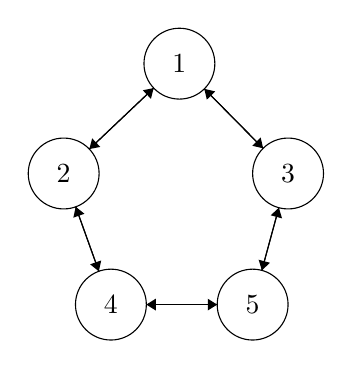
\begin{tikzpicture}[scale=0.15]
\tikzstyle{every node}+=[inner sep=0pt]
\draw [black] (41.5,-11) circle (3);
\draw (41.5,-11) node {$1$};
\draw [black] (31.7,-20.3) circle (3);
\draw (31.7,-20.3) node {$2$};
\draw [black] (50.7,-20.3) circle (3);
\draw (50.7,-20.3) node {$3$};
\draw [black] (35.7,-31.4) circle (3);
\draw (35.7,-31.4) node {$4$};
\draw [black] (47.7,-31.4) circle (3);
\draw (47.7,-31.4) node {$5$};
\draw [black] (39.32,-13.07) -- (33.88,-18.23);
\fill [black] (33.88,-18.23) -- (34.8,-18.05) -- (34.11,-17.32);
\draw [black] (33.88,-18.23) -- (39.32,-13.07);
\fill [black] (39.32,-13.07) -- (38.4,-13.25) -- (39.09,-13.98);
\draw [black] (32.72,-23.12) -- (34.68,-28.58);
\fill [black] (34.68,-28.58) -- (34.88,-27.66) -- (33.94,-27.99);
\draw [black] (34.68,-28.58) -- (32.72,-23.12);
\fill [black] (32.72,-23.12) -- (32.52,-24.04) -- (33.46,-23.71);
\draw [black] (49.92,-23.2) -- (48.48,-28.5);
\fill [black] (48.48,-28.5) -- (49.17,-27.86) -- (48.21,-27.6);
\draw [black] (44.7,-31.4) -- (38.7,-31.4);
\fill [black] (38.7,-31.4) -- (39.5,-31.9) -- (39.5,-30.9);
\draw [black] (38.7,-31.4) -- (44.7,-31.4);
\fill [black] (44.7,-31.4) -- (43.9,-30.9) -- (43.9,-31.9);
\draw [black] (48.59,-18.17) -- (43.61,-13.13);
\fill [black] (43.61,-13.13) -- (43.82,-14.05) -- (44.53,-13.35);
\draw [black] (43.61,-13.13) -- (48.59,-18.17);
\fill [black] (48.59,-18.17) -- (48.38,-17.25) -- (47.67,-17.95);
\draw [black] (48.48,-28.5) -- (49.92,-23.2);
\fill [black] (49.92,-23.2) -- (49.23,-23.84) -- (50.19,-24.1);
\end{tikzpicture}
\end{center}


Next, we show that every group of $n \geq 6$ people must have 3-mutuality. Again, write $p_{ij}$ to denote that $i$ is a friend of $j$.  

Let $G=\{1,\ldots,6\}$ and sort the five people $2,\ldots,6$ into two pigeonholes according to the truth value, true ($\top$) or false ($\bot$) of $p_{12},\ldots,p_{16}$. That is, sort people $2,\ldots,6$ into two groups, one group which are all friends of $1$, and one group all of which are not friends with $1$. By Principle \ref{MPHP}, one of these holes, suppose it's the $\top$ one, contains at least three members of $G$.

Now, either two of these are friends, in which case they, together with $1$ form a collection of three mutual friends, or none of them of friends, in which case they themselves form a collection of three mutual strangers. The argument is analogous in the case that three members of $G$ were sorted into the $\bot$ pigeonhole. 
\end{proof}

\begin{aside}
We might wonder whether every natural number $n$ has a $k$ such that every group of at least size $k$ has $n$-mutuality. This happens to be true (try proving it!). The \emph{Ramsey number} $R_{m, n}$ is the least $k$ such that every set of $k$ people must have either a group of $m$ mutual friends or $n$ mutual strangers. In the previous example, we showed that $R_{3, 3} = 6$. Higher Ramsey numbers are much harder to compute. We know that $R_{4, 4} = 18$. $R_{5, 5}$ is currently known to be between $43$ and $48$. $R_{6, 6}$ is somewhere between $102$ and $165$. 

As an exercise, prove that $R_{m, n} = R_{n, m}$ for all $m, n$.

``Suppose aliens invade the earth and threaten to obliterate it in a year's time unless human beings can find the Ramsey number for red five and blue five. We could marshal the world's best minds and fastest computers, and within a year we could probably calculate the value. If the aliens demanded the Ramsey number for red six and blue six, however, we would have no choice but to launch a preemptive attack.'' - Paul Erdos
\end{aside}

Love differs from friendship in that there are narcissists (so we can't assume the relation is irreflexive) and is not always requited (so we can't assume the relationship is symmetric). This difference between friendship and love allows the existence of numerically diverse groups of lovers, that is, groups where each person in the group loves a different number of people in the group. Consider, for example, a group of four people, $\{1, 2, 3, 4\}$. Suppose that $1$ doesn't love anyone, $2$ loves $1$, $3$ loves both $1$ and $2$, and $4$ loves all of $1,2$, and $3$, and that this exhausts all the love among our group of four. We achieve numerical diversity at the sacrifice of requital. 

\begin{center}
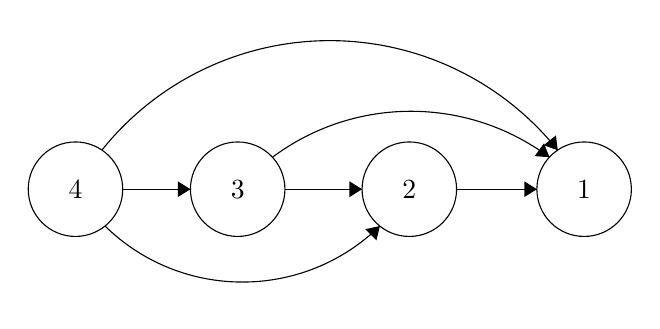
\begin{tikzpicture}[scale=0.2]
\tikzstyle{every node}+=[inner sep=0pt]
\draw [black] (53.2,-20.3) circle (3);
\draw (53.2,-20.3) node {$1$};
\draw [black] (42.1,-20.3) circle (3);
\draw (42.1,-20.3) node {$2$};
\draw [black] (31.2,-20.3) circle (3);
\draw (31.2,-20.3) node {$3$};
\draw [black] (20.9,-20.3) circle (3);
\draw (20.9,-20.3) node {$4$};
\draw [black] (45.1,-20.3) -- (50.2,-20.3);
\fill [black] (50.2,-20.3) -- (49.4,-19.8) -- (49.4,-20.8);
\draw [black] (34.2,-20.3) -- (39.1,-20.3);
\fill [black] (39.1,-20.3) -- (38.3,-19.8) -- (38.3,-20.8);
\draw [black] (33.405,-18.273) arc (126.74959:53.25041:14.7);
\fill [black] (51,-18.27) -- (50.65,-17.39) -- (50.06,-18.2);
\draw [black] (40.229,-22.635) arc (-45.59639:-134.40361:12.474);
\fill [black] (40.23,-22.64) -- (39.31,-22.84) -- (40.01,-23.55);
\draw [black] (22.578,-17.817) arc (141.31542:38.68458:18.54);
\fill [black] (51.52,-17.82) -- (51.41,-16.88) -- (50.63,-17.51);
\draw [black] (23.9,-20.3) -- (28.2,-20.3);
\fill [black] (28.2,-20.3) -- (27.4,-19.8) -- (27.4,-20.8);
\end{tikzpicture}
\end{center}

How many different patterns of love might obtain among a group of four people $\{1,2,3,4\}$? Let's recycle the sentence letters and use $p_{ij}$ to signify the statement that $i$ loves $j$; note that 16 sentence letters would be required to record all the relevant statements. Since each pattern of love among $1,2,3,4$ is determined by assigning one of the truth values $\top$ or $\bot$ to each of these 16 sentence letters, we can conclude that the number of such patterns is $2^{16}$. Why? Because there are two assignments to $p_{11}$ and for each of these, there are two assignments to $p_{12}$, and thus $2\cdot 2 = 2^2$ assignments to them jointly (this observation is given the exalted title, ``The Product Rule''). Thus, by iterating application of the product rule another fourteen times, we arrive at the conclusion that there are $2^{16}$ possible truth assignments to the 16 sentence letters. 

\begin{aside}
    $2^{16} = 65536$. It's kind of amazing that there are as many as 65,536 different potential love-scenarios at a table for four!
\end{aside}

Friendship, as compared to love, is relatively tame in terms of the number of scenarios that might arise. Let's return to using $p_{ij}$ to indicate that $i$ and $j$ are friends. In virtue of the fact that friendship is symmetric and irreflexive, a friendship-scenario is determined by assigning one of the truth values $\top$ or $\bot$ to each of the 6 sentence letters $p_{ij}$, for $1\leq i < j\leq 4$. Hence, there are only $2^6=64$ possible patterns of friendship among the group of four, less than 1/1000 of the number of potential love-scenarios. 

\begin{aside}
In general, how many possible friendship scenarios are there among a group of $n$ people? Well, every pair can either be friends or not friends, so there are $2^{num\_pairs}$ possibilities. How many pairs are their, in terms of $n$? 
\end{aside}

\newpage

\subsection{Review}
\begin{mdframed}[linewidth=1]
\section*{Concept Review}
\begin{itemize}
    \item \textbf{Pigeonhole Principle}: If you have $n + 1$ pigeons and you try to fit them all into $n$ holes, then there has to be at least one hole with $k > 1$ pigeons. 

    \item \textbf{The Mean Pigeonhole Principle}: If you distribute $m$ pigeons into $n$ pigeonholes and $m\geq k\cdot n +1$, then some hole contains at least $k+1$ pigeons. 

    \item \textbf{Product Rule}: If there are $n$ ways to do a first action and $m$ ways to do a second action, there are $n\cdot m$ ways to do both action 1 and action 2. 
\end{itemize}
\end{mdframed}


\newpage
\begin{mdframed}[linewidth=1]
\section*{Problems}
\begin{enumerate}
    \item Let $X$ be a set, $|X| = n$ (we write $|X|$ for the size of the set $X$). How many subsets does $X$ have? 

    \item How many subsets of even size does a set $X$ of size $n>0$ have?

    \item Prove that the Cartesian plane cannot be colored using only two colors (Red/Blue) such that all points 1 unit away from each other are different colors. 

    \item Prove that for any set of $n \geq 2$ numbers, there are $2$ numbers whose difference is divisible by $n - 1$. 

    \item Show that for any $n \in \mathbb{N}$, there is a number $k$ whose base ten numeral contains only ``$5$''s and ``$0$''s such that $k$ is divisible by $n$.  
\end{enumerate}
\end{mdframed}

\newpage
\begin{mdframed}[linewidth=1]
\section*{Solutions}
\begin{enumerate}
    \item There are $2^n$ many subsets of a set of size $n$. To see why this is the case, note that every element of the set can be either in or not in any given subset. Hence there are two choices for each of the $n$ elements of the set, and by the product rule $2^n$ choices in total. 

    \item $2^{n-1}$. 
    We show that for every $X$ of size at least one, the number of even-size subsets of $X$ is equal to the number of odd-size subsets of $X$; it then follows from the result of the preceding problem that the answer is $2^{n-1}$. 
    
    First, suppose that the size of $X$ is odd. Then complementation induces a one-to-one correspondence between the odd-size and even-size subsets of $X$. That is, we associate to each odd-size subset $Y\subseteq X$, the even-size subset $X-Y$. If, on the other hand, the size $n>1$ of $X$ is even, we argue as follows. Let $a$ be an element of $X$ and consider the set $W=X-\{a\}$. Since the size of $W$ is odd, we already know that it has the same number of subsets of even-size as it does of odd-size; that is, there are the same number of subsets of $X$ of odd-size that exclude $a$ as there are subsets of $X$ of even-size that exclude $a$.  From this it follows at once that also $X$ has the same number of sets of even-size that include $a$ as it does subsets of odd-size that include $a$. Thus, $X$ has the same number of subsets of odd-size as it does subsets of even-size.
    
        %Consider any nonempty subset $Y$ of $X$. Pick one element (let's call it $y$) in $Y$ and remove it from $Y$ to create a new subset $Y'$. Note that exactly one of $Y$ and $Y'$ are even: the inclusion of exlusion of $y$ corresponds to the one even and one odd subset. In this way we have associated each even subset with an odd one, and vice versa. Hence there are the same number of even and odd subsets. Since there are $2^n$ total subsets, it follows that there are $2^n/2 = 2^{n-1}$ ones of even size. 

    \item Consider an equilateral triangle with unit-length sides. We have three points pairwise one-unit apart and only two colors. The answer follows by application of the pigeonhole principle. 

    \item Note that there are $n - 1$ remainders when dividing by $n - 1$. Hence by the pigeonhole principle two of our $n$ numbers must have the same remainder when divided by $n - 1$. Their difference is divisible by $n - 1$. 

    \item Consider the first $n + 1$ elements of the set $\{5, 55, 555...\}$. We know from above that this set has two numbers whose difference is divisible by $n$. Note that the difference of any two numbers in this set is written using only $5$s and $0$s.

\end{enumerate}
\end{mdframed}
\newpage

\section{Truth-Functional Logic}

\subsection{Introduction to Truth-Functional Logic}
Throughout the course we will see a few different systems for formalizing statements. Each consists of a formal language to represent statements, and a way to interpret the meaning of statements in that language. Truth-functional logic is the simplest of these systems we will learn. 

\subsubsection*{Components of Truth Functional Logic}
\begin{enumerate}
    \item Language (the \emph{Syntax})
    \begin{enumerate}
        \item sentence letters
        \item connectives
    \end{enumerate}
    \item Interpretation (the \emph{Semantics})
    \begin{enumerate}
        \item A function that assigns $\top$ or $\bot$ (true or false) to each sentence letter, called a \textbf{truth-assignment}
        \item Fixed \textbf{truth-functional semantics} for each connective
    \end{enumerate}
\end{enumerate}

\textbf{Sentence letters} such as $p, q, r, \ldots$ schematize statements (in natural language) which are true or false, and \textbf{connectives} such as $\wedge, \vee, \neg, \supset, \ldots$ are used to combine sentence letters into compound schemata. 

\begin{aside}
Statements are sentences whose truth or falsity is independent of context of utterance. For example, the sentence ``I am bald'' is not a statement, since the truth or falsity of a given utterance of this sentence depends not only on the speaker and the time of utterance, but also on whatever subtle contextual factors might partially restrict the the range of application of the vague term ``bald.'' On the other hand, ``eight times seven is fifty-four'' is as a statement, since it's truth or falsity (in this case falsity) is independent of context of utterance. Neither of the sentences ``is eight times seven fifty-four?'' nor ``please, let eight times seven be fifty-four,'' is a statement. Truth-functional logic deals with the truth or falsity of \emph{statements} only, and we use sentence letters exclusively to schematize statements. 
\end{aside}

\newpage
\subsection{Basic Syntax of Truth-Functional Logic}
Consider using the sentence letter $p_{ij}$ to schematize the statement ``$i$ loves $j$,'' where $1\leq i,j,\leq 4$. For example, $p_{11}$ schematizes the statement ``1 loves 1'', or briefly, ``1 is a narcissist.'' 

Suppose we wish to schematize the following statements using those sentence letters: 

\begin{enumerate}
\item all of 1, 2, 3, and 4 are narcissists;\label{allnar}
\item none of 1, 2, 3, and 4 are narcissists;\label{nonar}
\item at least one of 1, 2, 3, and 4 is a narcissist;\label{onenar}
\item an odd number of 1, 2, 3, and 4 are narcissists.\label{oddnar}
\end{enumerate} 

In order to do so, we introduce the following truth-functional connectives. For each connective, we display its truth-functional interpretation via a table indicating the truth value of the compound schema as a function of the truth values of its components.
\begin{itemize}
\item Conjunction (and):
\[
\begin{array}{|l|l|c|} \hline
p   & q  &  (p \wedge q)   \\ \hline
\top & \top & \top  \\
\top & \bot & \bot  \\
\bot & \top & \bot  \\
\bot & \bot & \bot \\
\hline
\end{array}
\]
\item Negation (not):
\[
\begin{array}{|l|c|} \hline
p   &  \neg p    \\ \hline
\top & \bot  \\
\bot & \top  \\
\hline
\end{array}
\]
\item Inclusive Disjunction (or)
\[
\begin{array}{|l|l|c|} \hline
p   & q  &  (p \vee q)   \\ \hline
\top & \top & \top  \\
\top & \bot & \top  \\
\bot & \top & \top  \\   
\bot & \bot & \bot \\
\hline
\end{array}
\]

\item Exclusive Disjunction (exclusive or, xor)
\[
\begin{array}{|l|l|c|} \hline
p   & q  &  (p \oplus q)   \\ \hline
\top & \top & \bot  \\
\top & \bot & \top  \\
\bot & \top & \top  \\
\bot & \bot & \bot  \\
\hline
\end{array}
\]

\item Material Conditional
\[
\begin{array}{|l|l|c|} \hline
p   & q  &  (p \supset q)   \\ \hline
\top & \top & \top  \\
\top & \bot & \bot  \\
\bot & \top & \top  \\   
\bot & \bot & \top \\
\hline
\end{array}
\]

\item Material Biconditional
\[
\begin{array}{|l|l|c|} \hline
p   & q  &  (p \equiv q)   \\ \hline
\top & \top & \top  \\
\top & \bot & \bot  \\
\bot & \top & \bot  \\   
\bot & \bot & \top \\
\hline
\end{array}
\]
\end{itemize}


The definitions of the truth-functional connectives suffice to determine the truth/falsity of a compound schema completely in terms of (eg as a function of) the truth/falsity of its components. Hence, the term ``truth-functional logic.'' 


We can now schematize conditions \ref{allnar} -- \ref{oddnar} in the above example as follows.

\begin{enumerate}
\item[S1:] $((p_{11}\wedge p_{22})\wedge p_{33})\wedge p_{44}$\label{sallnar}
\item[S2:] $((\neg p_{11}\wedge\neg p_{22})\wedge\neg p_{33})\wedge\neg p_{44}$\label{snonar}
\item[S3:] $((p_{11}\vee p_{22})\vee p_{33})\vee p_{44}$\label{sonenar}
\item[S4:] $((p_{11}\oplus p_{22})\oplus p_{33})\oplus p_{44}$\label{sevennar}
\end{enumerate}

The first three are quite straightforward to verify; the fourth we will prove later in Proposition \ref{parity-prop}. 


\newpage
\subsection{Basic Semantics of Truth-Functional Logic}
Given a truth-functional schema like $((p \wedge q) \vee r)$, we cannot determine whether the schema is true or false unless we know whether $p$, $q$, and $r$ are true or false. That is, any schema requires a truth-assignment to its sentence letters before it can be evaluated. 

\begin{definition}[Truth-assignment]
Let $X$ be a set of sentence letters. A \emph{truth-assignment} $A$ for $X$ is a mapping which associates with each sentence letter $q\in X$ one of the two truth values $\top$ or $\bot$; we write $A(q)$ for the value that $A$ associates to $q$. 
\end{definition}

\begin{definition}
Suppose $S$ is a truth-functional schema such that every sentence letter with an occurrence in $S$ is a member of $X$. We say a truth assignment $A$ for $X$ \emph{satisfies} such a schema $S$ (and write $A\models S$) if and only if $S$ receives the value $\top$ relative to the truth assignment $A$. 
\end{definition}

\begin{example}
Take the schema $S = ((p \wedge q) \vee r)$, with truth assignment $A$ such that $A(p) = \top$, $A(q) = \bot$, and $A(r) = \bot$, we have that $S$ receives the value $\bot$. In other words $A$ does not satisfy $S$. ($A \not \models S$).
\end{example}

\subsubsection*{Interpreting the Material Conditional}
Let's return to our potential lovers and restrict attention to just two of them, 1 and 2. How could express the statement that all love is requited among these two sweethearts? The natural mode of expression is: if 1 loves 2, then 2 loves 1, and if 2 loves 1, then 1 loves 2. This is a perfect candidate for using the material conditional.

Using the sentence letters $p_{11}, p_{12}, p_{21}, p_{22}$ as earlier interpreted, we can express the happy state that all love among 1 and 2 is requited by the schema
\[ 
    R: (p_{12}\supset p_{21}) \wedge (p_{21}\supset p_{12})
\]
or, equivalently, 
\[
    p_{12} \equiv p_{21}
\]

\begin{aside}
    In how many of the possible love scenarios among 1 and 2 is all love requited? Count the number of satisfying truth-assignments to $R$!
\end{aside}

While the motivations for the truth-functional definitions for the other connectives normally seem evident to new logicians, the material conditional often gives people trouble. Let's consider generalized conditionals as a route to motivating the truth-functional interpretation of the conditional offered above. Of course, the statement ``if an integer is divisible by six, then it is divisible by three,'' is true, and thence each of the following statements, which are instances of this
general statement, are true.
\begin{itemize}
\item ``If twelve is divisible by six, then twelve is divisible by three.''
\item ``If three is divisible by six, then three is divisible by three.''
\item ``If two is divisible by six, then two is divisible by three.''
\end{itemize}
%Note that the preceding sentences are in the form $\top \supset \top$, $\bot \supset \top$, and $\bot \supset \bot$ respectively. 

Therefore, if the conditional involved is to be understood truth-functionally, then its interpretation must satisfy the conditions imposed by the first, third, and fourth rows of the material conditional's truth-table. On the other hand, the falsity of the conditional ``if twelve is divisible by six, then twelve is divisible by seven,'' mandates the condition imposed by the second row of the truth-table.

\subsubsection*{An Inductive Proof}
Let's do a simple inductive proof about truth-functional satisfaction, as an illustration of the use of mathematical induction, especially in application to reasoning about truth-functional schemata.

\begin{proposition}\label{parity-prop}
For every $n\geq 2$ and every set $X=\{q_1,\ldots,q_n\}$ of $n$ distinct sentence letters, a truth assignment $A$ for $X$ satisfies the schema
\[S_n: (\ldots(q_1\oplus q_2)\ldots\oplus q_n)\]
if and only if $A$ assigns an odd number of the sentence letters in $X$ the value $\top$.
\end{proposition}

\begin{proof}
    We prove the proposition by induction on $n$. 
    \begin{itemize}
        \item Basis: Examination of the truth table for $\oplus$ suffices to establish the proposition for the case $n=2$.

        \item Induction Step: Suppose the proposition holds for a number $k\geq 2$, that is, 
        for every truth assignment $A$ for $\{q_1,\ldots,q_k\}$, $A\models S_k$ if and only if $A$ assigns an odd number of the sentence letters in $\{q_1,\ldots,q_k\}$ the value $\top$; this is our induction hypothesis.
        We proceed to show that the proposition also holds for $k+1$. Let $A'$ be an assignment to the sentence letters 
        $\{q_1,\ldots,q_{k+1}\}$ and let $A$ be its restriction to $\{q_1,\ldots,q_k\}$. We consider two cases. First, suppose that $A'(q_{k+1}) = \top$. In this case, $A'\models S_{k+1}$ if and only if $A\not\models S_k$ if and only if (by our induction hypothesis) $A$ assigns an even number of the sentence letters $\{q_1,\ldots,q_k\}$ the value $\top$. Hence, if $A'(q_{k+1}) = \top$, then $A'\models S_{k+1}$ if and only if $A'$ assigns an odd number of the sentence letters in $\{q_1,\ldots,q_{k+1}\}$ the value $\top$. On the other hand, suppose that $A'(q_{k+1}) = \bot$. In this case, $A'\models S_{k+1}$ if and only if $A\models S_k$ if and only if (by our induction hypothesis) $A$ assigns an odd number of the sentence letters $\{q_1,\ldots,q_k\}$ the value $\top$. Hence, if $A'(q_{k+1}) = \bot$, then $A'\models S_{k+1}$ if and only if $A'$ assigns an odd number of the sentence letters in $\{q_1,\ldots,q_{k+1}\}$ the value $\top$. This concludes the proof, since either $A'(q_{k+1}) = \top$ or $A'(q_{k+1}) = \bot$. 
    \end{itemize}
\end{proof}

\subsubsection*{The Centrality of Satisfaction}

The satisfaction relation is the fundamental semantic relation. It is where language and the world meet; in the case to hand, language consists of truth-functional schemata and the possible worlds they describe are truth assignments to sentence letters. As the course progresses, we will encounter more textured representations of the world (relational structures) and richer languages to describe them (monadic and polyadic quantification theory). We now define some of the central notions of truth-functional logic in terms of satisfaction. These definitions will generalize directly to the more textured structures and richer languages we encounter later. 

For the following definitions, we suppose that $S$ and $T$ are truth-functional schemata and that $A$ ranges over truth assignments to sets of sentence letters which include all those that occur in either $S$ or $T$.

\begin{definition}\label{tf-eq-sat-val-def}
$S$ \emph{implies} $T$ if and only if for every truth assignment $A$, if $A\models S$, then $A\models T$.
\end{definition}

\begin{definition}
$S$ is \emph{equivalent} to $T$ if and only if $S$ implies $T$ and $T$ implies $S$
\end{definition}

\begin{definition}
$S$ is \emph{satisfiable} if and only if for some $A$, $A\models S$.
\end{definition}

\begin{definition}
$S$ is \emph{valid} if and only if every truth assignment satisfies $S$. 
\end{definition}
\subsubsection*{Examples of equivalence and the material biconditional}

Try to see why the following are equivalent - either by appealing to your understanding of what the connective ``means'' or by going back to the truth tables. 

\begin{itemize}
\item $p\oplus q$ is equivalent to $q\oplus p$ (commutativity of exclusive disjunction)  
\item $(p\oplus q)\oplus r$ is equivalent to $p\oplus(q\oplus r)$ (associativity of exclusive disjunction).
\item $p \equiv q$ ius equivalent to $(p \supset q) \land (q \supset p)$
\end{itemize}

Note that both conjunction and inclusive disjunction are also commutative and associative, whereas the material conditional is neither. 

\begin{aside}
    Try to to think of examples of (binary) truth-functional connectives which are commutative but not associative, and associative but not commutative.
\end{aside}

\newpage
\subsection{Review}
\begin{mdframed}[linewidth=1]
\section*{Concept Review}
\textbf{Definitions}
\begin{itemize}
    \item A truth-assignment $A$ for $X$ is a function which maps every sentence letter $q \in X$ to either $\top$ or $\bot$. $A(q)$ is the notation for the value $A$ associates with $q$.

    \item A schema $S$ \emph{implies} a schema $T$ iff for all truth-assignments $A$, if $A \models S$ then $A \models T$.
    
    \item A schema $S$ is \emph{equivalent} to a schema $T$ iff $S$ and $T$ are satisfied by exactly the same truth assignments (for all $A$, $A \models S$ iff $A \models T$). 
    
    \item $S$ is \emph{satisfiable} iff there is a truth assignment that satisfies it (there exists an $A$ such that $A \models S$)
    
    \item $S$ is \emph{valid} iff all truth assignments satisfy it (for all $A$, $A \models S$)
\end{itemize}

\textbf{Syntax, Semantics}
The \emph{syntax} of TF-logic is given by the rules for forming truth-functional schemata from sentence letters and connectives. The \emph{semantics} of TF-logic are given by a \emph{truth-assignment}, which associates with each letter a \emph{truth-value}.

\textbf{Satisfying Sentences}
The \emph{truth-values} of the individual sentence letters in a schema are propagated to the whole schema by means of \emph{truth-tables} which give fixed semantic interpretations to each of the \emph{connectives}. We say that a truth-assignment $A$ \emph{satisfies} a sentence $S$ (written $A \models S$) iff the sentence $S$ evaluates to $\top$ under the truth-assignment $A$. Otherwise, we write $A \not \models S$ and say that $A$ does not satisfy $S$. 
 
\end{mdframed}

\newpage
\begin{mdframed}[linewidth=1]
\section*{Problems}
\begin{enumerate}
    \item Is ``the University of Pennsylvania has a Logic major'' a statement? Why or why not? 

    \item Is ``should I major in Logic?'' a statement? Why or why not?

    \item Using the sentence letters $p_{ij}$, $q \leq i, j \leq 4$ to stand for ``person $i$ loves person $j$''. Schematize the following statements:
    \begin{enumerate}
        \item Person 1 loves everyone else.

        \item There is a Shakespearean love triangle (\emph{i.e.}, no one has their love requited) between people 1, 2, 3, and person 4 is a Scrooge (he does not love anyone, even himself). 

        \item Everyone loves, exclusively, people with numbers lower than themselves. 
    \end{enumerate}

    \item How many truth-assignments to the given letters satisfy the following schema?
    \[
        (p_1 \supset q_1) \land ... \land (p_5 \supset q_5)
    \]

    \item How many truth-assignments to the set of sentence letters $X_n=
    \{p_1,q_1,\ldots,p_n,q_n\}$ satisfy the following schema $S_n$? Express your answer as a function of $n$ and prove that it is correct by mathematical induction. 
    \[
      (p_1 \supset q_1) \land ... \land (p_n \supset q_n)  
    \]

    \item How many truth-assignments over the given letters satisfy the following schema?
    \[
        p_1 \oplus p_2 \oplus p_3 \oplus p_4 \oplus p_5
    \]

     \item Is the following sentence valid, satisfiable but not valid, or unsatisfiable?
    \[
        (a \equiv b) \supset (a \vee \lnot b)
    \]

    \item Valid, satisfiable, or unsatisfiable?
    \[
        (b \vee (b \supset a)) \land (\lnot b \vee (a \supset b))
    \]

    \item Valid, satisfiable, or unsatisfiable?
    \[
        (a \equiv b) \land (b \equiv c) \land (a \oplus b)
    \]

    \item How many truth-assignments for the given letters satisfy 
    \[
         (a \equiv b) \land (b \equiv c) \land (c \equiv d)
     \] 

     \item How many truth-assignments to the given letters satisfy
    \[
        (a \oplus b) \vee (b \oplus c) \vee (c \oplus d)
    \]

    \item I claim that if $n$ people all shake hands with each other (once per pair), the total number of handshakes is $\frac{n(n-1)}{2}$. Prove this by induction. 
\end{enumerate}
\end{mdframed}
\newpage
\begin{mdframed}[linewidth=1]
\section*{Solutions}
\begin{enumerate}
    \item Yes, it is.\footnote{Although, one might insist that there remains an element of context dependence owing to an ambiguity in the proper name ``University of Pennsylvania'' - those in Indiana County, Pennsylvania might well use it to refer to a different institution. This observation invites reflection upon the intriguing question whether (virtually) all sentences of ordinary language are to some extent context dependent (at least without non-ordinary supplementation).}  

    \item No, it is not. It is not a statement because it expresses a question, which is not determinitely true or false. 

    With that being said, you should - of course - major in logic\footnote{Provided you like it and want to.}.

    \item 
    \begin{enumerate}
        \item $p_{11} \land p_{12} \land p_{13} \land p_{14}$

        \item $((p_{12} \land p_{23} \land p_{31}) \vee (p_{13} \land p_{21} \land p_{32})) \land \lnot(p_{41} \vee p_{42} \vee p_{43} \vee p_{44})$

        \item $p_{21} \land p_{31} \land p_{32} \land p_{41} \land p_{42} \land p_{43}$
    \end{enumerate}

    \item $3^5$. Note that each of the terms of the form $p_i \supset q_i$ is satisfied in three cases (check the truth table) and apply the product rule. 

    \item $3^n$ for $n \geq 1$. 

    BASE CASE: Verify, via the truth table for the material conditional, that three of the four truth assignments to $X_1=\{p_1,q_1\}$ satisfy the schema $S_1$. 

    INDUCTION STEP: Suppose that $3^n$ of the  $4^n$ truth-assignments to $X_n$ satisfy $S_n$:
    \[ 
    (p_1 \supset q_1) \land ... \land (p_n \supset q_n). 
    \]
    Let $A$ be one such truth-assignment. Verify, using the truth-table for the material conditional, that $A$ may be extended to exactly  three distinct truth-assignments to the sentence letters $X_{n+1}$ each of which satisfies $S_{n+1}$. It follows that   there are $3\cdot3^n=3^{n + 1}$ truth-assignments to the sentences letters $X_{n+1}$ that satisfy $S_{n + 1}$: 
    \[ 
    (p_1 \supset q_1) \land ... \land (p_n \supset q_n) 
    \land (p_{n + 1} \supset q_{n + 1}). 
    \] 
    %Note that there are $3$ satisfying assignments to $S$ and $s_{n + 1}$ which satisfy $S \oplus s_{n + 1}$. By hypothesis there are $3^n$ truth assignments satisfying $(p_1 \supset q_1) \land ... \land (p_n \supset q_n) = S_n$. By the product rule then, there are $3^n \cdot 3 = 3^{n + 1}$ total satisfying assignments to $S_n \land s_{n + 1}$ as required. 

    \item $2^4 = 16$. Remember that there are $2^{n-1}$ ways to pick an odd-sized subset from $n$ elements and that a sentence of the given form is satisfied iff an odd number of sentence letters are set to true. 

    \item This is valid. Suppose $A$ is a truth-assignment to the sentence letters $a$ and $b$. Note that if $A(a \equiv b)=\bot$, then $A$ satisfies the given schema. So suppose $A(a \equiv b)=\top$. Then $A(a)=A(b)$, hence either $A(a)=\top$ or $A(b)=\bot$. Thus $A(a \vee \lnot b)=\top$. %holds (since one of $a$ or $\lnot b$ must be true, hence the consequent is true, hence the conditional is true). If $a$ is not equivalent to $b$, then the conditional holds because false implies anything. 

    \item Valid. Suppose $A$ is a truth-assignment to the sentence letters $a$ and $b$. If $A(b)=\top$, then $A$ clearly satisfies the left conjunct. If $A(b)=\bot$, then $A(b \supset a)=\top$, hence $A$ satisfies the left conjunct  as well. Similarly, if $A(b)=\top$, then $A$ satisfies the right conjunct, and if $A(b)=\bot$, then $A(\lnot b)=\top$, hence again $A$ satisfies the right conjunct. 

    \item Unsatisfiable. Suppose $A$ is a truth-assignment to the sentence letters $a,b$ and $c$ and $A$ satisfies both $a\equiv b$  and $b\equiv c$. It follows that $A$ satisfies $a\equiv c$ (in other words, $\equiv$ is \emph{transitive}). But then $A$ does not satisfy $a \oplus c$, since this is truth-functionally equivalent to $\lnot (a\equiv c)$. So the schema is unsatisfiable. 

    \item 2. Picking true/false for $a$ fixes the truth-values of the remaining letters. 

    \item 14. To get this answer, we note that there are 16 ($2^4$) truth-assignments in total; count the number which do not satisfy our sentence, and subtract that number from 16. The sentence is only not satisfied when each of $a, b, c, d$ have the same truth-value, so there are 2 non-satisfying truth-assignments. This means there are $16 - 2 = 14$ satisfying truth assignments. 

    \item BASE CASE: $n = 2$. Two people shaking hands results in one handshake, and the formula gives us $\frac{2(2-1)}{2} = 1$ which is correct. Note that we pick $n = 2$ as the base case (not $n = 0$ or $n = 1$) because it doesn't really make sense to talk about those cases (since you need two people for a handshake). 

    INDUCTIVE CASE: Assume that for $n$ people, the number of handshakes (let's denote it $H_n$) is $H_n = \frac{n(n-1)}{2}$. We want to show (henceforth ``wts'') that for $n + 1$ people the number of handshakes is $H_{n+1} = \frac{(n+1)n}{2}$. The number of handshakes between $n + 1$ people is clearly the number of handshakes for $n$ people ($H_n$) plus $n$, since our new person must shake hands with the $n$ others. So we have $H_{n+1} = H_n + n = \frac{n(n-1)}{2} + n = \frac{n^2 - n + 2n}{2} = \frac{n^2 + n}{2} = \frac{(n+1)n}{2}$, which is what we wanted to show. 

\end{enumerate}
\end{mdframed}

\newpage
\subsection{Expressive Completeness of Truth Functional Logic}
\begin{definition}
    We use the symbol $:=$ to mean ``is defined to be equal to''. $:=$ expresses a \emph{definition} of equality, whereas $=$ expresses a statement about equality.

    If you're a coder, $x := 10$ is to logic/math as \verb|let x = 10| is to JavaScript, whereas $x = 10$ is to logic as \verb|x === 10| is to JavaScript.
\end{definition}

\subsubsection*{Propositions as a heuristic}
It is sometimes useful to think of a schema $S$ as expressing a proposition, to whit, the set of truth assignments $A$ that satisfy $S$; of course, this needs to be relativized to a collection of sentence letters $X$ which includes all those occurring in $S$. We suggested the notation: 
\[\prop{S}{X} = \{ A\mid A\  \mbox{is a truth assignment for $X$ and } A\models S\}.
\]
 When we use this notation without the subscript $X$, we assume $A$ is a truth assignment for exactly the set of sentence letters with occurrences in $S$. 

\subsubsection*{Expressive Completeness}
In the last section, we used the notion of the proposition expressed by a schema as an intuitive vehicle for pursuing this investigation. Since the semantical correlate of a truth-functional schema is a set of truth assignments to some finite set of sentence letters, we can frame the question of the \emph{expressive completeness of truth-functional logic} in terms of propositions. Let $X$ be a non-empty finite set of sentence letters. We deploy the notation: $\mathbb{A}(X)$ for the set of truth assignments to the sentence letters $X$, and $\mathbb{S}(X)$ for the set of truth-functional schemata compounded from sentence letters all of which are members of $X$. 

We provide the following inductive definition of $\mathbb{S}(X)$. 
\begin{definition}
Let $X$ be a nonempty finite set of sentence letters. $\mathbb{S}(X)$ is the smallest set $\mathbb{U}$ (in the sense of the subset relation) satisfying the following conditions.
\begin{itemize}
\item $X\subseteq \mathbb{U}$.
\item If $\sigma$ and $\tau$ are strings over the finite alphabet $X\cup\{),(,\neg,\supset,\equiv,\vee,\wedge,\oplus\}$, and $\sigma,\tau\in\mathbb{U}$, then each of the strings $\neg\sigma, (\sigma\supset\tau),(\sigma\equiv\tau),(\sigma\vee\tau),(\sigma\wedge\tau),(\sigma\oplus\tau)$ belong to $\mathbb{U}$.\footnote{Here ``$(\sigma\supset\tau)$'' denotes the string with the initial symbol ``$($'' concatenated with the string denoted by $\sigma$ concatenated with the symbol ``$\supset$'' concatenated with the string denoted by $\tau$ and with terminal symbol ``$)$'', and likewise in all the other cases.}
\end{itemize}
\end{definition}

\begin{aside}
    This is simply a formal way of saying that all of our sentences have to use only the letters from $X$ and must be ``well-built'' in the sense that each connective has the correct number of arguments, with all the bracketing done correctly. For example, with $X := \{p, q, r\}$ then $S_1 := ((p \vee q) \land r)$ is well-built, whereas $S_2 := \vee p \land q$ is not. 
\end{aside}



If $\mfp\subseteq\mathbb{A}(X)$, we call $\mfp$ a \emph{proposition over} $X$. 

Let $X$ be a non-empty finite set of sentence letters and let $\mfp$ be a proposition over $X$. Is there a schema $S\in\mathbb{S}(X)$ such that $\prop{S}{X}=\mfp$, ie can every proposition be expressed by some schema? In other words, is truth-functional logic \emph{expressively complete}? 

\begin{theorem}[Expressive Completeness of Truth-functional Logic]\label{tflexpcomp-thm}
Let $X$ be a non-empty finite set of sentence letters and let $\mfp$ be a proposition over $X$. There is a schema $S\in\mathbb{S}(X)$ such that $\prop{S}{X}=\mfp$.
\end{theorem}

\begin{aside}
    This looks complicated, but it really isn't. In natural language, what it's saying is this: \emph{pick any subset $\mfp$} (your proposition) \emph{of truth assignments for a set of sentence letters $X$. Then there is a truth-functional schema $S$ using only letters from $X$} ($S\in\mathbb{S}(X)$) \emph{which is true only of those truth-assignments which are in $\mfp$} ($\prop{S}{X}=\mfp$). In other words, \emph{every proposion can be ``picked out'' by some schema}. This is why it's called \emph{expressive completeness}: truth-functional logic is ``expressively complete'' in that it can express every such proposition. 
\end{aside}

For the proof of Theorem \ref{tflexpcomp-thm}, the following terminology and lemma will be useful. 
\begin{definition}
Let $X$ be a non-empty finite set of sentence letters and let $S\in\mathbb{S}_X$.
\begin{itemize}
\item $S$ is a \emph{literal} over $X$ just in case $S = p$ or $S = \neg p$, for some $p\in X$.
\item $S$ is a \emph{term} over $X$ just in case $S$ is a conjunction of literals over $X$ (we allow conjunctions of length 1).
\item $S$ is in disjunctive normal form over $X$ if and only if $S$ is a disjunction of terms over $X$ (we allow disjunctions of length 1). 
\end{itemize}
\end{definition}
If $\Lambda$ is a set of literals over $X$ we write $\bigwedge \Lambda$ to abbreviate a term which is formed as a conjunction of the literals in $\Lambda$. Similarly, if $\Gamma$ is a set of terms over $X$ we write $\bigvee\Gamma$ to abbreviate a schema in disjunctive normal form which is formed as a disjunction of the terms in $\Gamma$.

\begin{example}
    Let $S = \{a, b, c\}$. Then $\bigwedge S = a \land b \land c$, and $\bigvee S = a \vee b \vee c$.
\end{example}

\begin{lemma}\label{tflexpcomp-lem}
Let $X$ be a non-empty finite set of sentence letters. For every $A\in\mathbb{A}(X)$ there is a schema $T_A$ which is a term over $X$ such that for every $A'\in\mathbb{A}(X)$
\[A'\models T_A\ \ \ \mbox{if and only if}\ \ \ A'=A.\]
\end{lemma}
\begin{proof}
Let $X$ be a finite set of sentence letters and suppose $A\in\mathbb{A}(X)$. For each $p\in X$, let $l_p = p$, if $A\models p$, and let $l_p = \neg p$, if $A\not\models p$. Let $\Lambda=\{l_p\mid p\in X\}$ and let $T_A = \bigwedge\Lambda$. It is easy to verify that
for every $A'\in\mathbb{A}(X)$, 
$A'\models T_A\ \ \ \mbox{if and only if}\ \ \ A'=A$. 
\end{proof}    

\begin{aside}
    Once you become a bit more familiar with the terminology, things will become much easier. Indeed, this lemma is really simple - in plain English, it says that \emph{for every truth assignment, there is a schema which only uses logical ANDs that is satisfied by only that truth assignment}. When stated like that, of course, it seems obvious - if your truth assignment assigns true to $p$ you should have $p$ in your schema, and if your truth-assignment assigns false to $p$, your schema should include $\lnot p$, with all the literals joined up together by ANDs. 

    The proof expresses that intuition symbolically - make sure you can understand the proof now, going over the relevant terminology and symbols if necessary. If you get stuck trying to interpret all that logical symbolism, please come into Office Hours and we'll be happy to help! Logic won't be any fun if the symbolism gets in the way of your ingenuity of understanding, so it's best if you take the time to get comfortable with all that at the start. 
\end{aside}

\begin{proof}[Proof of Theorem \ref{tflexpcomp-thm}]
Fix a finite non-empty set of sentence letters $X$ and suppose $\mfp$ is a proposition over $X$. If $\mfp=\emptyset$, then pick $p\in X$ and note that $\prop{p\wedge\neg p}{X} = \mfp$. Otherwise, for each $A\in\mfp$, choose a term $T_A$, as guaranteed to exist by Lemma \ref{tflexpcomp-lem}, such that for every $A'\in\mathbb{A}(X)$, 
$A'\models T_A\ \ \ \mbox{if and only if}\ \ \ A'=A$. Let $\Gamma = \{T_A\mid A\in\mfp\}$ and let $S=\bigvee\Gamma$. It is easy to verify that $\prop{S}{X}=\mfp$.
\end{proof}

\begin{aside}
    Once again, the main difficulty here is the symbolism - the proof expresses a simple intuition in symbolic form. Try rewriting this proof in your own words!
\end{aside}

\begin{corollary}\label{dnf-cor}
Every truth-functional schema is equivalent to a schema in disjunctive normal form.
\end{corollary}

\begin{aside}
    Corolloraries are Theorems which follow very simply or quickly from another (often proved-right-above) theorem. Whenever you see a corollary in a math textbook or notes, you should always make sure you understand why it's a consequence of the just-proven theorem!
\end{aside}

\newpage
\subsection{The Power of a Truth-Functional Schema}
We will introduce the following useful terminology.
\begin{definition} 
For the following, all schemata are drawn from $\mathbb{S}(X)$ for a fixed non-empty finite set of sentence letters $X$.
\begin{itemize}
\item 
A list of truth-functional schemata is \textit{succinct} if and only if no two schemata on the list are equivalent. 
\item 
A truth-functional schema \textit{implies a list of schemata} if and only if it implies every schema on the list.
\item The \textit{power} of a truth-functional schema is the length of a longest succinct list of schemata it implies.  
\end{itemize}
\end{definition}

\begin{example}
    Let's consider $X=\{p,q,r\}$. What is the length of a longest succinct list of truth-functional schemata over $X$? We will arrive at the answer by proving an \emph{upper bound} and a \emph{lower bound} on this length.

    \begin{itemize}
        \item Upper bound: It is easy to verify that schemata $S$ and $S'$ are equivalent if and only if $\prop{S}{}=\prop{S'}{}$. Hence, the length of a succinct list of schemata cannot exceed the number of propositions over $X$, that is, the number of subsets of the set $\mathbb{A}(X)$. The size of $X$ is 3, so the size of $\mathbb{A}(X)$ is $2^3$, since determining a truth assignment to $X$ involves three binary choices (each letter can be assigned true or false, and you make that choice for each of the three letters). By the same reasoning, the number of propositions over $X$ is $2^{2^3}$, since determining a proposition involves deciding, for each of the $2^3$ truth assignments, whether to include or omit it. Hence, the length of the longest succinct list is no more than $2^{2^3} = 2^8 = 256$.

        \item Lower bound: By Theorem \ref{tflexpcomp-thm}, for every proposition over $X$, there is a schema expressing it. Since schemata expressing distinct propositions are not equivalent, it follows at once that there is a succinct list of schemata of length 256.
    \end{itemize}
    So the longest such list is of length 256.
\end{example}

\begin{example}
    Let's compute the power, as defined above, of $p\wedge (q\vee r)$. Note that a schema $S$ implies a schema $S'$ if and only if $\prop{S}{}\subseteq\prop{S'}{}$. Thus, the power of $S$ is the number of sets $Z$ satisfying the condition: 

    \begin{equation}\label{z-eq}
        \prop{S}{}\subseteq Z\subseteq \mathbb{A}(X). 
    \end{equation}

    The size of $\mfp=\prop{p\wedge (q\vee r)}{}$ is 3, so the size of $\mathbb{A}(X)-\mfp=5$. It follows at once that $2^5 =32$ sets $Z$ satisfy condition (\ref{z-eq}); hence, the power of $p\wedge (q\vee r)$ is 32.
\end{example}

\begin{aside}
    Why is it that a schema $S$ implies a schema $S'$ if and only if $\prop{S}{}\subseteq\prop{S'}{}$? Go back to the definition of both $\prop{S}{}$ and schema implication if you need to. 

    Here's a simple way to think about it, once you know the definitions: if $S$ implies $S'$ then there is no truth assignment that satisfies $S$ but does not satisfy $S'$ (otherwise $S$ wouldn't imply $S'$, by the definition of schema implication). Hence everything that is true in $S$ is true in $S'$, or symbolically, $\prop{S}{}\subseteq\prop{S'}{}$. When written that way, it seems really simple!

    Often throughout your study of logic you will see things which, at the surface, look confusing like the statement we just considered. Make sure to always take the time to go back to definitions and understand things in your own words - it'll make logic \emph{much} more satisfying. 
\end{aside}

\begin{example}
    Let's list the numbers which are powers of truth-functional schemata over $X=\{p,q,r\}$.

    \begin{itemize}
        \item First note that for every $S,S'\in\mathbb{S}(X)$ the power of $S$ = the power of $S'$ if and only if $\size{\prop{S}{X}}=\size{\prop{S'}{X}}$, where we use $\size{U}$ to denote the number of members of the finite set $U$. 

        \item In particular, if $\mfp=\prop{S}{X}$, then the power of $S = 2^{(8-|\mathfrak{P}|)}$.

        \item It follows at once that for each $S\in\mathbb{S}(X)$, the power of $S = 2^i$, for some $0\leq i\leq 8$.
    \end{itemize}  
\end{example}

Generalizing our last example, suppose $Y$ is a finite set of sentence letters with $\size{Y}=n$. In this case
\begin{itemize}
\item $\size{\mathbb{A}(Y)}=2^n$, and 
\item for each $S\in\mathbb{S}(Y)$, if $\mfp=\prop{S}{Y}$, then the power of $S = 2^{(2^n-|\mathfrak{P}|)}$.
\end{itemize}

\begin{example}
    What is the length of a longest succinct list of truth-functional schemata over $X := {p, q, r}$ each of which has power 32?

    \begin{aside}
        Make sure you have all the relevant definitions in order - what does it mean for the power of a schema to be 32? What does it mean for a list of schemata to be succinct?  
    \end{aside}

    Well, from the definitions we know that a schema over $X := \{p, q, r\}$ has power 32 if and only if exactly three truth assignments satisfy it (why?). Hence the length of a longest such succinct list is exactly the number of subsets of size three contained in a set of size eight (why a set of size 8, given that we have 3 sentence letters?). In the next section, we'll take a break from logic proper to learn a bit about how we would determine how many such subsets there are. 
\end{example}

\subsubsection*{A Combinatorial Interlude}
Our leading question from the end of the last section brings us to an interlude on permutations and combinations: how many ways can we select $k$ members of a set of size $n$? There is an ambiguity here: are we counting modes of selection, which involve the order of choices, or collections of members selected, where the order of selection is irrelevant? Once we recognize the ambiguity, we can proceed to count both. We will need notation for each, so let $\oc{n}{k}$ for the number of ordered sequences of $k$ distinct elements that can be drawn from a set of size $n$  and $\binom{n}{k}$ for the number of subsets of size $k$ that are included in set of size $n$. 

Let's first evaluate $\oc{n}{k}$, the number of ordered sequences of size $k$ you can pick from a set of size $n$. Suppose we think of counting the ways $n$ students could fill a row of length $k$ in a lecture hall. Let's suppose the seats are labelled $1, 2, \ldots, k$. There are $n$ choices for the student to fill seat 1; once that seat is filled, there are $n-1$ choices for the student to fill seat 2; and so on until there are $(n-k)+1$ choices for the student to fill seat $k$. Hence, by the product rule, there are $n\cdot(n-1)\cdots((n-k)+1)$ ways of filling all $k$ seats, that is, $\oc{n}{k}=n\cdot(n-1)\cdots((n-k)+1)$. 

Now that we have counted the number of ordered sequences, we can see how to count the number of subsets. By the same reasoning, each subset of size $k$ appears as the content of $k\cdot(k-1)\cdots2\cdot1$ ordered sequences of length $k$; this number is called $k$ \emph{factorial} and is often abbreviated as $k!$. Hence, 
\[\binom{n}{k} = \frac{\oc{n}{k}}{k!}.\]  
Observe that 
\[\oc{n}{k}=\frac{n!}{(n-k)!}\]
from which it follows that 
\[\binom{n}{k} = \frac{n!}{k!\,(n-k)!}.\]
This last formulation makes transparent a symmetry in the values of $\binom{n}{k}$, namely, for every $k$ between $0$ and $n$, $\binom{n}{k}=\binom{n}{n-k}$. This accords nicely with the observation that complementation induces a one-one correspondence between the subsets of size $k$ and the subsets of size $(n-k)$ that can be selected from a set of size $n$. Note also that it determines in a non-arbitrary way that the value of $0!$ is 1.

\begin{aside}
    Consider picking a panel of three students from a class of 10. How many ways can you do this? Is it the same as the number of ways you could pick 7 of the 10 students to \emph{not} be on the panel, using the non-picked students for the panel?
\end{aside}

Let's not forget how this all began. Since the The length of the longest succinct list of schemata with power 32 is number of subsets of size three contained in a set of size eight, it follows that the length of the longest such list is $\binom{8}{3}=56$.

\subsubsection*{Counting the Length of an ``Implicational Anti-Chain''}
Let's use our newfound ability to count selections to answer a different question: Is there a sequence of seventy schemata $S_1,\ldots,S_{70}\in\mathbb{S}(X)$ such that for every $1\leq i\neq j\leq 70,$ $S_i$ does \emph{not} imply $S_j$? Such a sequence of schemata is called an \emph{implicational anti-chain} (of length 70).

As observed earlier, a schema $S\in\mathbb{S}(X)$ implies a schema $T\in\mathbb{S}(X)$ if and only if $\prop{S}{X}\subseteq\prop{T}{X}$. It follows that the answer to our question about an implicational anti-chain of length seventy will be the same as the answer to the following question about an anti-chain of length seventy with respect to the subset relation: Is there a list of seventy subsets of $\mathbb{A}(X)$, $P_1,\ldots,P_n$, such that for every $1\leq i\neq j\leq 70,$ $P_i$ is \emph{not} a subset of $P_j$? Note that if two finite sets, $P$ and $Q$, have the same number of members, and $P$ is not equal to $Q$, then $P$ is not a subset of $Q$ and $Q$ is not a subset of $P$. Therefore, if there are seventy distinct subsets of $\mathbb{A}(X)$ all of the same size, then the answer to our question is yes. Since $\mathbb{A}(X)$ has eight members, a positive answer to our question followed immediately by evaluating 
\[
\binom{8}{4}= \frac{8\cdot7\cdot6\cdot5}{4\cdot3\cdot2\cdot1}=70.
\] 

\begin{aside}
    Prove that if two finite sets, $P$ and $Q$, have the same number of members, and $P$ is not equal to $Q$, then $P$ is not a subset of $Q$ and $Q$ is not a subset of $P$.
\end{aside}

Note that our argument merely shows that there is an implicational anti-chain of length 70; it does not establish that there is no longer implicational anti-chain consisting of schemata in $\mathbb{S}(X)$. This is, indeed, true, but a more sophisticated argument is required to establish this result, which follows from the famous Sperner's Theorem. For a reference on Sperner's Theorem, see\footnote{Van Lint and Wilson, \emph{A course in combinatorics}, Chapter 6: Dilworth's theorem and extremal set theory.}. 


\newpage
\subsection{Is There An Efficient Decision Procedure For Truth-Functional Logic?}

It is easy to see that the finitary character of the semantics for truth-functional logic immediately yields an algorithm to decide the satisfiability of schemata of truth-functional logic. In particular, suppose $S\in\mathbb{S}(X)$ for some finite set of sentence letters $X$. Note first that for each truth-assignment $A\in\mathbb{A}(X)$ there is a simple and efficient algorithm, call it $M$, to determine whether $A \models S$. Thus, in order to test the satisfiability of $S$, we need only list $\mathbb{A}(X)$ in some canonical order $A_1,\ldots, A_{2^{|X|}}$ and use $M$ to test whether the successive $A_i$ satisfy $S$. 

\begin{aside}
    Come up with an algorithm for checking whether $A \models S$ for $A\in\mathbb{A}(X)$ and analyze its runtime complexity as a function of the length (in terms of the number of connectives) of $S$. 
\end{aside}

Of course, this algorithm is not efficient, in the sense that it's running time is potentially exponential in the length of its input. The question whether there is an efficient algorithm to decide the satisfiability of truth-functional schemata, called the $P = NP$ problem, is generally regarded as one of the most significant open mathematical problems of our time, and carries with it a \$1,000,000 prize for its solution as well as eternal mathematical glory. For further information visit: 

\verb|http://www.claymath.org/millennium-problems/p-vs-np-problem|.

\newpage
\subsection{Review}
\begin{mdframed}[linewidth=1]
\section*{Concept Review}
\textbf{Definitions}
\begin{itemize}
    \item A schema $S$ \emph{implies} a schema $T$ iff for all truth-assignments $A$, if $A \models S$ then $A \models T$. In other words, $S$ implies $T$ iff the proposition expressed by $S$ is a subset of the proposition expressed by $T$. 
    
    \item A schema $S$ is \emph{equivalent} to a schema $T$ iff $S$ and $T$ are satisfied by exactly the same truth assignments (for all $A$, $A \models S$ iff $A \models T$). In other words, $S$ and $T$ are equivalent if they express the same proposition. 

    \item $\mathbb{P}_X(S) = \{A | A \text{ is a truth assignment over } X \text{ and } A \models S\}$ is \emph{the proposition expressed by S}. It's the set of truth assignments that satisfy $S$ (where truth assignments are restricted to those for sentence letters in the set $X$). 
    
    \item $\mathbb{A}(X)$ is the set of all truth assignments over $X$. 
    
    \item A list of TF-schemata is called \emph{succinct} iff no two schema on the list are equivalent. 
    
    \item The \emph{power} of a schema $S$ is the length of the longest succint list of schemata which $S$ implies. In other words, it's the number of nonequivalent schema which $S$ implies. 
\end{itemize}

\textbf{Fun With Counting}
There are $n!$ ways to order a list of $n$ items. To see why, note that there are $n$ choices for the first element, $n - 1$ for the second, $n - 2$ for the third, resulting in $n(n - 1)(n - 2)...(1) = n!$ orderings. 

There are $\oc{n}{k} := \frac{n!}{(n-k)!}$ ways to pick an ordered list of $k$ elements from $n$ elements, $k \leq n$. As before, there are $n$ choices for the first thing, $n-1$ for the second, all the way down to $n-k+1$ for the $k^{th}$. This gives us the answer $\prod_{i = n - k + 1}^ni = \prod_{i = 1}^ni / \prod_{i = 1}^{n - k}i = \frac{n!}{(n-k)!}$   

There are $\binom{n}{k} := \frac{n!}{(n-k)!k!}$ ways to pick a subset of $k$ elements from $n$ elements, $k \leq n$. There are $\oc{n}{k}$ ordered lists of size $k$ from $n$. Since each subset of size $k$ corresponds to $k!$ orderings of those lists, we divide out by $k!$ to get $\frac{n!}{(n-k)!k!}$, which we denoted as $\binom{n}{k}$, read ``$n$ choose $k$''. 

\textbf{Expressive Completeness}

For any (arbitrary) proposition, there is a truth-functional schema which expresses that proposition. We noted that a schema can pick out individual truth-assignments by conjoining literals for each of the sentence letters (for example, the truth assignment $A_1$ which maps $p = \top, q = \top, r = \top$ is picked out by the sentence $(p \land q \land r)$). Sentences of this form are called \emph{terms}. We further noted that a disjunction of such terms (one for each truth-assignment in our proposition) was sufficient to express any proposition. 

\textbf{Power}

Suppose we have a sentence $S$ over $n$ sentence letters which is satisfied by $k$ truth assignments. Then power of $S$ is $2^{2^n - k}$. To see why this is the case, note that there are $2^n$ truth assignments for $n$ sentence letters. If $S$ is satisfied by $k$ truth assignments, then those truth assignments must also satify $T$ if $S$ implies $T$. So we can't ``choose'' to include those $k$ truth-assignments in our proposition expressed by $T$ any more, because $\mathbb{P}_X(T)$ must include them. So we are left with $2^n - k$ truth-assignments which can be in $T$ or not. Since each of these $2^n - k$ truth assignments can be either in or out of the proposition expressed by $T$, the power of $S$ is then $2^{2^n - k}$.
\end{mdframed}

\newpage
\begin{mdframed}[linewidth=1]
\section*{Problems}
For the following problems, unless otherwise specified, let $X = \{p_1 p_, p_3, p_4\}$ be the set of sentence letters under consideration. 
\begin{enumerate}
    \item What is the power of $p_1 \equiv p_2$?

    \item For four sentence letters as above, what is the length of the longest succinct list of schemata no two of which have the same power?

    \item What is the length of the longest succint list of schemata (from four sentence letters) each having power 256?

    \item What is the largest $n$ such that the conjunction of any two schema of power $n$ (with 4 sentence letters) is satisfiable?

    \item How many ways can you choose 3 marbles from a bag of 15 marbles, assuming the marbles are all distinct? How many ways to take out all 15 marbles from the bag, one by one? 

    \item How many ways are there to arrange $10$ people around a circular table, if we don't count rotations of the same order as being different?

    \item Is there a schema of power 22? If so, give one. If not, explain why it's not possible.

    \item How many non-equivalent schema over four letters have power greater than 256?
\end{enumerate}
\end{mdframed}

\newpage
\begin{mdframed}[linewidth=1]
\section*{Solutions}
\begin{enumerate}
    \item $2^8 = 256$. For four sentence letters, $p_1 \equiv p_2$ has $2^3 = 8$ satisfying truth assignments. To see why this is the case, note that given a choice for $p_1$, $p_2$ is fixed. So we have two choices for $p_1$, one choice for $p_2$, and two choices each for $p_3$ and $p_4$.

    Plugging in to our formula, we find that the power is $2^{2^4 - 8} = 2^{16 - 8} = 2^8$. 

    \item 17. The power of a sentence $S$ on $n$ sentence letters with $k$ satisfying truth assignments is $2^{2^n - k}$. $k$ can take any value from $0$ through $16$ inclusive when $n = 4$ (since we have $2^4 = 16$ truth-assignments), meaning that the power can be any one of $2^{16}, 2^{15}, ... , 2^0$.

    \item $\binom{16}{8}$. A schema on four sentence letters has power $256 = 2^8$ when it is satisfied by $8$ truth assignments (because $2^{2^4 - 8} = 2^8$). Since we have $2^4 = 16$ total truth assignments, the number of non-equivalent propositions of size 8 is the number of subsets of size 8 from 16, which is $\binom{16}{8}$. 

    \item $n = 2^7 = 128$. With four sentence letters, we have $2^4 = 16$ truth assignments. A schema has power $2^7$ is satisfied by $16 - 7 = 9$ truth assignments. By the pigeonhole principle, two schemata of power $2^7$ (hence both satisfied by 9 things) must have some satisfying truth-assignment in common (because $9 + 9 = 18 > 16$). Hence the conjunction of any two schemata of power $2^7$ is satisfiable, because there must be a truth assignment that satisfies them both. 

    Note that $2^7$ is the highest power that works, because being satisfied by less than 9 truth-assignments (therefore having a greater power) would mean that the two sentences need not have a satisfying truth-assignment in common. For example, if both sentences were satisfied by 8 truth assignments each, those sets of satisfying truth-assignments could be disjoint, hence the conjunction of the two sentences would not be satisfiable. 

    \item $\binom{15}{3}$, $15!$

    \item $9!$. There are $10!$ ways to order $10$ people around the table, but that considers different rotations of the same order as different seating arrangements. Since there are 10 rotations of any such ordering, we divide $10!$ by $10$, giving us the answer $9!$.

    \item No. The power of a schema is always some power of 2. 22 is not a power of 2. 

    \item $\sum_{i = 0}^7\binom{16}{i}$. We have $2^4 = 16$ total truth-assignments. The power of a schema $S$ on four sentence letters is greater than $256 = 2^8$ when $S$ is satisfied by less than $8$ truth-assignments (because our formula for power is $2^{2^n - k}$ with $n=4$ in this case, hence power is greater than $2^8$ when $k$ is less than 8). Hence our answer equal to the number of schema that express a proposition of size 0, plus the number that express a proposition of size 1.... plus the number that express a proposition of size 7. Remember that $\binom{n}{k}$ represents the number of size-$k$ subsets from $n$ things, and since propositions are simply subsets of truth-assignments, we arrive at our answer $\sum_{i = 0}^7\binom{16}{i}$.

\end{enumerate}
\end{mdframed}
\newpage

\section{Monadic Quantification Theory}

\subsection{Introduction to Monadic Quantification Theory}

It's now time to graduate from our humble beginnings in Truth-Functional Logic. We will now begin to consider a more expressive logic, which we'll call \emph{Monadic Quantification Theory}\footnote{An alternative name for this logic might be \emph{Monadic First-Order Logic}}. 
This is desirable because statements have significant logical form beyond the structure that can be
exhibited in terms of truth-functional compounding. For example, the conjunction of the first two statements below implies, but does not truth-functionally imply, the third.

\begin{itemize}
\item All collies are mortal. 
\item Lassie is a collie.
\item Lassie is mortal.
\end{itemize}

In order to analyze this example, consider the following statements: 
\begin{itemize}
\item Lassie is a collie.
\item Scout is a collie.
\item Rin-Tin-Tin is a collie.
\end{itemize}

These statements share the \emph{monadic predicate}\footnote{Also known as a \emph{unary predicate}.} ``$\bigcirc$\ is a collie.''
Monadic predicates, unlike statements, are not true or false; rather, they are
\emph{true of} some objects and \emph{false of} other objects.
For example, ``$\bigcirc$ is a prime number'' is true of 2,3,5 and 7, and false of all even
numbers greater than 2.

%\begin{definition}[Monadic Predicate]
 %   A \emph{monadic predicate} is a property (which may or may not hold) of any single element. For example, ``$x$ is red'' asserts that the monadic predicate ``$\bigcirc$ is red'' is true of $x$. 
%\end{definition}

\begin{definition}[Extension of a Monadic Predicate]%\footnote{Other treatments of logic forego the notion of a ``monadic predicate'' completely and only focus on extensions. We prefer to distinguish between the two, in order to to highlight that predicates are intensional (and hence cannot be objects of study in logic), whereas the extension of a predicate is a definite mathematical object which is a fair object of study.}
    The \emph{extension} of a monadic predicate is the collection of objects of which the monadic predicate is true. For example, the extension of the monadic predicate ``$\bigcirc$ is an even natural number'' is the set $\{0,2,4,6...\}.$

    % More mathematically, the extension of a monadic predicate $\varphi(x)$ on a universe $U^A$ is the $F \subseteq U^A$ such that $f \in F \iff \varphi[f] \models A$.

    You can think of the monadic predicate as ``picking out'' some subset of what you're talking about (your ``universe of discourse''). The subset which the monadic predicate ``picks out'' is its extension. 
\end{definition}

\begin{aside}
    What is the extension of the monadic predicate ``$\bigcirc$ is a prime number less than 10''? What is the extension of the monadic predicate ``$\bigcirc$ is an even prime number''?
\end{aside}

Note that distinct monadic predicates might have the same extension - for example, the extensions of ``$\bigcirc$ is a warm--blooded reptile'' and ``$\bigcirc$ is an even prime number greater than two''
%``$\bigcirc$ is a better movie than Legally Blonde'' 
are the same, namely, they are both the emptyset.
%\footnote{We maintain that Legally Blonde is the best movie ever and will not accept counterarguments.}) 
We say that monadic predicates with the same extension are \emph{coextensive}. %Note that coextensive predicates are logically equivalent. 

We will focus on statements whose truth depends only on the extensions of the monadic predicates which occur in them. We call such sentential contexts in which interchange of coextensive predicates preserves truth-value \emph{extensional}. We will focus solely on extensional contexts. % - that is, we will distinguish sentences based only on their logical content. 
Our focus on extensional contexts is the natural continuation of our earlier focus on truth-functional contexts.
\newpage

\subsection{Syntax}

\subsubsection*{Open Sentences}
Consider again the argument that ``Lassie is a collie, and all collies are mortal. \emph{Therefore} Lassie is mortal''. Intuitively, the validity of this argument does not depend on the particular name ``Lassie'' being used; it would be equally valid with any name in place of ``Lassie.'' 

We can achieve this kind of generality by the use of variables in place of particular names. We will form new expressions called \emph{ open sentences} by putting variables $x,y,z,\dots$ for the placeholders in monadic predicates. For example, ``$x$ is a collie'' is an open sentence.

Open sentences are not statements. They are true or false with respect to assignments of values to the variables they contain. For example, the open sentence ``$x$ is an even number'' is true with respect to the assignment $x := 16$ and false with respect to the assignment of $x := 17$. This gives a good justification of why we use the word ``open'' - ie, the truth of the sentence is an ``open question'' in absence of information about $x$. 
%We use the notation $S[x|a]$ to denote the sentence resulting from the the substitution of the constant $a$ for all free occurrences of the variable $x$ in the sentence $S$. 

We may, of course, form compounds of open sentences using truth-functional connectives. For example, the following open sentences are truth-functionally complex.
\begin{itemize}
\item $\frac{x}{6} = 0 \supset \frac{x}{3} = 0$.
\item $x$ is a collie and $x$ weighs less than 300 kg. 
\end{itemize}
We may use our prior understanding of the truth-functional connectives to determine the truth-values of such open sentences with respect to particular assignments of values to their variables.  



\subsubsection*{The Existential Quantifier}
Consider the statement that ``there is a prime number''. How would we express this? Supposing we had a sentence $P(x)$ which says that $x$ is prime, we would want to say something along the lines of ``there is an $x$ such that $P(x)$''\footnote{Note that $P(x)$ is an open sentence.}. In order to do this, we introduce the existential quantifier $\exists$. Our sentence, ``there exists an $x$ such that $P(x)$'' can then be written as 
\[
    (\exists x)(P(x))
\]
We say that the quantifier here \emph{binds} $x$. In general, a quantifier $Qx$ binds every instance of $x$ in the outermost parentheses following it. 

Note that $(\exists x)(P(x))$ has a truth-value, without any assignment to $x$. This is because every variable in the sentence is \emph{bound} by a quantifier, and so no assignments need to be made. 
We call a sentence in which every variable is bound a \emph{closed} sentence. 
\iffalse
\begin{aside}
    In the sentence $(\exists x)(F(x)) \land x > 3$, the first occurrence of $x$ is bound, whereas the second is not. As such, the two instances of $x$ \emph{may refer to different elements of our universe}. In other words, the sentence is equivalent to $(\exists x)(F(x)) \land y > 3$, which makes it clear that the sentence is still open (since it needs an assignment to $y$ to have a truth-value). 
\end{aside}
\fi
Note that a variable may have both free and bound occurrences within a single sentence:
\begin{itemize}
\item $(\exists x)$($x$ is an even number) $\wedge$ ($x$ is a prime number); \end{itemize}
and may have occurrences bound by distinct quantifiers: 
\begin{itemize}
\item $(\exists x)$($x$ is an even number) $\wedge$ $(\exists x)$($x$ is a prime number).
\end{itemize} 


\subsubsection*{The Universal Quantifier}
Let's now consider the universal quantifier, which allows us to say that a property holds of ``everything''. For example, we can render the statement
\begin{itemize}
\item all numbers are even or odd
\end{itemize}
as
\begin{itemize}
\item $(\forall x)$ [($x$ is an even number) or ($x$ is an odd number)].
\end{itemize}
The last statement is true iff for any integer assignment to $x$, the open statement within the square brackets is satisfied. In other words, the statement is true for any integer substution for $x$. Given this interpretation, we are justified in reading the above sentence as ``for all $x$, $x$ is even or $x$ is odd''. 

Note that context determines our \emph{universe of discourse} - when we say ``all numbers'' in this context, we intend that the variable of quantification range over all integers and not, for example, all complex numbers.


\subsubsection*{Monadic Schemata}
As we did in the case of truth-functional logic, we will introduce a schematic language for monadic quantificational logic. In this case, we use capital letters such as $F$, $G$ and $H$ to schematize monadic predicates (we call these \emph{monadic predicate letters}, and lowercase letters such as $x, y$ and $z$ as variables. We specify the following categories of monadic schemata.
\begin{itemize}
\item 
A \emph{ one variable open schema} is a truth functional compound of expressions
such as \\
$Fx , Gx , Hx , \ldots .$
\item
A \emph{ simple monadic schema} is the existential or universal quantification of
a one variable open schema with variable of quantification $x.$
\item
A \emph{ pure monadic schema} is a truth functional compound of simple monadic
schemata. 
\end{itemize}
\newpage

\subsection{Semantics}

We now introduce \emph{structures} as interpretations of monadic schemata. These play the role that truth-assignments played in the context of truth-functional logic, in that they bridge the gap between the syntactic objects of our (newly strengthened) language and their truth-values.

In order to specify a structure $A$ for a schema $S$ we need to
\begin{itemize}
\item specify a nonempty set $U^A,$ the universe of $A$;
\item specify sets $F^A, G^A, \ldots $ each of which is a subset of $U^A$ as
the extensions of the monadic predicate letters which occur in $S$;
\item specify an element $a \in U^A$ to assign to the variable $x,$ if $x$
occurs free in $S.$ 
\end{itemize}

\begin{aside}
    Item (1) specifies a \emph{universe of discourse}, that is, a collection of objects over which our variables of quantification range. % all the objects that are under our consideration (ie, all the objects we're referring to when we quantify). 
    Item (2) specifies the extension of each monadic predicate letter occurring in any schema under consideration. %for which elements of $U^A$ have the properties $F^A$, $G^A$, etc (or, equivalently, which $x \in U^A$ are such that $x \in F^A$, etc). 
    Item (3) makes sure that we assign definite values to free variables, if there are any, so that we can evaluate our sentence's truth. 
\end{aside}

When the variable $x$ has no free occurrences in the schema $S$, we write $A \models S$ as shorthand for ``the schema $S$ is true in the
structure $A,$'' alternatively ``the structure $A$ satisfies the schema $S$.'' Otherwise, we write $A\models S[a]$ as shorthand for ``the structure $A$ satisfies the schema $S$ relative to the assignment of $a$ to the variable $x$.'' 


\subsubsection*{Validity, satisfiability, implication, and equivalence}

We extend the notions of validity, satisfiability, implication, and equivalence to (closed) monadic quantificational schemata. 
\begin{itemize}
\item
A monadic schema $S$ is \emph{ valid} if and only if for every structure $A, A
\models S.$
\item
A monadic schema $S$ is \emph{ satisiable} if and only if for some structure $A,
A \models S.$
\item
A monadic schema $S$ \emph{ implies} a monadic schema $T$ if and only if for
every structure $A,$ if $A \models S,$ then $A \models T.$
\item
Monadic schemata $S$ and $T$ are equivalent if and only if $S$ implies $T$, and $T$ implies $S$. 
\end{itemize}

\begin{aside}
    A schema being valid means it is true in all possible interpretations, or as some would say, ``all possible worlds''. A schema is satisfiable if it's true in at least one possible world. 

    %Show that if $S$ implies $T$, $\mathbb{S}$ is the set of structures $S$ is true in, and $\mathbb{T}$ is the set of structures that $T$ is true in, then $\mathbb{S} \subseteq \mathbb{T}$.  
\end{aside}
\newpage

\subsection{Counting Satisfying Structures}

Let's consider the problem of how to count the number of structures with a fixed universe of discourse that satisfy a given schema. For example, how many structures with universe of discourse $U=\{1,2,3,4,5,6\}$ interpreting the monadic predicate letters $F$ and $G$ satisfy the schema 
\[S:\ \ \ (\forall x)(Fx\supset Gx).\] 

\begin{aside}
    From now on, we will use the notation $[n] := \{1,2,...n\}$
\end{aside}

We observed that a structure $A$ satisfies $S$ if and only if $F^A\subseteq G^A$. So we need to determine the number, call it $n$, of pairs of subsets $Y,Z$ of $U$ with $Y\subseteq Z$. The idea then is to count all the possible sets which $Z$ could be (there are $\sum_{i = 0}^6\binom{6}{i}$ of these) and multiply by every set which $Y$ could be, given $Z$ (if $Z$ is of size $i$, there are $2^i$ subsets of $Z$, so there are $2^i$ possibilities for $Y$). So, by using what we learned earlier about binomial coefficients, we see that 

\begin{align*}
    n& = \sum_{i = 0}^{i = 6}\binom{6}{i}2^i \\
    & = \sum_{i = 0}^{i = 6}\binom{6}{i}2^i\cdot 1^{6-i}\\
    &= (2 + 1)^6 \\
    &= 3^6
\end{align*}

The next to last equality is justified by the celebrated \emph{Binomial Theorem}. For those of us with no taste for binomial coefficients, we move on to develop some theory which will give us a much simpler and direct combinatorial argument for the conclusion that $n= 3^6$.


\subsubsection*{Element Types}

Consider the following four one variable open schemata; we will call them (element) types.
\begin{itemize}
\item $T_1(x): Fx \wedge Gx$
\item $T_2(x): Fx \wedge \neg Gx$
\item $T_3(x): \neg Fx\wedge Gx$
\item $T_4(x): \neg Fx\wedge \neg Gx$
\end{itemize}
Note that a structure $A$ satisfies the schema $S$ if and only if it contains no element satisfying the type $T_2$. Since a structure is determined by the type of each of its elements, there are as many structures with universe $U$ satisfying $S$ as there are ways of sorting the members of $U$ into the three remaining types. For each of the six members of $U$, there are three types into which it could be sorted, so by the product rule, the number of structures satisfying $S$ is $3^6$.


\subsubsection*{Counting Counterexamples to an Alleged Implication}
If $R$ and $R^*$ are monadic schemata we say that a structure $A$ is a \emph{counterexample} to the claim that $R$ implies $R^*$ if and only if $A\models R$ and $A\not\models R^*$.

\begin{aside}
    Note that $R$ implies $R^*$ iff the number of counterexamples as defined above is zero.
\end{aside}

Let's continue with the preceding example and counted the number of counterexamples to the claim that the schema $S$ implies the schema

\[T:\ \ \ \ (\forall x)(Gx\supset Fx).\]

Again, let's suppose that our structures have universe of discourse $U$ and interpret exactly the monadic predicate letters $F$ and $G$. If a structure $A$ satisfies both $S$ and $T$, then $F^A=G^A$. Hence, of the $3^6$ structures satisfying $S$, the number that also satisfy $T$ is $2^6$. So the number of counterexamples to the claim that $S$ implies $T$ (ie, structures which satisfy $S$ but not $T$) is $3^6 - 2^6$.  

\newpage

\subsection{Decidability}

Our next order of business is to establish the decidability of pure monadic schemata, just as we did for truth-functional schemata.\footnote{See Warren Goldfard, \emph{Deductive Logic}, Chs.~25-26 for an alternative treatment of the decidability of pure monadic schemata.}
Our approach introduces notions that we will elaborate further, when we turn to study polyadic quantificational logic.

\subsubsection*{Three views of structures}
%As a warm-up to the main event, we noted 
Note that we now have three (equivalent) ways of viewing structures, each of which may contribute a useful perspective, depending on the problem to hand. These are
\begin{itemize}
\item 
the Canonical View, which consists of specifying the universe of discourse and extensions for each of the (finitely many) predicate letters in play,
\item 
the Types View, which consists of specifying a universe of discourse and sorting it into types, that is, maximally specific descriptions that can be framed in terms of the predicate letters in play, and
\item 
the Venn View, which pictures the extensions of all the predicate letters in play as intersecting regions contained in a rectangle that represents the universe of discourse.
\end{itemize}

\begin{aside}
    Show that these three views are equivalent by giving a correspondence between them. For example, $x$ being of type $F \land \lnot G$ in the Types View corresponds to the statement that $x \in\mbox{ the extension of } F \land x \not \in\mbox{ the extension of } G$ in the Canonical view. 
\end{aside}

\subsubsection*{The small model theorem}
We will prove the following \emph{Small Model Theorem} for monadic logic; the decidability of the satisfiability of pure monadic schemata is a corollary to this result. 
\begin{theorem}\label{smm-thm}
Let $S$ be a pure monadic schema containing occurrences of at most $n$ distinct monadic predicate letters. If $S$ is satisfiable then there is a structure $A$ of size at most $2^n$ such that $A\models S$.
\end{theorem}

\begin{aside}
    Why is decidability a corollary to Theorem \ref{smm-thm}? As a hint, think about why truth-functional logic is decidable.
\end{aside}

\subsubsection*{Monadic similarity}
The proof of Theorem \ref{smm-thm} rests on two lemmas; in order to state these lemmas, we first need to introduce some new concepts. In what follows, we will, without loss of generality, restrict our attention to monadic schemata in which only the predicate letters $F$ and $G$ occur.\footnote{The restriction to two monadic predicate letters is simply for pedagogical purposes. The generalization to $n$ predicate letters is straightforward, as we observe below.}%simple, and we will end up proving results for $n$ variables, not just two.}. %First, a definition. 

\begin{definition}
    We say that two structures $A$ and $B$ are {\em monadically similar} and write $A \approx_M B$ if and
only if they satisfy exactly the same pure monadic schemata.
\end{definition}

\begin{aside}
    Show that monadic similarity is an \emph{equivalance relation}, \emph{i.~e.}, it is reflexive ($A \approx_M A$), symmetric (if $A \approx_M B$, then $B \approx_M A$), and transitive (if $A \approx_M B$ and $B \approx_M C$, then $A \approx_M C$). 
\end{aside}

We now turn towards developing the machinery required to establish our lemmas.% which will provide a useful sufficient condition for the monadic similarity of structures.


\subsubsection*{Homomorphisms}

A function $h$ is a mapping from one set, called the {\em domain} of $h$ to
another set (it may be the same set), called the {\em range} of $h.$ For every
element $a$ of the domain of $h$ we write ``$h(a)$'' to denote the element of
the 
range of $h$ to which it is mapped. We sometimes call $h(a)$ the $h$ {\em
image} of 
$a$ or the {\em image} of $a$ under $h.$ We sometimes use the notation
$$h: X \longrightarrow Y$$
to indicate that $h$ is a function with domain $X$ and range $Y.$
If $h: X \longrightarrow Y$ we say that $h$ is {\em onto} if and only if for
every 
$b\in Y$ there is an $a \in X$ such that $h(a)=b.$
In this case, we will also say that $h$ is $surjective.$

Let $A$ and $B$ be structures. We call $h$ a {\em homomorphism from}
$A$ {\em onto} $B$ just in case $h$ is an onto function with domain $U^A$
and range $U^B$ satisfying the following condition:
for every monadic predicate letter $P$ and every $m \in U^A,$
\[ m \in P^A\ \ \ \mbox{if and only if}\ \ \ h(m) \in P^B.\]
If there is a homomorphism from $A$ onto $B$, we say that $B$ is a {\em
surjective homomorphic image} of $A.$

\begin{aside}
    Intuitively, a homomorphism is a function that loosely, \emph{``preserves the arrangement''} of elements in its domain, \textit{i.e.}, elements which are of type $P$ get mapped to an element in the range also of type $P$, \textit{etc.}
\end{aside}

\subsubsection*{Example}

As an example, consider the following structures.
\[
\begin{array}{ll}
A: & U^A=\{n\mid n\mbox{ is a positive integer.}\}\\ 
 & F^A=\{n\mid n\mbox{ is an even positive integer.}\}\\ 
 & G^A=\{n\mid n\mbox{ is a prime positive integer.}\}
\end{array}
\]
\[
\begin{array}{ll}
B: & U^B=\{n\mid n\mbox{ is a positive integer.}\}\\ 
 & F^B=\{n\mid n\mbox{ is an odd positive integer.}\}\\ 
 & G^B=\{n\mid n\mbox{ is a prime positive integer.}\}
\end{array}
\]

Note that $A$ and $B$ both have the same regions occupied in their respective Venn diagrams, ie $F^A$ and $F^B$ are both nonempty, as are both $G^A$ and $G^B$. However, there is no homomorphism from $A$ onto $B$, nor any homomorphism from $B$ onto $A$. 

\begin{aside}
    Prove the last assertion. 
\end{aside}

Although $A$ and $B$ are not homomorphic, we will shortly see that $A$ and $B$ have a common surjective homomorphic image, \textit{i.e.}, that there is a structure $C$ such that there is a homomorphism from $A$ onto $C$ and a homomorphism from $B$ onto $C$.





\subsubsection*{Homomorphisms and monadic similarity: the central lemma}

The next lemma provides a useful sufficient condition for monadic similarity.
\begin{lemma}\label{hom-lem}
Let $A$ and $B$ be structures. If there is a homomorphism from $A$
onto $B$, then $A$ is monadically similar to $B$. 
\end{lemma}
\emph{Proof}:
Let $A$ and $B$ be structures and suppose that $h$ is a homomorphism of $A$
onto $B.$ It suffices to show that for every simple monadic schema $S,$
\[A\models S\ \ \mbox{if and only if}\ \ B\models S,\]
since every pure monadic schema is a truth-functional compound of simple
monadic schemata.

We begin by observing that for every $c \in U^A$ and every one variable open
schema $S,$ $A$ makes $S$ true with respect to the assignment of $c$ to
``$x,$''
 if and only if $B$ makes $S$ true with respect to the assignment of
$h(c)$ to ``$x.$'' This follows immediately from the fact that $h$ is a
homomorphism.

Consider the simple schema $S$ and suppose that $S$ is the existential
quantification of the the one variable open schema $T$.
Suppose $A \models S.$ Then, for some $c \in U^A$,
$A$ makes $T$ true with respect to the assignment of $c$ to
``$x.$'' It follows that $B$ makes $T$ true with respect to the assignment of $h(c)$
to ``$x.$'' Hence, $B \models S.$

Conversely, suppose $B \models S.$
Then, for some $c \in U^B$,
$B$ makes $T$ true with respect to the assignment of $c$ to
``$x.$'' Since $h$ is surjective, there is a $d \in U^A$ with $h(d) = c.$
It follows at once that $A$ makes $T$ true with respect to the assignment of
$d$ to ``$x.$'' Hence, $A \models S.$ 

The case of universal quantification is handled similarly
\qed

\begin{aside}
    Write out the universal case formally. The argument should be very similar to the existential case, so make sure you understand that!
\end{aside}

\subsubsection*{Types and monadic similarity}

We recall our discussion of element types:
\begin{itemize}
\item $T_1(x): Fx\wedge Gx$
\item $T_2(x): Fx\wedge \neg Gx$
\item $T_3(x): \neg Fx\wedge Gx$
\item $T_4(x): \neg Fx\wedge \neg Gx$
\end{itemize}
We say that a structure {\em realizes} a given type $T_i$ just in case it
makes the pure schema $(\exists x)T_i$ true (\textit{i.e.}, there is at least one element of type $T_i$). Moreover, we say that $a\in U^A$ \emph{realizes} $T_i$ in $A$ if and only if $A\models T_i[x|a]$.
\begin{example}\label{kinds-ex}
The following structure realizes all four of the types listed above.
\[A: U^A = \{1,2,3,4\}, F^A =\{1,3\}, G^A=\{1,2\}\]
Moreover, the 14 proper substructures of $A$ realize exactly the fourteen
proper nonempty subsets of the types listed above. For future reference, we list all fifteen of these structures as $A_1,\ldots,A_{15}$. Note that for every $i$, if $A_i$ realizes a given type $T$, then there is exactly one element of $A_i$ that realizes $T$. For this reason, we call these structures \emph{small models} - they are of minimal size among those structures that satisfy a given set of types.
\end{example}
Lemma \ref{types-lem} provides a useful necessary and sufficient condition for monadic similarity. 
\begin{lemma}\label{types-lem}
$A$ and $B$ realize the same types if and only if they are
monadically similar.
\end{lemma} 
\emph{Proof}:
First, the forward direction. Suppose $A, B$ realize the same types. Then there is a single structure $C$ which is a surjective homomorphic image of both $A$ and $B$ -- indeed, we may choose $C$ to be that $A_i$ as defined above, which realizes exactly the same types as $A$ and $B$. Since $A_i$ has exactly one element that realizes each of these types, we map every element that realizes a given type in $A$ (or in $B$) onto the unique element that realizes that type in $A_i$. These maps are clearly surjective homomorphisms. %simply define $C$ so that it has exactly one element of each of the types realized in $A$ and $B$ and no other elements.% (simply map every element of a given type in $A$ or $B$ onto a single element of that type in $C$). 

Therefore, by our earlier result, $A$ is monadically similar to $C$ and $B$ is
monadically similar to $C.$ It follows at once that $A$ is monadically similar
to $B$ (as monadic similarity is an equivalent relation, and hence symmetric and transitive). 

The reverse direction follows immediately from the fact that realization of a type is expressed by a pure monadic schema. \qed

%In the above proof, $C$ was a ``canonical model'' which realized the exactly the same types as $A, B$.  

\subsubsection*{The small model theorem and the decidability of satisfiability}

Theorem \ref{smm-thm} is an immediate corollary to Lemma \ref{types-lem}.

\emph{Proof}(of Theorem \ref{smm-thm}): %Suppose $S$ is a schema involving only the predicate letters $F, G$. 
It follows at once from Lemma \ref{types-lem} and Example \ref{kinds-ex}, that for every pure monadic schema $S$ involving only the monadic predicate letters $F$ and $G$, if $S$ is satisfiable, then there is an $1\leq i\leq 15$ such that $A_i\models S$. To conclude the proof, recall that for every $i$, $U^{A_i}\subseteq[4]$. 
%that there is a collection $X$ of 15 structures each of size $\leq 4$,such that if $S$ is satisfiable, then there is a structure $C_i \in X$ such that $C_i \models S.$ 
\iffalse
\begin{aside}
    Why? Because there are only $15$ canonical models. There are $2^4$ subsets of types (since we have $2^2 = 4$ types), but only 15 of those are realizable (since for any nonempty model, at least one type must be realized). For $i \in [15]$, we let each $C_i$ realize different types; since there are only 15 possible realized types, it follows that every structure has some $C_i$ as its homomorphic image. These $C_i$ are our canonical models. 
\end{aside}
\fi
In general, suppose that $S$ is a schema involving only the monadic predicate letters
``$F_1,$''$\ldots$ ``$F_n,$.'' Let $t=2^n$ and $k = 2^t -1$. (In this case, $t$ is the number of types, and $k$ is the number of structures up to monadic similarity.) In like fashion, we can construct a list of $k$ ``small models,'' $A_1,\ldots, A_k$, each with universe of discourse a nonempty subset of $[t]$, such that if $S$ is satisfiable, then for some $i$, $A_i\models S$. 
%More generally, there is a collection $X$ of $2^{(2^n)}-1$ structures each of size $\leq 2^n$ such that for any pure monadic schema $S$ involving only the predicate letters``$F_1,$''$\ldots$ ``$F_n,$'' if $S$ is satisfiable, then there is a structure $A \in X$ such that $A \models S.$ 
\qed
\iffalse
\begin{aside}
    There are $2^n$ types given $n$ monadic predicate letters, so there are $2^{2^n}$ subsets of types, of which $2^{2^n} - 1$ are jointly realizable in structures with \emph{non-empty} universe of discourse.  
\end{aside}

\begin{corollary}
For every pure monadic schema $S$ involving only the monadic predicate letters $F$ and $G$, if $S$ is satisfiable, then there is an $1\leq i\leq 15$ such that $A_i\models S$. 
\end{corollary}
\fi
\begin{corollary}
There is a decision procedure to determine whether a pure
monadic schema is satisfiable.
\end{corollary}


\begin{corollary}\label{monad-cor}
For all pure monadic schemata $S$ and $T$ involving only the monadic predicate letters $F$ and $G$,
\begin{itemize}
\item[]\label{imp-item}
$S$ implies  $T$  if and only if 
\[\{i\mid A_i\models S\ \mbox{and}\ 1\leq i\leq 15\}\subseteq\{i\mid A_i\models T\ \mbox{and}\ 1\leq i\leq 15\},\mbox{ and}\]
\item[]\label{equiv-item}
$S$ and $T$ are equivalent if and only if 
\[\{i\mid A_i\models S\ \mbox{and}\ 1\leq i\leq 15\}=\{i\mid A_i\models T\ \mbox{and}\ 1\leq i\leq 15\}.\]
\end{itemize}

\begin{aside}
    Show that these are all quick corollaries to the proof of the Small Model Theorem. 
\end{aside}
\end{corollary}


\newpage

\subsection{Expressive Power}

\subsubsection*{The expressive power of monadic quantification theory}

With these results in hand, we proceed to analyze the expressive power of monadic schemata. For simplicity's sake, we'll continue to focus on the vocabulary consisting of the monadic predicate letters $F$ and $G$. First, some definitions. 
\begin{itemize}
\item 
A list of pure monadic schemata is \textit{succinct} if and only if no two schemata on the list are equivalent. 
\item 
A pure monadic schema \textit{implies a list of schemata} if and only if it implies every schema on the list.
\item The \textit{power} of a pure monadic schema is the length of a longest succinct list of pure monadic schemata it implies.  
\end{itemize}

Now, the main question: how expressive is MQT?

\begin{question}\label{succinct-q}
What is the length of a longest succinct list of pure monadic schemata (in the vocabulary consisting of just the monadic predicate letters $F$ and $G$)? In other words, how many propositions can MQT express?
\end{question}
\emph{Answer}:
It follows immediately from Corollary \ref{monad-cor}, part (\ref{equiv-item}) that the length of a longest such list is $2^{15}$, since a schema is determined, up to equivalence, by which of the structures $A_1,\ldots,A_{15}$ satisfy it. 
\begin{question}\label{pow-q}
For which numbers $n$ is there a schema $S$ whose power is $n$?
\end{question}
\emph{Answer}:
It follows from Corollary \ref{monad-cor}, parts (\ref{imp-item}) and (\ref{equiv-item}), that the power of a schema $S$ is determined by the size $j$ of $\{i\mid A_i\models S\ \mbox{and}\ 1\leq i\leq 15\}$, in particular, the power of $S$ is $2^{15-j}$; for pure schemata $S$, $j$ may be any number between 0 and 15. This answers Question \ref{pow-q}.

\begin{definition}
If $X$ is a finite set, we write $\card{X}$ for the number of members of $X$.

If $S$ is a schema, we write $\modn{S}{n}$ for the set of structures $A$ such that $A\models S$ and $U^A=\{1,\ldots, n\}.$
\end{definition}
\begin{question}\label{mspec-q}
What is the length of a longest succinct list of pure schemata $S$ such that $\modn{S}{4}=4$?
\end{question}

\emph{Answer}:
Let $\mathbb{V} = \{A\mid U^A=\{1,2,3,4\}\}$. Recall that $A\approx_M B$ if and only if for all pure monadic schemata $S$, $A\models S$ if and only $B\models S$. For $A\in \mathbb{V}$, let $\bm\hat{A}=\{B\in \mathbb{V}\mid B\approx_M A\}$.

\begin{aside}
    $\bm\hat{A}$ is the monadic similarity \emph{equivalence class} of $A$, ie all structures which are monadically similar to $A$. Generally, an equivalence class of an object $N$ is the set of all objects which are equivalent to $N$ under some equivalence relation. 
\end{aside}

In order to answer the question, it suffices to determine the size of $\bm\hat{A}$ for each $A\in\mathbb{V}$. First, note that the size of $\bm\hat{A}$ is determined by the number of types realized by $A$. We computed these sizes:
\begin{itemize}
\item
If $A$ realizes exactly 1 type, then the size of $\bm\hat{A}$ is 1, since monadically similar structures realize the same types, and there is only 1 way to place 4 elements into one given type. There are $\binom{4}{1}$ structures in $\mathbb{V}$ satisfying exactly 1 type (since there are 4 choices of which type is realized).
\item
If $A$ realizes exactly 2 types, then the size of $\bm\hat{A}$ is $2^4-2$ (since there are $2^4 - 2$ ways of distrubuting 4 elements into two given types such that each type is nonempty). There are $\binom{4}{2}$ structures in $\mathbb{V}$ satisfying exactly 2 types (since there are $\binom{4}{2}$ choices for which two types are realized).
\item
If $A$ realizes exactly 3 types, then the size of $\bm\hat{A}$ is $\binom{4}{2}\cdot3!$ (since there are $\binom{4}{2}\cdot3!$ ways of distrubuting 4 elements into three given types such that each type is nonempty). There are $\binom{4}{3}$ structures in $\mathbb{V}$ satisfying exactly 3 types.
\item
If $A$ realizes exactly 4 types, then the size of $\bm\hat{A}$ is 4! (since there are $4!$ ways of ordering the 4 elements, with the $i^{th}$ element in our order being places in $T_i$). There are $\binom{4}{4} = 1$ structures in $\mathbb{V}$ satisfying exactly 4 types.
\end{itemize}
\begin{aside}
    If the size of $\bm\hat{A}$ is confusing for any of the above, try to count these yourself! If you're still stuck, come into Office Hours and we'll be happy to help. 
\end{aside}

By Theorem \ref{types-lem}, if $A \models S$ then for all $A_i \in \bm\hat{A}$, $A_i \models S$. It follows that the answer to Question \ref{mspec-q} is 1; in particular, one such list consists of the single schema
\[(\forall x)(Fx\wedge Gx)\vee(\forall x)(Fx\wedge \neg Gx)\vee(\forall x)(\neg Fx\wedge Gx)\vee(\forall x)(\neg Fx\wedge \neg Gx).\]


\newpage

\subsection{Review}
\begin{mdframed}[linewidth=1]
\section*{Concept Review}
\textbf{Definitions}
\begin{itemize}
    \item A \emph{one variable open schema} is a schema formed of predicates connected by truth-functional connectives (for example, $(Fx \land Gx)$). 
    \item A \emph{simple monadic schema} is a schema in which some quantifier binds a one-variable open schema (for example, $(\forall x)(Fx \land Gx)$). 
    \item A \emph{pure monadic schema} is schema which results from the truth-functional compounding of simple monadic schemata (for example, $(\forall x)(Fx \land Gx) \vee (\exists x)(Gx)$)
    \item A sentence $S$ is satisfiable iff there is at least one structure $A$ such that $A \models S$. Note that this is analogous to the corresponding definition for TF-logic, the only difference being that $A$ is now a structure, not a truth-assignment. 
    \item A sentence $S$ is valid iff for all structures $A$, $A \models S$
    \item A sentence $S$ implies a sentence $T$ iff for all $A$, if $A \models S$, then $A \models T$
    \item Sentences $S$ and $T$ are equivalent iff they are satisfied by exactly the same structures. 
    \item A structure $A$ is said to ``be a counterexample to the claim that a sentence $S$ implies a sentence $T$'' iff $A \models S$ and $A \not \models T$. 
    \item A structure $A$ is said to ``witness the inequivalence of sentences $S$ and $T$'' iff ($A \models S$ and $A \not \models T$), or ($A \models T$ and $A \not \models S$). 
    \item Structures $A, B$ are said to be \emph{monadically similar} ($A \approx_M B$) iff they satisfy the same sentences. 
    \item A function $h$ is \emph{surjective} (or \emph{onto})  if everything in the codomain is mapped to by $h$ (equivalently, the image of the function - which is the set of all things that get mapped to - is equal to the codomain). In the language of first order logic, the criterion for surjetivity is
        \[
             (\forall b \in B)(\exists a \in A)(h(a) = b)
         \] 
    \item A \emph{Homomorphism $h$ from $A$ onto $B$} satisfies the following three properties:
    \begin{itemize}
        \item $h$ is a function from $A$ to $B$.
        \item $h$ is \emph{surjective (onto)}. 
        \item $h$ is ``structure preserving''. This just means that the predicates which elements are members of are preserved under the homomorphism. You can think of this as elements of types in the Type View mapping onto elements in the corresponding type, or sections in the Venn View mapping onto their corresponding section. In the language of first order logic, the criterion for this is
        \[
            (\forall \text{ predicates }P)(\forall a \in A)(a \in P^A \equiv h(a)\in P^B)
        \]
    \end{itemize}

\end{itemize}

\textbf{Quantifiers}
$\forall x$ is read ``for all $x$'', ``for every $x$'', or ``for each $x$''. A sentence of the form $$(\forall x)(\text{some statement about }x)$$ is true just in case ``some statement about $x$'' is true no matter what $x$ is. 

$\exists x$ is read ``there exists an $x$''. A sentence of the form $$(\exists x)(\text{some statement about }x)$$ is true just in case ``some statement about $x$'' is true of at least one thing $x$. 

\textbf{(Unary) Predicates}
\emph{Predicates} are statements that are true of some things and not true of others. The correspond to the ``$\text{some statement about }x$'' segment of the aforementioned sentences. For example, ``$\bigcirc$ is an even number'' is a predicate that is true just of the elements of the set of even integers, and false of all other things. The set of things for which a predicate is true is called its \emph{extension}. For example, the extension of ``$\bigcirc$ is an even number'' is the set $\{0, 2, -2, 4, -4...\}$. 

Instead of writing out the full dscription for predicates each time we use them in a schema, we represent predicates by \emph{predicate letters}. For example, we might say that $Fx$ represents the statement that ``$x$ is an even number''.

\textbf{Structures}
In truth-functional logic, the truth of a sentence was relative to the truth-assignments to its sentence letters, and that only. Structures play the same role for logic with quantifiers as truth-assignments do for truth-functional logic. 
 
A structure $A$ consists of:
\begin{itemize}
    \item A set called the \emph{universe of A}, written $U^A$. This is the set of all things over which we are quantifying when we use a quantifier. 
    \begin{itemize}
        \item For example, if I asserted that $(\forall x)(x \text{ is even} \vee x \text{ is odd})$, you'd probably assume that I was talking about all integers, not all things in general. In this case, the universe would (implicitly) be the set of integers, then. This implicit universe is a function of natural language, which is context-dependent. In class, you'll normally explicitly be told that some set is the universe in consideration. 
    \end{itemize}
    \item Any number of monadic predicates ($F^A, G^A$, etc), all of which are (arbitrary) subsets of the universe. 
    \begin{itemize}
        \item Let $F^A$ be the set of even numbers, and $G^A$ be the set  of odd numbers. Then, within the universe of integers, the statement $(\forall x)(Fx \vee Gx)$ is a true statement, asserting that $(\forall x)(x \text{ is even} \vee x \text{ is odd})$.
    \end{itemize}
\end{itemize}
If a sentence is true relative to some structure, we write $A \models S$ and say that ``$A$ satisfies $S$'' (as we did for TF-logic), ``$A$ is a model of $S$'', or ``$S$ is true in $A$''.

\textbf{Bound vs. Free Quantifiers}
A variable $x$ is said to be \emph{bound} if it is within the scope of some quantifier. $x$ is said to be \emph{free} if it is not bound. The truth of sentences including free variables cannot be evaluated without an \emph{assignment} of a value to those free variables. For example, the sentence ``$x$ is an even number'' means nothing without some assignment of a value (say, 2 or 3) to $x$. However, the sentence $(\forall x)(x \text{ is an integer} \supset x \text{ is even})$ can be evaluated (and is, of course, false). 

\textbf{3 Views of Structures}
We have three equivalent ways of looking at strctures, which are
\begin{enumerate}
    \item \textbf{The Canonical View}, which involves specifying the universe of discourse and extensions of predicates as sets. 
    \item \textbf{The Types View}, which involves drawing a table with sections for each ``type''.
    \item \textbf{The Venn View}, which involves drawing a venn diagram, wherein the circles represent extensions of predicates. 
\end{enumerate}


\textbf{Realizing Types} 
We say that a structure realizes a type $T_i$ iff there is some element of the structure in the quadrant $T_i$ in the types view of our structure. 

For example, with predicate letters $F, G$, the types would then be 
\begin{itemize}
    \item $T_1(x): Fx \land Gx$

    \item $T_2(x): Fx \land \lnot Gx$

    \item $T_3(x): \lnot Fx \land Gx$

    \item $T_4(x): \lnot Fx \land \lnot Gx$
\end{itemize}
and then we would say that a structure realizes type $T_i$ iff it makes the sentence $(\exists x)(T_i(x))$ true. 

\textbf{The Small Model Theorem}
The Small Model Theorem states:
\begin{theorem}
Let $S$ be a pure monadic schema over $n$ predicate letters. If $S$ is satisfiable, then there is a structure $A$ with $|A| \leq 2^n$ with $A \models S$. 
\end{theorem}

This immediately gives as a corrolary the algorithmic decidability of satisfiability for MQT. To see this, we noted the following equivalence (the \emph{contrapositive})
\[
    (p \supset q) \equiv (\lnot q \supset \lnot p)
\]
Then the contrapositive of our theorem is: \emph{if there is no structure $A$ with $|A| \leq 2^n$ such that $A \models S$, then $A$ is not satisfiable}. Thus, we have to check only a finite number of models to see if $S$ is satisfiable or not, and hence satisfiability is algorithmically decidable. 

\end{mdframed}



\newpage
\begin{mdframed}[linewidth=1]
\section*{Problems}
For the later problems, it will be immensely useful to you to draw tables that look like this. Try to interpret the schema as statements about which quadrants of the table can/must have elements in them for the schema to be satisfied or falsified (this is the ``types view''). 

\begin{center}
\begin{tabular}{l|l|l}
 & $Fx$ & $\lnot Fx$ \\ \hline
$Gx$  &  &  \\ \hline
$\lnot Gx$ &  & 
\end{tabular}
\end{center}

\begin{enumerate}
    \item Are the following sentences equivalent? If not, does one imply the other?
    \[
        S: (\forall x)(Px)
    \]
    \[
        T: \lnot(\exists x)(\lnot Px)
    \]

    \item Are the following sentences equivalent? If not, does one imply the other?
    \[
        S: (\exists x)(Px)
    \]
    \[
        T: \lnot(\forall x)(\lnot Px)
    \]

    \item Are the following sentences equivalent? If not, does one imply the other?
    \[
        S: (\forall x)(Px) \land (\forall x)(Qx)
    \]
    \[
        T: (\forall x)(Px \land Qx)
    \]

    \item Are the following sentences equivalent? If not, does one imply the other?
    \[
        S: (\exists x) (Px) \land (\exists x)(Qx)
    \]
    \[
        T: (\exists x)(Px \land Qx)
    \]

    \item Are the following sentences equivalent? If not, does one imply the other?
    \[
        S: (\forall x)(Px) \vee (\forall x)(Qx)
    \]
    \[
        T: (\forall x)(Px \vee Qx)
    \]

    \item     Let
    \[
        S : (\exists x)(Fx \land Gx) \land (\exists x)(\lnot Fx \land Gx) \land (\exists x)(Fx \land \lnot Gx) \land (\exists x)(\lnot Fx \land \lnot Gx)
    \]
    \[
        T : (\forall x)(Fx \equiv Gx)
    \]
    \begin{enumerate}
        \item How many structures with universe $U = \{1, 2, 3\}$ are counterexamples to the claim that $S$ implies $T$?

        \item How many structures with universe $U = \{1, 2, 3, 4, 5\}$ are counterexamples to the claim that $S$ implies $T$?
    \end{enumerate}

    \item Let 
    \[
        S: (\forall x)(Fx \oplus Gx)
    \]
    \[
        T: (\forall x)(Fx \equiv Gx)
    \]
    How many structures are there with universe $U = \{1, 2, 3, 4, 5\}$ which witness the inequivalence of $S$ and $T$?

    \item Let 
    \[
        S: (\exists x)(Fx \land Gx)
    \]
    \[
        T: (\forall x)(Fx \vee Gx)
    \]
    How many structures are there with universe $U = \{1, 2, 3, 4, 5\}$ which witness the inequivalence of $S$ and $T$?

    \item  Let 
\[
    S: (\forall x)(Fx \oplus Gx)
\]
\[
    T: (\forall x)(Fx) \oplus (\forall x)(Gx)
\]
Given universe $U = \{1, 2, 3, 4, 5\}$, how many counterexamples are there to the claim that $S$ implies $T$?

\item Let 
\[
    S: (\forall x)(Fx \supset Gx)
\]
\[
    T: (\forall x)(Fx) \supset (\forall x)(Gx)
\]
Given universe $U = \{1, 2, 3, 4, 5\}$, how many counterexamples are there to the claim that $S$ implies $T$?
\end{enumerate}
\end{mdframed}

\newpage
\begin{mdframed}[linewidth=1]
\section*{Solutions}
\begin{enumerate}
    \item These are equivalent. The former asserts that everything has property $P$. The latter asserts that nothing does not have property $P$. These are equivalent statements. 

    \item These are equivalent. The former asserts that there is something with property $P$. The latter asserts that it is not the case that everything is not $P$. These are equivalent statements. 

    \item These are equivalent. The former asserts that everything is $P$, as well as that everything is $Q$. The latter asserts that everything is both $P$ and $Q$.

    \item These are not equivalent, but $T$ implies $S$. $S$ asserts that there is something that is $P$, and there is something that is $Q$. $T$ asserts that there is something that is both $P$ and $Q$. Clearly if $T$ is true, $S$ must be as well. Hence $T$ implies $S$. The inequivalence of $S$ and $T$ is witnessed by the strcture $A$ with $U^A = \{1, 2\}$, $P^A = \{1\}$, $Q^A = \{2\}$. Then $A \models S$ but $A \not \models T$. 

    \item These are not equivalent, but $S$ implies $T$. $S$ asserts that everything is $P$ or everything is $Q$. $T$ asserts that everything is at least one of $P$ or $Q$. Clearly if $S$ is true then so is $T$, hence $S$ implies $T$. The inequivalence of $S$ and $T$ is witnessed by the strcture $A$ with $U^A = \{1, 2\}$, $P^A = \{1\}$, $Q^A = \{2\}$. Then $A \models T$ but $A \not \models S$. 

    \item 
    \begin{enumerate}
        \item 0. To satisfy $S$, there must be at least one element which is each of $(Fx \land Gx)$, $(Fx \land \lnot Gx)$, $(\lnot Fx \land Gx)$, and $(\lnot Fx \land \lnot Gx)$. We only have three elements though, so at least one of those categories won't have an element in it. Hence $S$ can't be satisfied in this universe. Hence there are no structures $A$ such that $A \models S$ and $A \not \models T$. 

        \item $\binom{5}{2}\cdot 4! = 240$. To satisfy $S$, there must be at least one element which is each of $(Fx \land Gx)$, $(Fx \land \lnot Gx)$, $(\lnot Fx \land Gx)$, and $(\lnot Fx \land \lnot Gx)$. Think of these categories as ``boxes'' into which we are placing elements of our universe (draw a table to help yourself think problems like this through!). There are $\binom{5}{2}\cdot 4!$ ways to satisfy $S$. The $\binom{5}{2}$ term results from choosing two items from $U$ which will go into the same ``box''. Henceforth we think of these two elements as now being a ``package deal''. The $4!$ term is the number of ways we can order our four things (the three single elements, plus our ``package deal'') into the four ``boxes''. Note that any structure that satisfies $S$ cannot satisfy $T$. Hence all of the structures satisfying $S$ are counterexamples to the claim that $S$ implies $T$, and we have our answer. 
    \end{enumerate}

    \item $2^6$. Note that if a structure satisfies $S$ it cannot satisfy $T$, and similarly if one satisfies $T$ it cannot satisfy $S$. Hence it suffices to count the number of ways $S, T$ can each be satisfied and add those results together.

    To satisfy $S$, every element of $U$ must be either $(Fx \land \lnot Gx)$ or $(\lnot Fx \land Gx)$. This corresponds to two choices for each of our $5$ elements, meaning there are $2^5$ ways to satisfy $S$. Note that none of these structures satisfy $T$.

    Similar reasoning suffices to show that there are $2^5$ ways to satisfy $T$. None of these structures satisfy $S$.

    Our answer is then $2^5 + 2^5 = 2^6$. 

    \item $4^5 - 2\cdot 3^5 + 2^6 = 602$. 

    Let's start by counting the number of structures which are counterexamples to the claim that $T$ implies $S$, since that direction is easier. For $T$ to be true, everything must be of the form $(Fx \land Gx)$, $(Fx \land \lnot Gx)$, or $(\lnot Fx \land Gx)$. For $S$ to be false, nothing can be of the form $(Fx \land Gx)$. hence for $T$ to be satisfied and $S$ to be falsified, everything must be of the form $(Fx \land \lnot Gx)$ or $(\lnot Fx \land Gx)$. Since we have two choices per element then, there are $2^5$ total ways to satisfy $T$ and not satisfy $S$. 

    How many ways are there to satisfy $S$ and not satisfy $T$? Let's begin by counting the ones that satisfy $S$. These are the structures which have at least one element of the form $(Fx \land Gx)$. There are $4^5$ total assignments of our 5 elements to the four categories, $3^5$ of which place no element in $(Fx \land Gx)$. Hence there are $4^5 -3^5$ structures satifying $S$. From this number, we need to subtract the number that also satisfy $T$. $3^5$ structures satisfy $T$ (the structures in which every element is of the form $(Fx \land Gx)$, $(Fx \land \lnot Gx)$, or $(\lnot Fx \land Gx)$), so we subtract that from the number which satisfy $S$ to get $4^5 - 2\cdot 3^5$. Notice, however, that we \emph{took away all structures whose elements were only of the form $(Fx \land \lnot Gx)$ or $(\lnot Fx \land Gx)$ twice - once when we were counting the number that satisfied $S$, and another time when counting the number that satisfed $T$}. Hence we ``double subtracted'' $2^5$ possibilities, and we must add this back. This gives the result that there are $4^5 - 2\cdot 3^5 + 2^5$ structures satisfying $S$ which do not satisfy $T$. 

    Adding these two results together, we get $2^5 + (4^5 - 2\cdot 3^5 + 2^5) = 4^5 - 2\cdot 3^5 + 2^6 = 602$. 

    \item $2^5 - 2$. Note that $S$ is satisfied by $2^5$ truth assignments (each element can be in either the box $(Fx \land \lnot Gx)$ or the box $(Gx \land \lnot Fx)$). Of these, only two satisfy $T$ (the one in which all elements are in $(Gx \land \lnot Fx)$, and the one in which all elements are in $(Fx \land \lnot Gx)$). Hence there are $2^5 - 2$ truth assignments which satisfy $S$ and falsify $T$. 

    \item $0$. There are $3^5$ truth-assignments satisfying $S$. Of these, none falsify $T$. 
\end{enumerate}
\end{mdframed}
\newpage

\section{Polyadic Quantification Theory}

\subsection{Introduction to PQT}
It's now time to turn to the final logic we will study, Polyadic Quantification Theory\footnote{Also called \emph{First Order Logic}}, which allows predicates of arbitrary arity as opposed to just monadic predicates like in MQT. Although it is a straightforward extension of MQT, we will see that allowing relations of any arity changes the properties of the logic substantially. 

As opposed to truth-functional and monadic logic which, as we've seen, are of limited expressive power, polyadic quantification theory allows for faithful schematization of vast tracts of scientific discourse. For an example, we begin not with science, but with literature.

Consider the sentences
\begin{itemize}
\item
Romeo loves Juliet.
\item
Someone loves Juliet.
\item
Romeo loves someone.
\end{itemize}
The first sentence implies the second and the third sentence.
We can schematize the second, by making use of the monadic predicate ``$\bigcirc\ \mathrm{loves\ Juliet}$'' thus
\[(\exists x)(x\ \mathrm{loves\ Juliet}).\]
And we can schematize the third, by making use of the monadic predicate ``$\mathrm{Romeo\ loves}\ \bigcirc$'' thus
\[(\exists x)(\mathrm{Romeo\ loves}\ x).\]
But if we wish to schematize the sentence ``someone loves someone,'' which is also implied by the first sentence above, we need to expand our resources to include \emph{dyadic predicates} - ie, predicates which act on \emph{ordered pairs}, not just single elements (like monadic predicates).
\begin{itemize}
\item
$\fbox{1}\ \mathrm{loves}\ \fbox{2}$
\item
$\langle \mathrm{Romeo,Juliet} \rangle$ is in the extension of 
``$\fbox{1}\ \mathrm{loves}\ \fbox{2}$.''
\item
$(\exists x)(\exists y)(x\ \mathrm{loves}\ y)$
\end{itemize}

The extension of a dyadic predicate is a set of \emph{ordered} pairs.
\begin{itemize}
\item
$\langle 45,47 \rangle$ is in the extension of ``$\fbox{1} \leq \fbox{2}$.''
\item
$\langle 45,47 \rangle$ is not in the extension of ``$\fbox{2} \leq \fbox{1}$.''
\item
$\langle 47,45 \rangle$ is in the extension of ``$\fbox{2} \leq \fbox{1}$.''
\end{itemize}

Similarly, the extension of a triadic predicate, such as 
\begin{quote}
``$\fbox{1}\ \mathrm{is\
further\ from}\ \fbox{2}\ \mathrm{than\ it\ is\ from}\ \fbox{3}$,'' 
\end{quote}
is a set of
ordered triples.

Evidently, this idea generalizes to all dimensions $n \leq 1$; not only just the $2$-variable ordered paris and the $3$-variable ordered triplets. In general, an $n$-ary predicate on a universe $U$ is any subset of the \emph{Cartesian Product} $U^n$, ie the set of tuples of length $n$ whose components are in $U$. 

For simplicity's sake, we will normally confine ourselves to the binary and ternary cases in examples and exposition. 
\newpage



\subsection*{Quantifier alternation}
Consider the following statements involving alternation of quantifiers.
\begin{itemize}
\item
Everyone loves someone (or other).
\[S_1:\ \ \ (\forall x)(\exists y)(x\ \mathrm{loves}\ y).\]
\item
There is someone whom everyone loves.
\[S_2:\ \ \ (\exists y)(\forall x)(x\ \mathrm{loves}\ y).\]
\item
Everyone is loved by someone (or other).
\[S_3:\ \ \ (\forall y)(\exists x)(x\ \mathrm{loves}\ y).\]
\item
There is someone who loves everyone.
\[S_4:\ \ \ (\exists x)(\forall y)(x\ \mathrm{loves}\ y).\]
\end{itemize}
The second statement implies the first, and the fourth implies the third. 
%None of these statements means something different (ie none are equivalent) - and so we see immediately that \emph{the order in which quantifiers appear matters}. 
\begin{aside}
    Give an intuitive argument to show %, although no two of the above statements are equivalent, 
    that $S_2$ implies $S_1$, and that $S_4$ implies $S_3$. 
\end{aside}

%Aside from the implications $S_2 \implies S_1$ and $S_4 \implies S_3$, no other implications hold. To see this, 
In order to show that no other implications hold,
we introduce schemata to represent the statements $S_1,\ldots,S_4$, and the notion of a structure suitable for their interpretation.

\subsection*{Schemata and Structures}

Just as we did in the case of truth-functional logic and monadic quantification theory, we introduce a formal language for schematizing statements involving polyadic predicates. The only change to the vocabulary of monadic quantification theory is the addition of polyadic predicate letters. For example, we introduce dyadic predicate letters such as $L\ \fbox{1}\ \fbox{2}$ to schematize dyadic predicates such as $\fbox{1}$ loves $\fbox{2}$ or $\fbox{1}\leq \fbox{2}$.
We may then use this dyadic predicate letter to schematize the four statements above as follows.
\begin{itemize}
\item $S_1:\ \ \ (\forall x)(\exists y)(Lxy)$
\item $S_2:\ \ \ (\exists y)(\forall x)(Lxy)$
\item $S_3:\ \ \ (\forall y)(\exists x)(Lxy)$
\item $S_4:\ \ \ (\exists x)(\forall y)(Lxy)$
\end{itemize}

We now extend the notion of a structure to the case of polyadic quantification theory. Again, a structure $A$ is determined by the specification of a nonempty set $U^A$, the universe of discourse of $A$, over which the variables of quantification range, and specifications of extensions of the polyadic predicates which appear in schemata that the structure will be used to interpret. Thus, in the case to hand, the specification of $A$ will require assigning to the dyadic predicate letter $L$, a set $L^A$ of ordered pairs of elements from $U^A$ as its extension. That is, $L^A\subseteq U^A\times U^A$, where $U^A\times U^A$ is the \emph{Cartesian product} of $U^A$ with itself -- the set $\{\op{a}{b}\mid a,b\in U^A\}$. 

The interpretation of the logical vocabulary, that is, truth-functional connectives and quantifiers, is the same in both monadic and polyadic quantification theory. Thus, we may introduce without further ado the notion of a schema $S$ of polyadic quantification being true in (or satisfied by) a structure $A$ that assigns extensions to all the polyadic predicate letters appearing in $S$ (written $A\models S$). If $S$ contains free variables, we must of course supplement the structure $S$ with assignments of elements from $U^A$ to those free variables. For example, we write
\[A\models S[(x|a)(y|b)]\]
for ``the structure $A$ satisfies the schema $S$ with respect to the assignments of $a$ to $x$ and $b$ to $y$.'' This notation is used with the understanding that no variables other than $x$ and $y$ occur free in $S$ and that $a,b\in U^A$. With this definition of satisfaction, our definitions of satisfiability, validity, implication, and equivalence for closed monadic quantificational schemata generalize immediately to PQT. For ease of reference, we restate them as follows.
\begin{itemize}
\item
A polyadic schema $S$ is \emph{ valid} if and only if for every structure $A, A
\models S.$
\item
A polyadic schema $S$ is \emph{ satisiable} if and only if for some structure $A,
A \models S.$
\item
A polyadic schema $S$ \emph{ implies} a polyadic schema $T$ if and only if for
every structure $A,$ if $A \models S,$ then $A \models T.$
\item
polyadic schemata $S$ and $T$ are equivalent if and only if $S$ implies $T$, and $T$ implies $S$. 
\end{itemize}
Thus, in order to show that a schema $S$ fails to imply a schema $T$, it suffices to exhibit a \emph{counterexample} to the implication, that is, a structure $A$ such that $A\models S$ and $A\not\models T$. We proceed to illustrate this technique by show that among the four schemata $S_1,\ldots,S_4$ discussed above, if $i\neq j$, then $S_i$ does not imply $S_j$ except in case $i=2$ and $j=1$, or $i=3$ and $j=4$.

We begin by specifying three structures $A,B,C$ which act as a counterexamples to various of these implications. First we let $U^A=U^B=U^C=\{1,2\}$. We specify the extension of $L$ in each structure as follows.%Consider the following three structures $A, B, C$.
\begin{itemize}
\item $L^A=\{\op{1}{1},\op{2}{2}\}.$
\item $L^B=\{\op{2}{2},\op{1}{2}\}.$
\item $L^C=\{\op{2}{2},\op{2}{1}\}.$
\end{itemize} 
\iffalse
\[
\begin{array}{| c | c | c |}
\hline
 \mbox{Structure}& \mbox{Universe} & \mbox{Extension of }L\\
  \hline            
  A & \{a,b\} & \{\op{a}{a},\op{b}{b}\}\\
  \hline
  B & \{a,b\} & \{\op{b}{b},\op{a}{b}\}\\
 \hline
 C & \{a,b\} & \{\op{b}{b},\op{b}{a}\}\\
 \hline  
\end{array}
\]
\fi
Note that $A\models S_1$ and $A\models S_3$, while $A\not\models S_2$ and $A\not\models S_4$, from which it follows, by definition, that $S_1$ does not imply $S_2$, nor does $S_3$ imply $S_4$. Moreover $B\models S_2$, but $B\not\models S_3$, and $C\models S_4$, but $C\not\models S_1$; thus $S_2$ does not imply $S_3$, and $S_4$ does not imply $S_1$. 

Failure of the remaining %(non-trivial) 
implications now follows. For example, $S_1$ does not imply $S_4$. To see this, suppose, \emph{ad reductio}, that $S_1$ implies $S_4$. Then since $S_2$ implies $S_1$ and $S_4$ implies $S_3$, it follows, by the transitivity of implication, that $S_2$ implies $S_3$. But we have already seen that $S_2$ does not imply $S_3$ ($B$ was the counterexample), a contradiction.

\begin{aside}
    Verify that each of the statements above is true. For example, if we claimed that $A \models S_i$ for some $i$, explain in your own words why, in fact, $A$ actually models $S_i$.  

    Show that the remaining non-trivial implications also fail. To do this, use proof-by-contradiction as we did to show that $S_1$ does not imply $S_4$. 
\end{aside}

We summarize the results of this discussion in the following matrix $\langle a_{ij}\mid 1\leq i,j\leq 4\rangle$, where $a_{ij} = 1$ if and only if the schema in the $i$-th row implies the schema in the $j$-th column.
\[
\begin{array}{| c | c | c | c | c|}
\hline
 S_i\mbox{ implies }S_j& S_1 & S_2 & S_3 & S_4\\
  \hline            
  S_1 & 1 & 0 & 0 & 0\\
  \hline
  S_2  & 1 & 1 & 0 & 0\\
 \hline
 S_3 & 0 & 0 & 1 & 0\\
 \hline
 S_4 & 0 & 0 & 1 & 1\\
 \hline  
\end{array}
\]


\subsection*{Quantificational ambiguity}

We briefly explore ambiguities that can arise in natural language via the interaction of quantifiers. Consider the statement, 
\begin{equation}\label{lover}
\mbox{``everybody loves a lover.''} 
\end{equation}
Statement (\ref{lover}) involves such an ambiguity. We can bring this out by offering two schematizations, each of which corresponds to a natural reading of this statement. 
We may schematize ``$x$ is a lover,'' again using the dyadic predicate letter $L$, as $(\exists y)Lxy$.%\footnote{There are two main styles for how to write an element in a binary relation. Here, we are using $Lxy$ to indicate that the relation $L$ holds between $x$ and $y$; this could also be written as $xLy$. We choose the former. When the relation is more naturally written in the center we will do so - ie for the relation ``less than'', we will write $x < y$ rather than $<xy$}. 
Now, consider the following two schemata.
\[(\forall z)(\exists x)((\exists y)Lxy\wedge Lzx)\]
\[(\forall x)((\exists y)Lxy\supset (\forall z)Lzx)\]
The first schema corresponds to the reading ``everybody loves someone who is a lover,'' while the second corresponds to the reading ``if someone is a lover, then everybody loves her.''
\iffalse
There are two natural %\footnote{Well, there are infinitely many \emph{possible} 
readings of that sentence. There are only two \emph{reasonable} ones} readings of the sentence ``everybody loves a lover'': either we interpret it as ``everybody loves someone who is a lover'', and ``if someone is a lover, then everybody loves her''. Corresponding to these two interpretations, we have the respective schematizations:

\[(\forall z)(\exists x)((\exists y)Lxy\wedge Lzx)\footnote{A decent reading of this schematization is ``for every person $z$, there is a person $x$ such that $z$ loves $x$ and there is a $y$ that $x$ loves''.}\] 
and 
\[(\forall x)((\exists y)Lxy\supset (\forall z)Lzx)\]
\fi

We claim that a structure $A$ satisfies the second schema if and only if either $L^A$ is empty or $L^A=U^A\times U^A$, the cartesian product of the universe of $A$ with itself. 

\begin{aside}
    Give an intuitive argument to verify this claim. 
\end{aside}

On the other hand, if a structure $B$ satisfies the first schema, then $L^B$ is non-empty; moreover, if $B$ consists of a pair of requiting lovers at least one of whom is not a narcissist, $B$ satisfies the first, but not the second, schema. Thus, neither disambiguation of the original sentence implies the other.
\iffalse
\begin{aside}
    Give two different schematizations of the sentence ``all that glitters is not gold'', corresponding to two different interpretations of the scope of the negation ``not''. 
\end{aside}
\fi
\newpage

% \subsection{Binary Relations}
We will now discuss several important properties which can hold of binary relations. Letting $L$ be our binary relation, we have the following definitions. 

\begin{definition}
$L^A$ is \emph{reflexive} if and only if
\[A\models (\forall x)Lxx.\]
\end{definition}

\begin{definition}
$L^A$ is \emph{irreflexive} if and only if
\[A\models (\forall x)\neg Lxx.\]
\end{definition}

\begin{definition}
$L^A$ is \emph{symmetric} if and only if
\[A\models (\forall x)(\forall y)(Lxy\supset Lyx).\]
\end{definition}

\begin{definition}
$L^A$ is \emph{asymmetric} if and only if
\[A\models (\forall x)(\forall y)(Lxy\supset \neg Lyx).\]
\end{definition}

\begin{definition}
$L^A$ is \emph{transitive} if and only if
\[A\models (\forall x)(\forall y)(\forall z)(Lxy\supset (Lyz\supset Lxz)).\]
\end{definition}

\begin{definition}
$A$ is a \emph{simple graph} if and only if $L^A$ is irreflexive and symmetric.
\end{definition}

\subsection*{Identity}
A new logical dyadic predicate, identity, will  allows us to ``put the quant into quantification.''The identity relation ``$=$'' has a uniform interpretation over all structures $A$ namely $=^A$ is equal to $\{\op{a}{a}\mid a\in U^A\}$. Since the interpretation of the identity relation is uniform, we omit mention of it when we specify structures.\footnote{We call identity a \emph{logical} predicate (as opposed to your garden-variety, run-of-the-mill predicates) because of this uniform interpretation across all structures. It means the same thing regardless of which structure you're in, so it is of logical character}. 

\begin{aside}
    Identity is, of course, an equivalence relation. Prove this. 
\end{aside}

\subsection*{Numerical quantifiers}
By making use of the identity relation, we can introduce, for each integer $k\geq 1$, the quantifiers ``there are at least $k$ $x$'s such that $S(x)$'', ``there are at most $k$ $x$'s such that $S(x)$'', and ``there are exactly  $k$ $x$'s such that $S(x)$'' as follows.
\[
\begin{array}{ll}
(\exists^{k\leq}x)S(x):  & (\exists x_1)\ldots(\exists x_k)(\bigwedge_{1\leq i<j\leq k}x_i\neq x_j\wedge \bigwedge_{1\leq i\leq k}S(x_i))\\
(\exists^{\leq k}x)S(x): & \neg (\exists^{k+1\leq}x)S(x)\\
(\exists^{ = k}x)S(x): & (\exists^{\leq k}x)S(x)\wedge(\exists^{k\leq}x)S(x)
\end{array}
\]

\begin{aside}
    The crux of our proof of the Small Model Theorem for MQT was that realizing the same types corresponded to satisfying the same monadic sentences. Of course, realizing the same types does not mean that two structures satisfy the same sentences of PQT: the identity relation allows us to distinguish structures by \emph{counting} how many elements realize a given type. \emph{A priori}, this does not mean that decidability (which was a corollary of our SMT) fails for PQT - only that our particular proof of the SMT for MQT would fail for PQT. We will see more about the decidability of MQT in the future. 
\end{aside}

Let's use $\card{X}$ to denote the number of members of a set $X$ (you may have seen this notation before to mean ``absolute value''; its interpretation here is similar but distinct).    
In order to clarify the import of these  numerical quantifiers, we introduce the notion of the \emph{set defined by a one variable open schema $S(x)$ in a structure $A$} (written $S[A]$):
\[S[A]=\{a\in U^A\mid A\models S[x|a]\}.\] That is, $S[A]$ is the set of members of $U^A$ that satisfy $S(x)$ in $A$. Observe that $A\models(\exists^{k\leq}x)S(x)$ if and only if $k\leq\card{S[A]}$, and similarly for the other two newly introduced quantifiers. Our next goal is to use these quantifiers to define regular simple graphs.
% \newpage

% \subsection{Graphs}
Recall that a \emph{graph} is structure that interprets a single dyadic predicate letter ``$L$'' (these are sometimes also called directed graphs to emphasize that the edges have directionality). Unless otherwise stated, we will restrict our attention for the rest of the course to structures that are graphs; this restriction doesn't lose us much (all results we will derive are easily generalizable to structures with arbitrary relations) and it adds much tabgibility. A graph $A$ is \emph{simple} if and only if $L^A$ is both irreflexive and symmetric (ie the edges are undirected, and tehre are no ``self loops'' at any node). We introduced the abbreviation \sg\ for the conjunction of the schemata expressing irreflexivity and symmetry, which we abbreviated as \irr\ and \sym, respectively. For a structure $A$, $A \models \sg$ iff $A$ is a simple graph. 

Note that for any two nodes $a, b$ in a simple graph, there can be \emph{at most one} edge $\langle a, b \rangle$ because the edge relation is a binary relation and hence a set (which disregards multiplicity). In the following definitions, suppose that $A$ is a simple graph with $a \in U^A$ (ie, $a$ is a node in the graph $A$). 

\begin{definition}
The \emph{neighborhood of $a$ in $A$} is $\nbh{a}{A} := \{b\in U^A\mid \op{a}{b}\in L^A\}$ (the set of all neighbours of $a$, eg the set of all nodes which $a$ is connected to). 
\end{definition}

\begin{definition}
The \emph{degree of $a$ in $A$} is $\dg{a}{A} := \card{\{b\in U^A\mid \op{a}{b}\in L^A\}}$ (the number of neighbours of $a$, or equivalently the number of edges incident to $a$).
\end{definition}


\begin{definition}
A simple graph is \emph{$k$-regular} if and only if all nodes of the graph have degree $k$. We can schematize this condition, using the dyadic predicate $L$ for the edge relation, as
\[(\forall y)(\exists^{=k}x)Lyx.\]
\end{definition}

What do the collections of 1-regular and 2-regular simple graphs look like? Every 1-regular graph consists of a set of independent edges, and that a \emph{finite} 2-regular graph consists of a collection of independent simple cycles, that is, graphs that may be drawn in the plane as a disjoint finite collection of disjoint polygons. As well, the doubly-infinite simple chain is also 2-regular (think of the integers, where there is an edge $\langle a, b \rangle$ iff $a = b \pm 1$). Polygons and bi-infinite chains exhaust the possible connected components of 2-regular graphs.

\subsection*{Counting graphs}

Just as we did for truth-functional logic and MQT, we can also count satisfying structures to sentences of PQT. In particular, we will count graphs with a fixed universe of discourse. To that end, we have the following definition. 

\begin{definition}
We denote the set of simple graphs on $n$ nodes which satisfy a sentence $S$ by $\modn{S}{n}$, eg: \[\modn{S}{n}=\{A\mid A\models S\mbox{ and }U^A=\{1,\ldots,n\}\}.\] 
\end{definition}

Note that for every structure $A$, $A\models (\forall x)x=x$, thus  $\modn{(\forall x)x=x}{n}$ is the set of all graphs with universe of discourse $\{1,\ldots,n\}$. 

Let's count the number of graphs $A$ with $U^A=\{1,2,3,4\}$ (by the previous comment, this is of course equal to $\card{\modn{(\forall x)x=x}{4}}$). Any such graph is determined by choosing which of the sixteen possible edges from $i$ to $j$ to draw, where $1\leq i\leq 4$ and $1\leq j\leq 4$; that is, a graph with this universe of discourse is determined by 16 binary choices, so, by the product rule, there are $2^{16}$ such graphs. Analogous reasoning leads to the conclusion that there are $2^{n^2}$ graphs with universe of discourse $\{1,\ldots, n\}$ (because there are $n^2$ pairs of nodes, and hence $2^{n^2}$ possible edge-sets). Similarly, since a simple graph with universe of discourse $\{1,\ldots, n\}$ is determined by making a choice from a collection of $\binom{n}{2}$ possible \emph{undirected} edges, there are $2^{\binom{n}{2}}$ simple graphs $A$ with $U^A=\{1,\ldots, n\}$. 

\begin{aside}
    How many 1-regular simple graphs are there with universe of discourse $\{1,\ldots, n\}$? 
\end{aside}


% \newpage

\subsection{Binary Relations, Functions, and Graphs}
We will now discuss several important properties which can hold of binary relations. Letting $L$ be our binary relation, we have the following definitions. 

\begin{definition}
$L^A$ is \emph{reflexive} if and only if
\[A\models (\forall x)Lxx.\]
\end{definition}

\begin{definition}
$L^A$ is \emph{irreflexive} if and only if
\[A\models (\forall x)\neg Lxx.\]
\end{definition}

\begin{definition}
$L^A$ is \emph{symmetric} if and only if
\[A\models (\forall x)(\forall y)(Lxy\supset Lyx).\]
\end{definition}

\begin{definition}
$L^A$ is \emph{asymmetric} if and only if
\[A\models (\forall x)(\forall y)(Lxy\supset \neg Lyx).\]
\end{definition}

\begin{definition}
$L^A$ is \emph{transitive} if and only if
\[A\models (\forall x)(\forall y)(\forall z)(Lxy\supset (Lyz\supset Lxz)).\]
\end{definition}

\begin{definition}
$A$ is a \emph{simple graph} if and only if $L^A$ is irreflexive and symmetric.
\end{definition}

\subsection*{Identity}
A new logical dyadic predicate, identity, will  allows us to ``put the quant into quantification.''The identity relation ``$=$'' has a uniform interpretation over all structures $A$ namely $=^A$ is equal to $\{\op{a}{a}\mid a\in U^A\}$. Since the interpretation of the identity relation is uniform, we omit mention of it when we specify structures.\footnote{We call identity a \emph{logical} predicate (as opposed to your garden-variety, run-of-the-mill predicates) because of this uniform interpretation across all structures. It means the same thing regardless of which structure you're in, so it is of logical character}. 

\begin{aside}
    Identity is, of course, an equivalence relation. Prove this. 
\end{aside}

\subsection*{Numerical quantifiers}
By making use of the identity relation, we can introduce, for each integer $k\geq 1$, the quantifiers ``there are at least $k$ $x$'s such that $S(x)$'', ``there are at most $k$ $x$'s such that $S(x)$'', and ``there are exactly  $k$ $x$'s such that $S(x)$'' as follows.
\[
\begin{array}{ll}
(\exists^{k\leq}x)S(x):  & (\exists x_1)\ldots(\exists x_k)(\bigwedge_{1\leq i<j\leq k}x_i\neq x_j\wedge \bigwedge_{1\leq i\leq k}S(x_i))\\
(\exists^{\leq k}x)S(x): & \neg (\exists^{k+1\leq}x)S(x)\\
(\exists^{ = k}x)S(x): & (\exists^{\leq k}x)S(x)\wedge(\exists^{k\leq}x)S(x)
\end{array}
\]

\begin{aside}
    The crux of our proof of the Small Model Theorem for MQT was that realizing the same types corresponded to satisfying the same monadic sentences. Of course, realizing the same types does not mean that two structures satisfy the same sentences of PQT: the identity relation allows us to distinguish structures by \emph{counting} how many elements realize a given type. \emph{A priori}, this does not mean that decidability (which was a corollary of our SMT) fails for PQT - only that our particular proof of the SMT for MQT would fail for PQT. We will see more about the decidability of MQT in the future. 
\end{aside}

Let's use $\card{X}$ to denote the number of members of a set $X$ (you may have seen this notation before to mean ``absolute value''; its interpretation here is similar but distinct).    
In order to clarify the import of these  numerical quantifiers, we introduce the notion of the \emph{set defined by a one variable open schema $S(x)$ in a structure $A$} (written $S[A]$):
\[S[A]=\{a\in U^A\mid A\models S[x|a]\}.\] That is, $S[A]$ is the set of members of $U^A$ that satisfy $S(x)$ in $A$. Observe that $A\models(\exists^{k\leq}x)S(x)$ if and only if $k\leq\card{S[A]}$, and similarly for the other two newly introduced quantifiers. Our next goal is to use these quantifiers to define regular simple graphs.

\subsection*{Graphs}
Recall that a \emph{graph} is structure that interprets a single dyadic predicate letter ``$L$'' (these are sometimes also called directed graphs to emphasize that the edges have directionality). Unless otherwise stated, we will restrict our attention for the rest of the course to structures that are graphs; this restriction doesn't lose us much (all results we will derive are easily generalizable to structures with arbitrary relations) and it adds much tabgibility. A graph $A$ is \emph{simple} if and only if $L^A$ is both irreflexive and symmetric (ie the edges are undirected, and tehre are no ``self loops'' at any node). We introduced the abbreviation \sg\ for the conjunction of the schemata expressing irreflexivity and symmetry, which we abbreviated as \irr\ and \sym, respectively. For a structure $A$, $A \models \sg$ iff $A$ is a simple graph. 

Note that for any two nodes $a, b$ in a simple graph, there can be \emph{at most one} edge $\langle a, b \rangle$ because the edge relation is a binary relation and hence a set (which disregards multiplicity). In the following definitions, suppose that $A$ is a simple graph with $a \in U^A$ (ie, $a$ is a node in the graph $A$). 

\begin{definition}
The \emph{neighborhood of $a$ in $A$} is $\nbh{a}{A} := \{b\in U^A\mid \op{a}{b}\in L^A\}$ (the set of all neighbours of $a$, eg the set of all nodes which $a$ is connected to). 
\end{definition}

\begin{definition}
The \emph{degree of $a$ in $A$} is $\dg{a}{A} := \card{\{b\in U^A\mid \op{a}{b}\in L^A\}}$ (the number of neighbours of $a$, or equivalently the number of edges incident to $a$).
\end{definition}


\begin{definition}
A simple graph is \emph{$k$-regular} if and only if all nodes of the graph have degree $k$. We can schematize this condition, using the dyadic predicate $L$ for the edge relation, as
\[(\forall y)(\exists^{=k}x)Lyx.\]
\end{definition}

What do the collections of 1-regular and 2-regular simple graphs look like? Every 1-regular graph consists of a set of independent edges, and that a \emph{finite} 2-regular graph consists of a collection of independent simple cycles, that is, graphs that may be drawn in the plane as a disjoint finite collection of disjoint polygons. As well, the doubly-infinite simple chain is also 2-regular (think of the integers, where there is an edge $\langle a, b \rangle$ iff $a = b \pm 1$). Polygons and bi-infinite chains exhaust the possible connected components of 2-regular graphs.

\subsection*{Counting graphs}

Just as we did for truth-functional logic and MQT, we can also count satisfying structures to sentences of PQT. In particular, we will count graphs with a fixed universe of discourse. To that end, we have the following definition. 

\begin{definition}
We denote the set of simple graphs on $n$ nodes which satisfy a sentence $S$ by $\modn{S}{n}$, eg: \[\modn{S}{n}=\{A\mid A\models S\mbox{ and }U^A=\{1,\ldots,n\}\}.\] 
\end{definition}

Note that for every structure $A$, $A\models (\forall x)x=x$, thus  $\modn{(\forall x)x=x}{n}$ is the set of all graphs with universe of discourse $\{1,\ldots,n\}$. 

Let's count the number of graphs $A$ with $U^A=\{1,2,3,4\}$ (by the previous comment, this is of course equal to $\card{\modn{(\forall x)x=x}{4}}$). Any such graph is determined by choosing which of the sixteen possible edges from $i$ to $j$ to draw, where $1\leq i\leq 4$ and $1\leq j\leq 4$; that is, a graph with this universe of discourse is determined by 16 binary choices, so, by the product rule, there are $2^{16}$ such graphs. Analogous reasoning leads to the conclusion that there are $2^{n^2}$ graphs with universe of discourse $\{1,\ldots, n\}$ (because there are $n^2$ pairs of nodes, and hence $2^{n^2}$ possible edge-sets). Similarly, since a simple graph with universe of discourse $\{1,\ldots, n\}$ is determined by making a choice from a collection of $\binom{n}{2}$ possible \emph{undirected} edges, there are $2^{\binom{n}{2}}$ simple graphs $A$ with $U^A=\{1,\ldots, n\}$. 

\begin{aside}
    How many 1-regular simple graphs are there with universe of discourse $\{1,\ldots, n\}$? 
\end{aside}
\newpage

\subsection*{Functions, Tournaments, and Orderings}
You may already have encountered functions, such as the mapping $f$ that sends a real number $x$ to its square $x^2$. You were probably given the following definition of a function:

\begin{definition}
A function is any mapping $f$ from a \emph{domain} $A$ to a \emph{codomain} $B$ (written $f: A \rightarrow B$) such that no $a \in A$ maps to more than one element in $b$.\footnote{Here, we only consider \emph{unary} functions, that is, functions of one argument. The definition could be amended for general $n$-ary functions by letting $\overline{a} \in A^n$ denote an $n$-tuple of elements in the domain.} If $b=f(a)$, we say that \emph{$b$ is the image of $a$ under $f$}, alternatively, \emph{$b$ is the $f$ image of $a$.} If $X\subseteq A$, we define $f[X]=:\{f{a}\mid a\in X\}$; generalizing the previous terminology, we say that $f[X]$ is the $f$ image of $X$.
\end{definition}

Herein (unless otherwise noted) we will always consider functions whose domain and codomain are the same; this will allow us to consider functions as special types of binary relations on some universe of discourse. 

You have probably seen the function $f(x) = x^2$ represented in cartesian coordinates via a graph, that is, the set of all ordered pairs of real numbers $\op{x}{x^2}$ for $x\in\R$. This suggests that a function can be thought of as a specific type of binary relation. In the example $f(x) = x^2$, this means that we consider the Cartesian graph as a structure, namely the directed graph $A$ with $U^A=\R$ and $L^A=\{\op{x}{x^2} \mid x\in\R\}$. This structure satisfies the following schemata.
\begin{itemize}
\item
\tot: $(\forall x)(\exists y)Lxy$
\item
\sv: $(\forall x)(\forall y)(\forall z)((Lxy\wedge Lxz)\supset y=z)$
\end{itemize}

The first of these says that the $L$ is \emph{total}, that is, everything is related (here think ``mapped to'') at least one thing, and the second says that $L$ is \emph{single-valued}, that is, everything is mapped to at most one thing. 

Of course, \sv\ serves as an alternative definition of a function. The conjunction of \sv\ and \tot\, which we abbreviate to \fun, says that $L$ is a total function, that is, if $A\models\fun$, then $L^A$ is the graph of a total function with domain $U^A$ and range (contained in) $U^A$. 


There are special types of functions which will be interesting to us: namely, \emph{injections}, \emph{surjections}, and \emph{bijections}. 

\begin{definition}
An \emph{injection} (also called a 1-1 function) is a function which maps distinct elements of the domain to distinct elements of the codomain. In other words, no two different elements of the domain map to the same element in the codomain. We schematize this as
\[
    \inj: (\forall x)(\forall y)(\forall z)((Lxz\wedge Lyz)\supset x=y)
\]
\end{definition}


You may be familiar with the idea in terms of the ``horizontal line rule'', which says that if a horizontal line crosses the (Cartesian) graph of a function in more than one point, that function is not injective.

\begin{aside}
    Use the horizontal line rule to show that $f(x) := x^2$ is not injective. Give a general relation between distinct elements $a, b$ which witness that $f$ is not injective. 
\end{aside}


\begin{definition}
A \emph{surjection} (also called an onto function) is a function with the property that every element of the codomain is the image of some element of the domain. Schematically:
\[
    \sur: (\forall x)(\exists y)Lyx
\]
\end{definition}

\begin{aside}
    Show that $f(x) := x^2$ is not surjective when our universe of discourse is $\mathbb{R}$, the set of real numbers. Fixing the domain as $\mathbb{R}$, give a codomain which would make the function surjective. 
\end{aside}

\begin{definition}
A \emph{bijection} is a function which is both injective and surjective. Schematically
\[
    \bij: \inj \land \sur
\]
\end{definition}

\begin{aside}
    Show that $f(x) := x^3$ is a bijection. 
\end{aside}

We have now seen examples of functions which are either bijective (the cubing function) and functions which are neither injective nor surjective (the squaring function). Is it possible to have a function which is injective but not surjective, or surjective but not injective?

For any structure $A$ with finite universe of discourse, $A \models \fun \land \inj$ iff $A \models \fun \wedge \sur$, that is, any injective function on a finite structure is surjective, and vice versa. 

\begin{aside}
    Prove this. 
\end{aside}

The same does not hold for structures with infinite universes - in fact, the prominent nineteenth-century mathematician Richard Dedekind used this distinction as his definition of infinitude. For example, consider the structure $A$ where $U^A=\N$ and $L^A=\{\op{n}{n+1}\mid n\in\N\}$ and observe that $A\models\fun\wedge\inj\wedge\neg\sur$. It is similarly easy to construct functions which are surjections but not injections, for example, the function on \N\ that maps a number $n$ to $\lceil n/2\rceil$.  A set $X$ is said to be \emph{Dedekind infinite} if and only if there is a function with domain $X$ and codomain $X$ which is injective but not surjective.


We now touch briefly on the topic of multivariate functions; we restrict our attention to binary functions whose graphs we represent as the interpretation of a triadic predicate symbol $R$. The following schema \bfun\ expresses both totality and single-valuedness, that is, a structure $A$ satisfies \bfun\ if and only if $R^A$ is the graph of a total binary function on $U^A$..
\begin{itemize}
\item
\bfun: $(\forall x)(\forall y)(\exists
z)(\forall 
w)(Rxyw\equiv w = z)$
\end{itemize}
The next schema \binj\ schematizes the notion of injection for binary functions, that is, a structure $A$ satisfies the conjunction of \bfun\ and \binj\ if and only if $R^A$ is the graph of an injective binary function.
\begin{itemize}
\item 
\binj: $(\forall v)(\forall w)(\forall x)(\forall y)(\forall z)((Rvwz \wedge Rxyz)
\supset (v = x \wedge w = y))$
\end{itemize}
If $A$ is a finite structure and $A\models\bfun\wedge\binj$, then $\card{U^A}=1$.

\begin{aside}
    Prove this.
\end{aside}

On the other hand, we noted that the binary function which maps a pair of positive integers $m$ and $n$ to $2^m\cdot3^n$ is an injection (this follows from the fundamental theorem of arithmetic). This shows that there are at least as many positive integers as there are positive rational numbers, since every positive rational number can be represented by a pair of integers. This may seem odd, since, in their usual order, between any two positive integers there are infinitely many rational numbers. 


\subsection*{Tournaments and Orderings}


\begin{definition}
We say that a directed graph is \emph{asymmetric} if no pair of its nodes have ``edges in both directions'', that is,
\[
  \asy: (\forall x)(\forall y)(Lxy\supset \neg Lyx)  
\]
\end{definition}

\begin{definition}
We say that a directed graph is \emph{comparable} if every pair of distinct nodes has at least one edge between them, that is,
\[
    \comp: (\forall x)(\forall y)(x\neq y\supset (Lxy\vee Lyx))
\]
\end{definition}

\begin{definition}
We say a directed graph is a \emph{tournament} iff it is both asymmetric and comparable, that is,
\[
    \tour: \asy \land \comp
\]
\end{definition}
The intuitive justification for the name ``tournament'' is that round-robin tournaments involve each team playing every other team once, and that each game between teams  induces an ``edge'' which points from the victor to the loser (games never end in a tie). 

Let's pick out a particularly important class of tournaments, those without cycles. We call these \emph{transitive} tournaments. 

\begin{definition}
We say that a tournament is \emph{transitive} iff the edge relation is transitive, that is,
\[
    \trans: (\forall x)(\forall y)(\forall z)(Lxy\supset(Lyz\supset Lxz))
\]
\end{definition}

\begin{definition}
A \emph{strict linear order} is a transitive tournament, that is,
\[
    \slo: \trans \land \tour
\]
\end{definition}
\newpage

\subsection*{Counting Graphs}
As before, we'll count the number of finite structures with universe of discourse $\{1,\ldots,n\}$ that satisfy various conditions. We already know that there are $2^{(n^2)}$ graphs and $2^{\binom{n}{2}}$ simple graphs with universe of discourse $\{1,\ldots,n\}$. It is simple to show that
\begin{itemize}
\item
$\card{\modn{\fun}{n}}= n^n$;
\item
$\card{\modn{(\fun\wedge\inj)}{n}}= n!$;
\item
$\card{\modn{\asy}{n}}= 3^{\binom{n}{2}}$;
\item
$\card{\modn{\tour}{n}}= 2^{\binom{n}{2}}$;
\item
$\card{\modn{\slo}{n}}= n!$;
\item
$\card{\modn{\bfun}{n}}= n^{(n^2)}$.
\end{itemize}

\begin{aside}
    Prove each of the above assertions by counting them yourself. 
\end{aside}

Since you're probably a pro at this sort of thing by now, let's try counting something that's a bit more difficult - the number of two-regular simple graphs of a fixed size. Recall that a simple graph is 2-regular if and only if it satisfies the schema:
\[
    \twor: (\forall x)(\exists^{=2}y)Lxy
\]
which is equivalent to 
\[
    (\forall x)(\exists y)(\exists z)(y\neq z\wedge(\forall w)(Lxw\equiv(w=y\vee w=z)))
\]

Let $S$ be the conjunction of $\twor$ and $\sg$. Let's calculate $\card{\modn{S}{6}}$, that is, the number of 2-regular simple graphs of size 6. 

\begin{example}\label{hexagon-example}
Let $S$ be the conjunction of $\twor$ and $\sg$. What is $\card{\modn{S}{6}}$, that is, how many 2-regular simple graphs of size 6 are there? 
\end{example}

As discussed earlier, if $A$ is finite (as it is in the question above) and $A \models S$, then $A$ is a disjoint union of cycles. It follows that if $A \in \modn{S}{6}$ then $A$ is either a disjoint union of two triangles, or a single hexagon (since a triangle is the minimal 2-regular cycle, these are the only possibilities). So in order to complete our calculation, we just need to determine how many distinct ways we can label a structure of one or the other of these shapes. How can we do that?

Let's consider the two triangles case first. Suppose the unlabeled structure $\mathbb{T}$ consists of two triangles, call them the top triangle and the bottom triangle. We can label the top triangle with any set $X\subseteq[6]$ of size three, leaving $[6]-X$ to label the bottom triangle. At first blush, this suggests that there are $\binom{6}{3}$ distinct labelings of $\mathbb{T}$. But notice that we get the same labeled structure, if we use $[6]-X$ to label the top triangle, and $X$ to label the bottom triangle. It follows that there are $\binom{6}{3}/2=10$ distinct labelings of $\mathbb{T}$. 

Next, suppose the unlabeled structure $\mathbb{H}$ consists of a single hexagon. We can use our prior calculation that there are $6!$ strict linear orders of [n] to calculate the number of distinct labelings of $\mathbb{H}$. The rotational symmetry of the hexagon means that if we ``wrap the ordering around'' a hexagon from some fixed starting point, each of the $6$ possible rotations of the labelled hexagon (each corresponding to a different linear order) are equivalent. Moreover it is clear that the reverse of any order gives the same labeling as the order itself. Thus, the total number of labelings of $\mathbb{H}$ is $6!/(6\cdot2)=60$. It follows that $\card{\modn{S}{6}}=10+60=70$.
\newpage

%\subsection{The Spectrum of a Schema}
Let's introduce a monadic predicate letter $F$ to ``color'' the nodes of our graphs. A new condition, \emph{distinguished end}, says that the ``colouring'' of the nodes in our ordering alternates between adjacent elements. 

\[
  \mathsf{DE}: (\forall x)(\forall y)(Lxy\supset (Fx\oplus Fy))  
\]

Consider the schema $T$ which is the conjunction of \sg, \twor, and $\mathsf{DE}$. The connected graphs that satisfy $T$ are exactly the even length cycles. It follows at once that $\card{\modn{T}{n}}>0$ if and only if $n$ is an even number greater than 2. The notion of the \emph{spectrum} of a schema describes this property of having (at least one) model of a given size. Writing $\mathbb{Z}^+$ for the set of positive integers, we have the definition:


\begin{definition}
Let $S$ be a schema. Then 
\[
\spec{S}=\{n\in \mathbb{Z}^+\mid \modn{S}{n}\neq\emptyset\}.
\]
ie the spectrum of a schema $S$ is the set of all universe sizes for which $S$ has a model. 

If a schema $S$ has a model whose universe if of positive integer size $n$, we say that $S$ \emph{admits} $n$. Then $\spec{S}$ is exactly the set of positive integers $n$ such that $S$ admits $n$.
\end{definition}

For example, $\spec{T}=\{2i\mid i>1\}$.

Let's calculate $\card{\modn{T}{6}}$. The only shape allowed in this case is the hexagon, and each hexagon admits two possible colorings that satisfy $\mathsf{DE}$ (one where the initial element in our ordering is coloured, and one where it is not). Hence, it follows from our earlier calculation that $\card{\modn{T}{6}}=2\cdot6!/(6\cdot2)=120$.

 
\subsection*{Finite Sets and Co-finite Sets are Spectra}

Let $F$ be a finite set of positive integers. A basic question which you might ask is: ``is there a schema $S$ such that $\spec{S}=F$?''. In order to begin answering this, we'll start with singletons and show that for every positive integer $n$, there is a schema, call it $\mathsf{S}_n$  such that $\spec{\mathsf{S}_n}=\{n\}$. In particular, we may take $\mathsf{S}_n$ to be the following schema, which says that there are at least $n$ but not at least $n + 1$ elements in any satisfying structure. 
\[
(\exists x_1)\ldots(\exists x_n)\bigwedge_{1\leq i<j\leq n}x_i\neq x_j\wedge \neg(\exists x_1)\ldots(\exists x_{n+1})\bigwedge_{1\leq i<j\leq n+1}x_i\neq x_j
\]

It follows at once that every finite set of positive integers $F=\{n_1,\ldots,n_k\}$ is the spectrum of some schema, as
\[
\spec{\mathsf{S}_{n_1}\vee\ldots\vee\mathsf{S}_{n_k}}= F.
\]
Moreover, 
\[
\spec{\neg(\mathsf{S}_{n_1}\vee\ldots\vee\mathsf{S}_{n_k})}= \mathbb{Z}^+ - F.
\]
Thus, every finite set of positive integers and the complement of every finite set of positive integers is a spectrum (the latter sets are called \emph{co-finite}).


\subsection*{Complementation and the Spectrum Problem}
It is actually quite unusual that the spectrum of the negation of a schema $S$ is equal to the complement of the spectrum of $S$. Let's consider the following example.

Recall the schema $\sg\wedge\oner$ which defines the collection of 1-regular simple graphs. We've already noticed that $\spec{\sg\wedge\oner}$ is the set of even numbers, that is, $\spec{\sg\wedge\oner}=\{2i\mid i\in\mathbb{Z}^+\}$. On the other hand, $\spec{\neg(\sg\wedge\oner)}=\mathbb{Z}^+$.
\begin{aside}
    Why is $\spec{\neg(\sg\wedge\oner)}=\mathbb{Z}^+$?
\end{aside}
This behavior is actually typical. Later in the course we may be in a position to prove the following important fact: if the spectrum of a schema $S$ is neither finite nor cofinite, then the spectrum of the negation of $S$ is not equal to the complement of the spectrum of $S$. 

You may also ask: ``is there a schema $S$ such that the complement of the spectrum of $S$ is not the spectrum of any schema whatsoever?'' Nobody knows the answer to this question. It is, however, known that a set of positive integers is a spectrum if and only if it is in the complexity class $\mathsf{NE}$, the set of problems solvable in non-deterministic (linear) exponential time on a Turing machine. For those of you who might like to learn more about this open problem, the paper ``Fifty Years of the Spectrum Problem'' is a great place to start. 

\subsection*{Further Examples of Infinite, Co-infinite Spectra}
One can easily modify the schema $\sg\wedge\oner$ to give an example of a schema whose spectrum is the set of odd numbers. The modified schema states the condition that there is an isolated node $w$, and every node other than $w$ has degree one, in addition to ensuring that any satisfying structure is a simple graph. This suffices to make any satisfying structure a collection of disjoint pairs plus one isolated element, and hence of odd size. 

\begin{aside}
    Write out the above described schema formally. 
\end{aside}

Time for a more substantial example: a schema $S$ with $\spec{S}=\{k^2\mid k\in \mathbb{Z}^+\}$. The schema involves a triadic predicate letter $H$ and a monadic predicate $F$. $S$ is the conjunction of the following schemata.
\begin{itemize}
\item $(\forall x)(\forall y)((Fx\wedge Fy)\supset(\exists z)(\forall w)(Hxyw\equiv w=z))$
\item $(\forall x)(\forall y)(\forall z)(Hxyz\supset (Fx\wedge Fy))$
\item $(\forall x)(\exists y)(\exists z)Hyzx$
\item $(\forall x)(\forall y)(\forall z)(\forall w)(\forall v)((Hxyv\wedge Hzwv)\supset (x=z\wedge y=w))$
\end{itemize}
Suppose $A\models S$. The conjunction of the first two schemata guarantee that $H^A$ is the graph of a binary function mapping $F^A\times F^A$ to $U^A$. Further conjoining the third and fourth schemata guarantee that this function is a bijection, thereby insuring that $\card{U^A}$ is a perfect square (in particular, $\card{U^A} = \card{F^A}^2$).
%\newpage

\subsection{Review}
\begin{mdframed}[linewidth=1]
\section*{Concept Review}
\textbf{Binary Relations}:
Given a set $S$, a binary relation $R$ between a domain $A$ and a codomain $B$ is a set of pairs $(a, b)$ where $a \in A, b \in B$. We will normally consider relations whose domain equals their codomain. In this case, a relation $R$ over a set $S$ is a subset of $S^2 = S \times S = \{(s, s') | s, s' \in S\}$ (this is the ``Cartesian product'' of $S$ with itself). 

Common mathematical operators can be thought of as relations - for example, $<$ is a relation on $\mathbb{N}$, since it specifies the subset of $\mathbb{N} \times \mathbb{N}$ for which the proposition ``$a$ is less than $b$'' holds.

We write $Rab$ (or, equivalently, $aRb$) to say that ``$a$ holds the relation $R$ to $b$''.  

Notice that we identified relations with the \emph{extension of the relation}. To define a binary relation is simply to define which pairs $(a, b)$ for which the relation holds. 

\textbf{Arbitrary Relations}:
Relations need not be just binary. For example, our normal interpretation of the $+$ symbol (along with equality) specifies a relation - we might think of the ternary relation $+abc$ as expressing that $a + b = c$. The extension of this relation is then a set of ordered triples $\{(a, b, c) | a + b = c\}$. 

\textbf{Graphs}:
A \emph{graph} is a tuple $G = (V, E)$ where $V$ is a set of ``vertices'' or ``nodes'', and $E$ is a binary relation (the edge relation) on $V$ (ie, $E \subseteq V \times V$). 

\textbf{Neighbourhood}: The neighbourhood of a node $n$ of a graph $G$ is the set of all nodes which are adjacent to $n$ in $G$ (ie, $\{n' | nEn' \}$).

\textbf{Degree}: The degree of a node $n$ is the size of $n$'s neighbourhood. 


\textbf{Reflexive}: A relation $R$ is said to be \emph{reflexive} iff $(\forall x)Rxx$. 

If we draw our a graph of such a relation, each vertex would have a ``self loop''. If we visualize such a relation as a bit matrix, the main diagonal is all ``1s''. 

\textbf{Irreflexive}: A relation $R$ is said to be \emph{irreflexive} iff $(\forall x)\lnot Rxx$

If we draw such a relation out as a graph, this specifies that there are no ``self loops''. 

\textbf{Symmetric}: A relation $R$ is said to be \emph{symmetric} iff $(\forall x)(\forall y)Rxy \supset Ryx$.

This means that there are no one-way relations between elements. Specifically, either $(Rxy \land Ryx) \oplus (\lnot Rxy \land \lnot Ryx)$. When drawing the graph of a symmetric relation, we often omit the arrowheads on our edges to indicate that the relation ``goes both ways''. 

\textbf{Antisymmetric}: A relation $R$ is said to be \emph{antisymmetric} iff $(\forall x)(\forall y)Rxy \supset \lnot Ryx$

This means that there are no two-way relationships between elements. 

\textbf{Transitive}: A relation $R$ is said to be \emph{transitive} iff $(\forall x)(\forall y)(\forall z)((Rxy \land Ryz) \supset Rxz)$ or, equivalently (why?) $(\forall x)(\forall y)(\forall z)(Rxy \supset (Ryz \supset Rxy))$.

\textbf{Comparable}: A relation is $R$ said to be \emph{comparable} iff $(\forall x)(\forall y)(x \neq y \supset (Rxy \vee Ryx))$. 

In words: if $x$ and $y$ are unequal, then they have to be related in some way (so every pair of nodes is related somehow). 

\textbf{Simple Graph}: A relation is said to define a \emph{Simple Graph} iff the relation is both irreflexive and symmetric. We abbreviate this $SG$. 

\textbf{Tournament}: A relation is said to define a \emph{Tournament} iff the relation is both antisymmetric and comparable. Think of the nodes in the graph as being teams, and the edge relation as being ``won against'' in a round robin - each team plays each other (so they all have at least one edge between) and only one team wins each game (so if $a$ beats $b$, then $b$ does not beat $a$). We abbreviate this $Tour$. 

\textbf{Strict Linear Order}: A relation is said to define a \emph{Strict Linear Order} iff the relation is antisymmetric, comparable, and transitive (thus, SLOs are a subclass of Tournaments). The extra criterion of transitivity requires that if $a$ ``beats'' $b$, then $a$ also ``beats'' every team which $b$ beats. In this way, the ``1st place team'' beats everyone, 2nd place beats everyone except first, etc, and so there is a strict ordering on the elements of our graph. 

\textbf{Equality}: Equality is a special type of relation in that its interpretation is uniform, regardless of which structure it is in. Supposing we are in a structure $A$, equality holds just of the pairs $\{(a, a) | a \in U^A\}$

\textbf{Counting Quantifiers}: In MQT, the \emph{Small Model Property} meant we had no way to distinguish between, for example, the two structures 
\[
    A: U^A = \{1, 2\}, P^A = \{1, 2\}
\]
and
\[
    B: U^B = \{1\}, P^B = \{1\}
\]
because $A, B$ realised the same types, \emph{even though} a different number of elements of $A$ are in $P$ than elements of $B$ are. With $PQT$, we can of course distinguish between these two structures by \emph{using equality to count}. 

We defined sentences $\Delta_n:= (\exists x_1)...(\exists x_n)\bigwedge_{1 \leq i < j \leq n}x_i \neq x_j$ which indicates that elements $x_1...x_n$ are all pairwise distinct. Using this, we defined
\[
    (\exists^{k \leq}x)P(x)
\]
which says there are at least $k$ elements such that $P$
\[
    (\exists^{\leq k}x)P(x)
\]
which says that there are at most $k$ elements such that $P$, and
\[
    (\exists^{=k})P(x)
\]
which says that there are exactly $k$ elements such that $P$. 

\textbf{k-Regular}: we say that a graph $G$ is $k$-regular iff every node $n \in G$ has degree $k$. Finite $2$-regular simple graphs are composed of a collection of disjoint cycles, and $1$-regular simple graphs are composed of a collection of disjoint pairs of elements. 

\textbf{Counting Graphs}: we defined
\[
    mod(S, n) := \{A | A \models S \land U^A = \{1,...,n\}\}
\]
That is, $mod(S, n)$ is the collection of all stuctures satisfying a sentence $S$ which have universe $\{1,...,n\}$. 

\textbf{Functions as Relations}:
Functions are a special subclass of relations. Specifically, they are relations which satisfy the two properties 
\[
    Tot: (\forall x)(\exists y)Rxy
\]
\[
    SV: (\forall xyz)((Rxy \land Rxz) \supset y = z)
\]

The first says that the relation is \emph{total} - for everything in the domain, there is something which it maps to. The second says that the relation is single values - every element of the domain maps to at most one element. Together, $Tot \land SV$ imply that every element of the domain maps to exactly one element of the codomain. 

Strictly, $Tot$ is not required for a relation to be a function (the class of relations axiomatized by only $SV$ are called the \emph{partial functions}). In this class, however, we require functions to be total and always mean ``total function'' whenever we say ``function''. 

\textbf{Injectivity}: A function is injective (also sometimes called ``one-to-one'') iff the following holds
\[
    Inj: (\forall xyz)((Rxz \land Ryz) \supset x = y) 
\]
which says that no two elements of the domain map to the same element of the codomain. Note that this is the converse of $SV$. 

If there is an injection from $S$ to $S'$ then $|S| \leq |S'|$ (prove this for finite sets). 

\textbf{Surjectivity}: A function is surjective (also sometimes called ``onto'') iff the following holds:
\[
    Surj: (\forall x)(\exists y)Ryx
\]
which says that every element of the codomain is mapped to by some element of the domain. Note that this is the converse of $Tot$. 

Conversely to injectivity, if there is a surjection from $S$ to $S'$, we know that $|S| \geq |S'|$ (prove this for finite sets). 

\textbf{Functions on a Single Set}
We often consider functions with the same domain and codomain (say $S$). In this case, we say that the function is on $S$. 

\textbf{Finite Set implies (Inj iff Surj)}: we proved that, for finite $S$, a function from $S$ to $S$ is an injection iff it is a surjection. 

We showed by example that there are injections on an infinite $S$ which are not surjections, and similarly that there are surjections on an infinite $S$ which are not injections. For example
\[
    f: \mathbb{N} \rightarrow \mathbb{N}
\]
\[
    n \mapsto n + 1
\]
is an injection but not a surjection (0 is not mapped to), and 
\[
    h: \mathbb{N} \rightarrow \mathbb{N}
\]
\[
    n \mapsto \lfloor n/2\rfloor
\]
is a surjection but not an injection (for all $k$, $2k$ and $2k + 1$ both map to $k$).

We remarked that \emph{the capability of $S$ having an injection on it which is not surjective} was Dedekind's characterization of what it meant for a set $S$ to be infinite. 

\textbf{Binary Function}: to be a function, a relation must be single-valued. We schematize this for binary relations as 
\[
    Bfun:= (\forall xy)(\exists z)(\forall w)(Rxyw \equiv w = z)
\]
which says that every pair of $x,y$ maps to a unique $z$. Finding a sentence expressing totality for binary functions is left as an exercise (build the schema by analogy to $Tot$ for unary functions). 

\textbf{Binary Injection}: similarly, we have the following sentence expressing that a binary function is injective. 
\[
    Binj:= (\forall vwxyz)((Rvwz \land Rxyz) \supset (v = x \land w = y))
\]
which says that each $z$ in the codomain is mapped to by exactly one pair $x, y$ from the domain. Finding a sentence expressing surjectivity for binary functions is left as an exercise (build the schema by analogy to $Surj$ for unary functions). 

\textbf{Counting Relations}: We have the following:
\[
    |mod(Fun, n)| = n^n
\]
eg there are $n^n$ functions on a set of size $n$. To see this, note that each of the $n$ elements has $n$ choices for which element it maps to.
\[
    |mod(Fun \land Inj, n)| = n!
\]
To see this, note that a function on a set $S$ which is injective maps each of the $n$ elements to a unique element. So there are $n$ choices for the first element, $n-1$ for the second... and $1$ for the last. 
\[
    |mod(Asy, n)| = 3^{\binom{n}{2}}
\]
To see this, note that each pair of elements $(a, b)$ has three possibilities - no edge, edge from $a$ to $b$, or edge from $b$ to $a$. 
\[
    |mod(Tour, n)| = 2^{\binom{n}{2}}
\]
To see this, note that each pair of elements $(a, b)$ must have eiher an edge from $a$ to $b$ or an edge from $b$ to $a$. 
\[
    |mod(SLO, n)| = n!
\]
To see this, note that there are $n!$ ways of ordering $n$ elements. 
\[
    |mod(2Reg, 3)| = 1
\]
To see this, note that a 2-regular graph of size 3 must be a ``triangle'', and there is only one way of making a triangle with three elements. 
\[
    |mod(2Reg, 4)| = 3
\]
To see this, note that a 2-regular graph of size 4 must be a ``square''. Fix one element $a$ of the square, and pick the single node from the remaining three which it is not adjacent to (three choices). This uniquely determines the square. 

Equivalently, consider labelling the four vertices of the square. This can be done in $4!$ ways. However, there are $4$ ways to ``rotate the square'' which result in equivalent graphs. Similarly, the square can be ``flipped'' (flipped vs non-flipped: 2 choices) across a line of symmetry to give an equivalent graph. So there are $\frac{4!}{4\cdot 2} = 24/8 = 3$ such graphs.

In general, there are $\frac{n!}{n\cdot 2} = \frac{(n-1)!}{2}$ $n$-cycle graphs. 
\[
    |mod(2Reg, 6)| = 70
\] 
Such a graph has to be composed of two ``triangles'' or one ``hexagon''. For the triangles, there are $\binom{6}{3}/2 = 10$ ways to split the six up into two groups of three (we divide by two because, say, picking elements $\{1, 2, 3\}$ for one triangle is the same as picking $\{4, 5, 6\}$ for the other). Each such division corresponds to exactly one graph, so there are 10 graphs which have two disjoint triangles. For the hexagon, there are (reasoning as above) $\frac{6!}{6 \cdot 2} = 60$ ways to label the hexagon, giving $10 + 60 = 70$ total possible graphs. 

\textbf{Spectrum}: We defined the \emph{Spectrum} of a schema $S$ to be the set of all integers $n$ for which that is a model of $S$ of size $n$. We determined that we could find a suitable $S$ such that $Spec(S) = \{n\}$ for an arbitrary given $n$ by writing a sentence $S_n$ which specified that there were exactly $n$ elements in the universe.

We realized that any finite set is the spectrum of some schema. In general, for any finite set $K = \{k_1,...,k_n\}$, $S := S_{k_1} \vee ... \vee S_{k_n}$ has spectrum $K$. 

We called a set $cofinite$ iff its completement is finite (ie, $X$ is cofinite iff $\mathbb{N} - X = \overline{X}$ is finite). Because we can define ever finite set, it followed that we could define every cofinite set. For example, if we wanted a spectrum of $\mathbb{N} - \{1, 5, 7, 11, 23\}$, the schema $S := \lnot(S_1 \vee S_5 \vee S_7 \vee S_{11} \vee S_{23})$ suffices. 

We noted that, in general, $Spec(\lnot S) \neq \overline{Spec(S)}$. For an example, we considered $S := SG \land 1-reg$, so that $Spec(S) = \{2i | i \in \mathbb{Z}^+\}$. Then $\lnot S = \lnot SG \vee \lnot 1-reg$, so $Spec(\lnot S) = \mathbb{Z}^+$. 


\end{mdframed}



\newpage
\begin{mdframed}[linewidth=1]
\section*{Problems}
\begin{enumerate}
    \item We say that a graph $G \in mod(S, n)$ is \emph{size maximal} iff it has the most edges possible given that it satisfies $S$ and has $n$ nodes. Give an example of a size-maximal acyclic member of $mod(SG, 3)$. 

    \item How many size-maximal acyclic members of $mod(SG, 3)$ are there?

    \item How many acyclic size maximal members are there of $mod(SG, 4)$?

    \item How many size-maximal members of $mod(SG, 6)$ have no 3-cycles? 

    \item Prove the handshake lemma, which is the statement that for a graph $G$ with vertices $V$ and edges $E$, $\sum_{v \in V}degree(v) = 2|E|$. 

    \item Prove that in any graph the number of vertices of odd degree is even.

    \item Prove that if every node of a finite graph is of degree at least 2, then the graph contains a cycle. 

    \item Let $S$ be the conjunction of 
   \[
       \slo
   \]
   \[
       \forall xy(Lxy \land \lnot \exists z(Lxz \land Lzy)) \supset Fx \oplus Fy
   \]
   \[
       \forall x(\lnot \exists y(Lyx))\supset Fx
   \]
   \[
       \forall x(\lnot \exists y(Lxy))\supset \lnot Fx
   \]
   What is $Spec(S)$?

   \item Give a schema $S$ such that $Spec(S) = \{2i + 1 | i \in \mathbb{N}\}$, ie the set of odd positive numbers. 

   \item What is $Spec(SLO)$?

   \item Let $S$ be the conjunction of 
   \[
       \slo
   \]
   \[
       \forall x \exists y Lxy
   \]
   \[
       \forall x \exists y Lyx
   \]
   \[
       \forall xy(Lxy \supset \exists z(Lxz \land Lzy))
   \]
   What is $Spec(S)$?

   \item Let $S$ be the conjunction of
   \[
       \forall x((\forall y \lnot Lxy) \vee \exists yz((y \neq z) \land \forall u(Lxu \equiv u = y \vee u = z)))
   \]
   \[
       \forall xy(Lxy \supset \lnot Lyx)
   \]
   \[
       \exists x(\forall y \lnot Lyx \land \forall y(y \neq x \supset \exists u \forall w(Lwy \equiv u = w)))
   \]
   what is $Spec(S)$?
\end{enumerate}
\end{mdframed}

\newpage
\begin{mdframed}[linewidth=1]
\section*{Solutions}
\begin{enumerate}
    \item $U^A = \{1, 2, 3\}$, $R^A = \{(1, 2), (2, 1), (2, 3), (3, 2)\}$ is one such example. 

    \item $\binom{3}{2} = 3!/2 = 3$. Note that all size-maximal acyclic members of $mod(SG, 3)$ have two undirected edges (if they had a third, there would have to be a cycle). So to specify such a graph, we simply have to pick which two nodes are not connected. Equivalently, you might note that all such graphs look like a single chain (or, a linear order in which direction doesn't matter). There are $3!$ orders, and we divide by $2$ because reading from right-to-left or left-to-right doesn't matter (we have a simple graph, so the edges are undirected). 

    \item $4!/2 + 4 = 16$. As above, there are $4!/2$ ways to order the elements into a single chain. However, unlike the case above, there are graphs which aren't just a single chain. Picking one element to be the ``parent'' and have undirected edges from it to every other element (draw this!) gives a graph which is also size maximal but not a chain. There are 4 ways to pick such a parent. So the total is $4!/2 + 4 = 16$. 

    In general, acyclic size maximal members of $mod(SG, n)$ are \emph{trees} of size $n$ (a ``tree'' is a size-maximal acyclic graph, or equivalently a minimally-sonnected graph). 

    \item There are 10. Complete bipartite graphs which have equal numbers of red/blue elements are the only such graphs (convince yourself of this by drawing out cases/examples). There are $\binom{6}{3}/2 = 10$ ways to split up the nodes into red/blue.

    \item Note that ading any edge to a graph increases the sum of degrees by 2, as it increases the degree of each of its two incident nodes by one. 

    \item Suppose there were an odd number of such vertices. Then the sum of degrees would be odd. This contradicts the handshake lemma.

    \item Consider a maximal length path (an acyclic sequence of edges) in the graph. As the terminal node of that path has degree at least 2, there much be an edge coming from it which is not on our path. As our path was maximal in length, that edge must go back to some previously visited node along our path.   

    \item $\{2i | i \in \mathbb{Z}^+\}$. 

   To answer this question, we interpret $S$ piece by piece. The first conjunct is $\slo$, so we treat this like a linear order from now on (in particular, we can interpret $L$ as meaning ``less than''). 

   The second conjunct says that ``for all x and y, if there isn't a $z$ between them, then exactly one of $x$ and $y$ are in $F$''. Interpreting $Fx$ as meaning ``$x$ is colored red'' and $\lnot Fx$ as meaning ``$x$ is colored blue'', we interpreted this sentence as saying that the coloring of nodes in our order switches from red to blue every element. 

   The third conjunct says that if there is no element less than $x$ (so $x$ is the minimal element), then $x$ is red.

   The final conjunct says that if there is no element greater than $x$ (so $x$ is the maximal element), then $x$ is blue. 

   Putting this all together, we have a SLO whose first node is red, node color switched every adjacent node, and the last node is blue. It followed that we have an even number of nodes, giving us our answer.  

    \item Let $S$ be the conjunction of 
    \[
       \slo
   \]
   \[
       \forall xy(Lxy \land \lnot \exists z(Lxz \land Lzy)) \supset Fx \oplus Fy
   \]
   \[
       \forall x(\lnot \exists y(Lyx))\supset Fx
   \]
   \[
       \forall x(\lnot \exists y(Lxy))\supset Fx
   \]
   The only difference from before is in the last conjunct; $\lnot Fx$ was replaced with $Fx$. $S$ now says we have a linear order, flipping colors, both ending and starting with red. So only odd-sized orders work now.

    \item $Spec(\slo) = \mathbb{Z}^+$, as there are linear orders of every finite size. 

    \item $Spec(S) = \emptyset$. The second conjunct says that there is no maximim element, the third says there is no minimum, and the final says that each pair of elements has a third element in between the two. Any of these conjuncts requires that all models be infinite. In particular, there is no $n \in \mathbb{Z}^+$ with a model of size $n$, and so by the definition of spectrum, $Spec(S) = \emptyset$. 

   Note, of course, that this does not mean that there are no models of $S$ - if we interpret $L$ as $<$, then $\mathbb{Q}$ is a model of $S$. It only means that there are no finite models. 

    \item $Spec(S) = \{2i + 1 | i \in \mathbb{N}\}$. 

   The first schema says that, for all $x$, either $x$ is related to no element, or $x$ is related to exactly two elements. 

   The second schema says that $L$ is antisymmetric. 

   The third schema says that there is an element which is not related to by anything, and that all other elements are related to by exactly one element.

   It follows that models of $S$ look like rooted trees in which every node has either two children of no children. Since each parent corresponds to an even number of children and the only non-child node is the root node, there must be an odd number of nodes. So the result follows. 
\end{enumerate}
\end{mdframed}
\newpage

\subsection{Equivalence Relations}
Time to look at another important class of graphs (namely, equivalence relations) and how they can be put to use in generating schemata with a wide range of spectra. Recall that a graph $A$ is an \emph{equivalence relation} if and only if $L^A$ is reflexive, symmetric, and transitive, that is, if and only if $A\models\eqr$, where \eqr\ is the conjunction of the following schemata.
\begin{itemize}
\item
\refl: $(\forall x)Lxx$
\item
\sym: $(\forall x)(\forall y)(Lxy\supset Lyx)$
\item
\trans: $(\forall x)(\forall y)(\forall z)(Lxy\supset(Lyz\supset Lxz))$
\end{itemize}

Now suppose we'd like to construct a schema $S$ such that
\begin{itemize}
\item
$S$ implies \eqr, and
\item
$\spec{S}=\{3i+2\mid i\in\mathbb{Z}^+\cup\{0\}\}$.
\end{itemize}
The easiest way to have $S$ imply $\eqr$ is to formulate $S$ as a conjunction, one conjunct of which is \eqr\ itself. But what more should we say? Well, the universe $U^A$ of an equivalence relation $A$ is partitioned into mutually disjoint \emph{equivalence classes} by the relation $L^A$; for each $a\in U^A$, the equivalence class $\hat{a}$ of $a$, is $\{b\in U^A\mid \op{a}{b}\in L^A\}$. It follows that if we can construct a schema $T$ that says every equivalence class but one is of size three, and that the exceptional equivalence class is of size two, then our universe must have size $3i + 2$ for some $i$ ($i$ is the number of size-three equivalence classes). We could then take $S$ to be the conjunction of \eqr\ and $T$, and would be done. The following schema $T$ does the job.
\begin{align*} 
(\exists x_1)&(\exists x_2)(x_1\neq x_2\wedge (\forall w)(Lwx_1\equiv(w=x_1\vee w=x_2))\wedge\\
&(\forall y_1) ((y_1\neq x_1\wedge y_1\neq x_2)\supset(\exists y_2)(\exists y_3)(y_1\neq y_2\wedge y_1\neq y_3\wedge y_2\neq y_3\wedge\\
& (\forall v)(Lvy_1\equiv(v=y_1\vee v=y_2\vee v=y_3)))))
\end{align*}
Roughly, $T$ says that there are two distinguished elements $x_1, x_2$ which are related only to each other, and that all other elements $y_1$ have exactly two other elements $y_2, y_3$ (both of which are neither of the $x$'s) which are all connected in a triangle. 

\begin{aside}
    Go through the schema $T$ and write out exactly what each part is saying. Make sure you understand why it specifies that there are $3i + 2$ elements in the universe (for some $i$). 
\end{aside}

Of course, this can be generalized to show that for every $j$ and $0\leq k<j$, there is a schema $S$ such that $S$ implies \eqr, and $\spec{S}=\{nj+k\mid n\in \mathbb{N}\}$. 

\begin{aside}
    Using the counting quantifiers (and some new shorthand of your own devising to say that the equivalence class of $x$ has size $j$), give a schema which provides the above-mentioned generalization. 
\end{aside}

\newpage

\subsection{Isomorphisms, Automorphisms, and the Orbit-Stabilizer Theorem}
%Now, time for something completely different. 
Consider the structures
\begin{itemize}
\item $A$: $U^A=[3]$, $L^A=\{\op{1}{2},\op{1}{3}\}$, and
\item $B$: $U^B=[3]$, $L^B=\{\op{2}{1},\op{2}{3}\}$.
\end{itemize}
$A$ and $B$ look very similar. We can bring out their similarity by considering the the function $f:[3]\mapsto[3]$ with $f(1)=2$, $f(2)=1$, and $f(3)=3$. The function $f$ is a bijection and is edge-preserving, that is, for every $i,j\in[3]$, $\op{i}{j}\in L^A$ if and only if $\op{f(i)}{f(j)}\in L^B$. We say $f$ is an \emph{isomorphism} of $A$ onto $B$, and that $A$ and $B$ are \emph{isomorphic} (written $A\cong B$). These notions are so important that we pause to enshrine them in a definition.
\begin{definition}\label{iso-def}
A function $h$ is an \emph{isomorphism} from $A$ onto $B$ if and only if $h$ is a bijection from $U^A$ onto $U^B$ such that for all $a,b\in U^A$, $\op{a}{b}\in L^A$ if and only if $\op{h(a)}{h(b)}\in L^B$.

$A$ \emph{is isomorphic to} $B$ ($A\cong B$) if and only if there is an isomorphism $h$ from $A$ onto $B$.
\end{definition}
\begin{aside}
    Intuitively speaking, an isomorphism is a \emph{relabelling map}. The idea is that two structures are isomorphic if they ``look the same'' up to their nodes' %names 
    being ``relabelled''. In the example above, we ``relabelled'' $1$ as $2$ and $2$ as $1$. 
\end{aside}

Consider again the structure $A$ described above, but now consider the function $g$ with $g(1)=1$, $g(2)=3$, and $g(3)=2$. The function $g$ is an \emph{automorphism} of $A$, that is, an isomorphism of $A$ onto itself. Again, a definition is in order.
\begin{definition}
A function $h$ is an \emph{automorphism} of $A$  if and only if $h$ is an isomorphism of $A$ onto $A$. $\aut{A}=\{h\mid h\mbox{ is an automorphism of }A\}$.
\end{definition}

\begin{aside}
    An automorphism is an isomorphism, that is, a relabelling map, which leaves the edge-set unchanged (and hence leaves the whole structure unchanged). $h$ is an automorphism because the edges have exactly the same labels after the mapping. $f$ is not an automorphism, because the edges do not have the same labels after the mapping. 
\end{aside}

Observe that if $A\cong B$, then for every schema $S$, $A\models S$ if and only if $B\models S$. Indeed, any language which can reasonably be called ``logical'' cannot distinguish between isomorphic structures. This is such a fundamental property of PQT that we pause to establish here.
\begin{definition}
Structures $A$ and $B$ are \emph{polyadically equivalent} (written $A\equiv_P B$) if and only if for every schema $S$, $A\models S$ if and only if $B\models S$.
\end{definition}
\begin{theorem}\label{iso-thm}
Suppose $A$ and $B$ are structures and $f$ is an isomorphism of $A$ onto $B$. Then for every schema $S(x_1,\ldots,x_k)$ and sequence of elements $a_1,\dots,a_k\in U^A$,
\begin{equation}\label{iso-eq}
A\models S[(x_1|a_1),\ldots,(x_k|a_k)]\mbox{ iff }B\models S[(x_1|f(a_1)),\ldots,(x_k|f(a_k))].
\end{equation}
In particular, if $A\cong B$, then $A\equiv_P B$.
\end{theorem}

{\bf Proof sketch of Theorem \ref{iso-thm}}:
We give the argument for graphs; the generalization to structures interpreting multiple polyadic predicates is straightforward.
The argument proceeds by induction on the syntactic structure of schemata. The base case verifies (\ref{iso-eq}) for atomic schemata, that is, schemata of the form $Lx_ix_j$ or $x_i=x_j$, for some $i,j$. In this case, the verification follows directly from the hypothesis that $f$ is an isomorphism from $A$ onto $B$, in particular, that it is edge-preserving and injective.

Suppose $S$ is a truth-functional combination, for example the conjunction, of schemata $S'$ and $S''$, where, as hypothesis of induction, (\ref{iso-eq}) holds for both $S'$ and $S''$. Then,
\[
\begin{array}{lc}
A\models S[(x_1|a_1),\ldots,(x_k|a_k)] & \mbox{ iff}\\
A\models S'[(x_1|a_1),\ldots,(x_k|a_k)]\mbox{ and }A\models S''[(x_1|a_1),\ldots,(x_k|a_k)] & \mbox{ iff}\\
B\models S'[(x_1|f(a_1)),\ldots,(x_k|f(a_k))]\mbox{ and }B\models S''[(x_1|f(a_1)),\ldots,(x_k|f(a_k))] & \mbox{ iff}\\
B\models S[(x_1|f(a_1)),\ldots,(x_k|f(a_k))].
\end{array}
\]
The first and third biconditionals follow from the truth-functional semantics of conjunction, while the second follows from the induction hypothesis.

Finally, suppose that $S$ is $(\exists y)S'(x_1,\ldots,x_k,y)$ and (\ref{iso-eq}) holds for $S'$ (the universal quantifier is handled similarly). Then,
\[
\begin{array}{lc}
A\models S[(x_1|a_1),\ldots,(x_k|a_k)] & \mbox{ iff}\\
\mbox{for some $a\in U^A$ }
A\models S'[(x_1|a_1),\ldots,(x_k|a_k),(y|a)] & \mbox{ iff}\\
\mbox{for some $a\in U^A$ }
B\models S'[(x_1|f(a_1)),\ldots,(x_k|f(a_k)),(y|f(a))] & \mbox{ iff}\\
\mbox{for some $b\in U^B$ }
B\models S'[(x_1|f(a_1)),\ldots,(x_k|f(a_k)),(y|b)] & \mbox{ iff}\\
B\models S[(x_1|f(a_1)),\ldots,(x_k|f(a_k))].
\end{array}
\]
The first and fourth biconditionals follow from the semantics for the existential quantifier, the second from the induction hypothesis, and the third from the hypothesis that $f$ is an isomorphism from $A$ onto $B$, in particular, that it is
surjective. \qed 

\begin{aside}
    In the proof above, the only truth-functional connective we considered was conjunction. The other cases are handled similarly. Complete those cases yourself, either by writing out the whole argument, or by showing that a conditional can be defined in terms of some conditionals whose cases you already worked out (for example, each of the connectives can be defined in terms of $\lnot$ and $\land$, so those two cases suffice). 
\end{aside}


\subsection*{The image of a structure}
Let's continue to consider the structure $A$. We have the following list of all the bijections of $[3]$ onto $[3]$.
\[
\begin{array}{|c|c|c|c|}
\hline
 &1&2&3\\
\hline
f_1&1&2&3\\
\hline
f_2&2&1&3\\
\hline
f_3&3&2&1\\
\hline
f_4&1&3&2\\
\hline
f_5&2&3&1\\
\hline
f_6&3&1&2\\
\hline

\end{array}
\]
We'll call this set of bijections $\symn{3}$ (more on this notation below). We define the \emph{image of a structure} as follows.

\begin{definition}
If $A$ is a graph with edge relation $L^A$ and $h$ a bijection from $U^A$ onto $U^A$, then the image of $A$ under $h$ (written $h[A]$) is defined by
\[
    U^{h[A]} := U^A, L^{h[A]}:=\{\op{h(i)}{h(j)}\mid\op{i}{j}\in L^A\}.
\]
\end{definition}

It follows immediately that for any $D$ with $U^D = [3]$ and $h \in \symn{3}$, $h$ is an isomorphism from $D$ onto $h[D]$. 

With respect to the examples $A$ and $B$ above, we see that $f_2[A]=f_5[A]=B$. Moreover, $C=f_3[A]=f_6[A]$ is a third isomorphic copy of $A$ distinct from both $A$ and $B$. That is, there are three labeled structures, $A$, $B$, and $C$, with universe $[3]$ that are isomorphic to $A$ (see the following diagram). Their respective automorphism classes are: $\aut{A}=\{f_1, f_4\}$, $\aut{B}=\{f_1, f_3\}$, and $\aut{C}=\{f_1, f_2\}$.
%With respect to the examples $A$ and $B$ above, we see that $B=f_2[A]$ and that $\aut{A}=\{f_1,f_4\}$. Note too that $f_2[A]=f_5[A]=B$ and that $C=f_3[A]=f_6[A]$ is a third isomorphic copy of $A$ distinct from both $A$ and $B$. That is, there are three labeled structures with universe $[3]$ that are isomorphic to $A$ - their respective automorphism classes are $\{f_1, f_4\}, \{f_2, f_5\}$, and $\{f_3, f_6\}$. 

\begin{center}
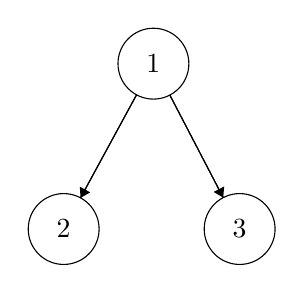
\begin{tikzpicture}[scale=0.15]
\tikzstyle{every node}+=[inner sep=0pt]
\draw [black] (38.9,-25.5) circle (3);
\draw (38.9,-25.5) node {$1$};
\draw [black] (31.3,-39.5) circle (3);
\draw (31.3,-39.5) node {$2$};
\draw [black] (46.2,-39.5) circle (3);
\draw (46.2,-39.5) node {$3$};
\draw [black] (37.47,-28.14) -- (32.73,-36.86);
\fill [black] (32.73,-36.86) -- (33.55,-36.4) -- (32.67,-35.92);
\draw [black] (32.73,-36.86) -- (37.47,-28.14);
%\fill [black] (37.47,-28.14) -- (36.65,-28.6) -- (37.53,-29.08);
\draw [black] (40.29,-28.16) -- (44.81,-36.84);
\fill [black] (44.81,-36.84) -- (44.89,-35.9) -- (44,-36.36);
\draw [black] (44.81,-36.84) -- (40.29,-28.16);
%\fill [black] (40.29,-28.16) -- (40.21,-29.1) -- (41.1,-28.64);
\end{tikzpicture}


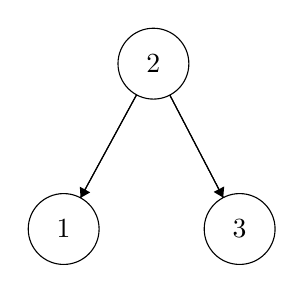
\begin{tikzpicture}[scale=0.15]
\tikzstyle{every node}+=[inner sep=0pt]
\draw [black] (38.9,-25.5) circle (3);
\draw (38.9,-25.5) node {$2$};
\draw [black] (31.3,-39.5) circle (3);
\draw (31.3,-39.5) node {$1$};
\draw [black] (46.2,-39.5) circle (3);
\draw (46.2,-39.5) node {$3$};
\draw [black] (37.47,-28.14) -- (32.73,-36.86);
\fill [black] (32.73,-36.86) -- (33.55,-36.4) -- (32.67,-35.92);
\draw [black] (32.73,-36.86) -- (37.47,-28.14);
%\fill [black] (37.47,-28.14) -- (36.65,-28.6) -- (37.53,-29.08);
\draw [black] (40.29,-28.16) -- (44.81,-36.84);
\fill [black] (44.81,-36.84) -- (44.89,-35.9) -- (44,-36.36);
\draw [black] (44.81,-36.84) -- (40.29,-28.16);
%\fill [black] (40.29,-28.16) -- (40.21,-29.1) -- (41.1,-28.64);
\end{tikzpicture}


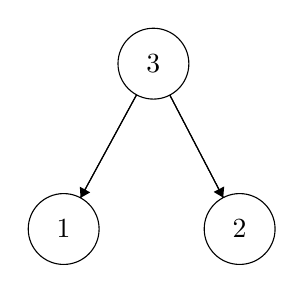
\begin{tikzpicture}[scale=0.15]
\tikzstyle{every node}+=[inner sep=0pt]
\draw [black] (38.9,-25.5) circle (3);
\draw (38.9,-25.5) node {$3$};
\draw [black] (31.3,-39.5) circle (3);
\draw (31.3,-39.5) node {$1$};
\draw [black] (46.2,-39.5) circle (3);
\draw (46.2,-39.5) node {$2$};
\draw [black] (37.47,-28.14) -- (32.73,-36.86);
\fill [black] (32.73,-36.86) -- (33.55,-36.4) -- (32.67,-35.92);
\draw [black] (32.73,-36.86) -- (37.47,-28.14);
%\fill [black] (37.47,-28.14) -- (36.65,-28.6) -- (37.53,-29.08);
\draw [black] (40.29,-28.16) -- (44.81,-36.84);
\fill [black] (44.81,-36.84) -- (44.89,-35.9) -- (44,-36.36);
\draw [black] (44.81,-36.84) -- (40.29,-28.16);
%\fill [black] (40.29,-28.16) -- (40.21,-29.1) -- (41.1,-28.64);
\end{tikzpicture}
\end{center}


This suggests the following marvelous identity, which we will shortly explore:
\begin{equation}\label{ose-eq}
\card{\symn{3}}=\card{\aut{A}}\cdot (\mbox{the number of labeled copies of }A).
\end{equation}

\subsection*{The Orbit-Stabilizer Theorem}

%\begin{definition}
Recall that for every positive integer $k$, we write $[k]$ for $\{1,\ldots,k\}$.
%\end{definition}

\begin{definition}
For every positive integer $k$, we write $\symn{k}$ for the set of bijections from $[k]$ onto $[k]$ (also called the \emph{permutation group on} or the \emph{symmetric group on} $[k]$).
\end{definition}

The names \emph{permutation group} or \emph{symmetric group} emphasize the agebraic nature of \symn{k}. Indeed, we can think of \symn{k}\ as an algebra with a binary operation $\circ$, a unary operation $^{-1}$, and a distinguished element $e$, where, for permutations $f,g\in\symn{k}$, $f\circ g$ is the permutation resulting from the composition of $f$ and $g$, that is, $f\circ g =h$ if and only if for every $i\in [k]$, $h(i) = f(g(i))$; $f^{-1}$ is the permutation which is the inverse of $f$; and $e$ stands for the identity function on $[k]$. With these understandings, you can verify that \symn{k}\ is a group\footnote{These conditions (associativity, identity, inverse, closure) are the axioms for a \emph{group}, which is a fundamental and widely applicable concept in algebra. Group Theory, the part of mathematics which studies groups, is a hugely influential and interesting field. MATH 370 is Penn's introductory group theory course. }: 

\begin{itemize}
\item   
$\circ$ is an associative operation, that is, $(f\circ g)\circ h= f\circ (g\circ h)$, for all $f,g\in\symn{k}$;
\item
 $e$ is an identity with respect to $\circ$, that is, $e\circ f = f\circ e = f$, for all $f\in\symn{k}$; and 
 \item
 $f\circ f^{-1} = f^{-1}\circ f = e$, for all $f\in\symn{k}$.
 \item Permutations are closed under $\circ$, that is, $f \circ g$ is a permutation for all $f, g \in \symn{k}$. 
\end{itemize} 

\begin{aside}
Prove that each of these conditions holds. 
\end{aside}

\begin{definition}
We write $\sgraphn{k}$ ($=\modn{\sg}{k}$) for the set of simple graphs $A$ with $U^A = [k]$.
\end{definition}
\iffalse
\begin{definition}
For each $f\in\symn{k}$ and $A\in\sgraphn{k}$, we define $f[A]$ (called the \emph{image of the graph $A$ under $f$}) to be the graph with universe $[k]$ and edge-set
\[
    L^{f[A]} := \{\op{f(i)}{f(j)} \mid \op{i}{j} \in L^A\}
\]
Note that $f$ is an isomorphism of $A$ onto $f[A]$.
\end{definition}
\fi
Recall that for each $f\in\symn{k}$ and $A\in\sgraphn{k}$, $f[A]$ is the image of the graph $A$ under $f$.
This is an example of a \emph{group action} - the group \symn{k} \emph{acts on} the set \sgraphn{k}\ via the assignment of $f[A]$ to $A$. 

\begin{aside}
    Just as with groups, group actions are axiomatized by a few simple conditions. To verify that this is indeed a group action, show that for all $A\in\sgraphn{k}$ and $f,g\in\symn{k}$ the following properties hold:
    \begin{itemize}
    \item
    $(f\circ g)[A]=f[g[A]]$, and 
    \item
    $e[A]=A$.
    \end{itemize}    
\end{aside}


Recall that \aut{A}\ is the set of automorphisms of $A$. In the current context, for $A\in \sgraphn{k}$, \aut{A}\ is often called the \emph{stabilizer} of $A$, since $f\in\aut{A}$ if and only if $f[A] =A$. 

\begin{definition}
The \emph{orbit of} $A$  under the action of \symn{k}\ (written $\orb{A}{\symn{k}}$) is $\{h[A]\mid h\in\symn{k}\}$. 

In other words, the orbit of $A$ under \symn{k} is the set of $B\in\sgraphn{k}$ such  that $A\cong B$. \end{definition}

The following result is a special case of the \emph{Orbit-Stabilizer Theorem}.
\begin{theorem}\label{orb-stab-thm}
For all $A\in\sgraphn{k}$,
\[
\card{\symn{k}}=\card{\orb{A}{\symn{k}}}\cdot\card{\aut{A}}.
\]
\end{theorem}

\emph{Proof}:
Let $A\in\sgraphn{k}$. We define an equivalence relation $\sim$ on $\symn{k}$: for all $f,g\in\symn{k}$, $f\sim g$ if and only if $(f^{-1}\circ g)\in\aut{A}$. 

\begin{aside}
    Verify that $\sim$ is an equivalence relation, for example, it is reflexive (that is, $f\sim f$), because $f^{-1}\circ f = e$ and $e\in \aut{A}$. Continue and show $\sim$ is symmetric and transitive.
\end{aside}

%To establish the theorem, we prove two lemmata. 

We establish the following two claims about $\sim$ from which the Theorem follows immediately.
\begin{enumerate}
\item
each equivalence class of $\sim$ has size $\card{\aut{A}}$, and
\item
the number of equivalence classes of $\sim$ is $\card{\orb{A}{\symn{k}}}$.
\end{enumerate}
\emph{Ad} claim 1: Fix $f\in\symn{k}$. For each $h\in\aut{A}$ there is a unique $g\in\symn{k}$ such that $f^{-1}\circ g = h$. It follows at once that there is a bijection between $\{g\mid f\sim g\}$ and \aut{A}.

\begin{aside}
    Use the group axioms to first prove that inverses in a group are unique (that is, for any $f$ in a group, there is a unique element $f^{-1}$ such that $f \circ f^{-1} = e = f^{-1} \circ f$, where $e$ is the identity element).

    Using that fact, verify that for each fixed $f, h \in \symn{k}$, there is a unique $g \in \symn{k}$ such that $f^{-1}\circ g = h$. 
\end{aside}

\emph{Ad} claim 2: We show that for every $f,g\in\symn{k}$ $f[A]=g[A]$ if and only if $f\sim g$. We prove each direction of the bi-conditional. 

First, suppose suppose $f\sim g$. Then 
$f^{-1}\circ g \in \aut{A}$. It follows that $(f^{-1}\circ g)[A] = A$ and hence that $f[(f^{-1}\circ g)[A]] = f[A]$. So $(f\circ(f^{-1}\circ g))[A] = f[A]$, and then by associativity $((f\circ f^{-1})\circ g)[A] = f[A]$. As $f \circ f^{-1} = e$, we have $(e\circ g)[A] = f[A]$ from which it follows that $g[A]=f[A]$. 

In the other direction, suppose $f[A]=g[A]$. Then, $f^{-1}[f[A]]=f^{-1}[g[A]]$. Hence, $(f^{-1}\circ f)[A]=(f^{-1}\circ g)[A]$. Hence, $(f^{-1}\circ g)[A]=e[A]= A$. Hence, $f^{-1}\circ g\in \aut{A}$, that is, $f\sim g$. Thus, there is a bijection between the equivalence classes of $\sim$ and $\orb{A}{\symn{k}}$. \qed

We now have the explanation of identity (\ref{ose-eq}), since 
\[
\card{\orb{A}{\symn{k}}}=\mbox{the number of labeled copies of }A.
\]

We illustrate the use of Theorem \ref{orb-stab-thm} via an application to counting structures that satisfy a given schema. %In order to test out our new theorem, %\footnote{Look mom, I got a new Theorem for my birthday! I wanna play with it immediately!} let's use it for some counting. 
Let $S$ be the conjunction of $\sg$ and $\oner$, that is, a graph $A$ satisfies $S$ if and only if $A$ is a 1-regular, simple graph. As we discussed earlier, every such finite graph $A$ has an even number, say $2n$, of nodes; moreover, if $A,B\models S$ and $\card{U^A}=\card{U^B}$, then $A$ is isomorphic to $B$. We will calculate the value of $\modn{S}{2n}$ in two ways - one way using the Orbit-Stabilizer Theorem, and the other directly. 

\subsubsection*{Via the Orbit-Stabilizer Theorem}
Let $A\in\modn{S}{2n}$. As we've just noted above, if $B\in\modn{S}{2n}$, then $A\cong B$. It follows at once that 
\begin{equation}\label{vos-eq}
\modn{S}{2n}=\orb{A}{\symn{2n}}.
\end{equation}
Let's calculate $\card{\aut{A}}$, since Theorem \ref{orb-stab-thm} will then allow us to calculate $\card{\modn{S}{2n}}$. Observe that $A$ consists of $n$ independent edges. Imagine them standing upright and lined up horizontally in some order. 

\begin{center}
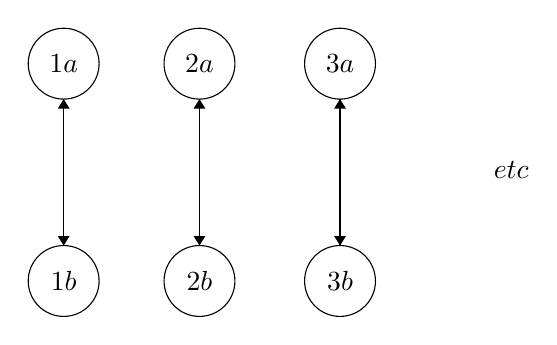
\begin{tikzpicture}[scale=0.15]
\tikzstyle{every node}+=[inner sep=0pt]
\draw [black] (22.2,-16) circle (3);
\draw (22.2,-16) node {$1a$};
\draw [black] (22.2,-34.4) circle (3);
\draw (22.2,-34.4) node {$1b$};
\draw [black] (33.7,-16) circle (3);
\draw (33.7,-16) node {$2a$};
\draw [black] (33.7,-34.4) circle (3);
\draw (33.7,-34.4) node {$2b$};
\draw [black] (45.6,-16) circle (3);
\draw (45.6,-16) node {$3a$};
\draw [black] (45.6,-34.4) circle (3);
\draw (45.6,-34.4) node {$3b$};
\draw (60.1,-25) node {$etc$};
\draw [black] (22.2,-19) -- (22.2,-31.4);
\fill [black] (22.2,-31.4) -- (22.7,-30.6) -- (21.7,-30.6);
\draw [black] (22.2,-31.4) -- (22.2,-19);
\fill [black] (22.2,-19) -- (21.7,-19.8) -- (22.7,-19.8);
\draw [black] (33.7,-19) -- (33.7,-31.4);
\fill [black] (33.7,-31.4) -- (34.2,-30.6) -- (33.2,-30.6);
\draw [black] (33.7,-31.4) -- (33.7,-19);
\fill [black] (33.7,-19) -- (33.2,-19.8) -- (34.2,-19.8);
\draw [black] (45.6,-19) -- (45.6,-31.4);
\fill [black] (45.6,-31.4) -- (46.1,-30.6) -- (45.1,-30.6);
\draw [black] (45.6,-31.4) -- (45.6,-19);
\fill [black] (45.6,-19) -- (45.1,-19.8) -- (46.1,-19.8);
\end{tikzpicture}
\end{center}

Now any permutation of the edges generates an automorphism of $A$. Moreover, in the process of permuting the edges, we have for each edge a choice whether to ``flip'' the edge or not. Since there are $n!$ permutations of the $n$ edges, and $2^n$ choices of which set of edges to flip, there are a total of $n!\cdot 2^n$ automorphisms of $A$. Hence, by Theorem \ref{orb-stab-thm} and equation (\ref{vos-eq}), 
 \[
 \card{\modn{S}{2n}}= (2n)!/n!\cdot 2^n.
 \]

\subsubsection*{Directly}
Here is a second direct method of calculating $\card{\modn{S}{2n}}$ which, thankfully, yields the same result.%\footnote{If it didn't, we'd have to agree that our new toy was broken, and would probably have a miserable rest of the day what with the inconvenience of having to return it and all.}. 
We construct a member $A$ of $\modn{S}{2n}$ as follows. We successively choose the $n$ independent edges that constitute $A$. So for the first edge, we have $\binom{2n}{2}$ choices of a pair of nodes between which to place an edge, and for the second edge, we have $\binom{2n-2}{2}$ choices, .... So the number of ways we can choose a sequence of $n$ independent edges is
\[
\binom{2n}{2}\cdot\binom{2n-2}{2}\cdots\binom{4}{2}\cdot\binom{2}{2}= \frac{(2n)!}{2^n}.
\]
Now any \emph{set} of $n$ edges chosen via this process will appear as the result of $n!$ such sequences of choices; thus, the total number of members of $\modn{S}{2n}$ we can construct is 
\[
\frac{(2n)!}{n!\cdot 2^n}.
\]
\newpage

\subsection{Definability}
Up to this point we have neglected schemata containing free variables. We will now correct this oversight. 

Consider the structure $A$ (which should look familiar) defined by
\[
    U^A = [3], L^A=\{\op{1}{2},\op{1}{3}\}
\]
Define the schema
\[
    S(x):\ \ \ \neg(\exists y)Lyx.
\]
$S(x)$ picks out $1$ uniquely from the structure $A$, because $1$ is the only element in $U^A$ which does not have an incoming edge. Symbolically, we express this as
\[
\{a\in U^A\mid A\models S[x|a]\}=\{1\}.
\]

$S(x)$ expresses the property of having in-degree zero. Since we only consider properties extensionally, we can also say that, in a given structure, $S(x)$ defines the set of nodes of in-degree zero. The concept of definability is central in logic (and many other disciplines). We enshrine it in a definition.

\begin{definition}
Let $S(x)$ be a schema with one free variable $x$ and let $A$ be a structure.
We define $S[A]=\{a\in U^A\mid A\models S[x|a]\}$. In other words, $S[A]$ is the set of nodes $a \in A$ that satisfy the schema $S(x)$ in $A$ when we assign $a$ to the variable $x$. We call $S[A]$ the \emph{set defined by} $S(x)$ in $A$.
\end{definition}

\begin{definition}
We say a set $V\subseteq U^A$ is a \emph{definable subset of} $A$ if and only if there is a schema $S(x)$ such that $S[A]=V$.
\end{definition}

Note that the set $\{2,3\}$ is defined by the schema
\[
S'(x):\ \ \ \neg(\exists y)Lxy.
\]

Are either of the sets $\{2\}$ or $\{3\}$ definable as subsets of $A$? Try as you might, you won't find a schema which picks out either $2$ or $3$ individually. Intuitively, this is because the nodes labelled 2 and 3 appear to be ``indistinguishable from a structural point of view''. Backing up this notion of indistinguishability, we see that the function $h$ mapping 1 to 1, 2 to 3, and 3 to 2, is an automorphism of $A$ which happens to exchange $2$ and $3$. The relevance of this to the question of definability is the content of the following fundamental theorem.

\subsubsection*{The Automorphism Theorem, Orbits, and Definability over finite structures}
\begin{theorem}\label{aut-thm}
Let $A$ be a graph and $h\in\aut{A}$. For every $a\in U^A$ and every schema $S(x)$,
\[
A\models S[x|a]\mbox{ if and only if }A\models S[x|h(a)]. 
\]
\end{theorem}

Theorem \ref{aut-thm} enables us to give a characterization of the definable subsets of finite structures. 
If $f$ is a function with domain $U$ and $V\subseteq U$, we define $f[V]=\{f(a)\mid a\in V\}$ (the $f$ \emph{image} of $V$). With this notation in hand, we can now state a corollary to Theorem \ref{aut-thm} which bears on definability.
\begin{corollary}\label{aut-def-cor}
Let $A$ be a graph and $h\in\aut{A}$. If $V$ is a definable subset of $A$, then $h[V]=V$.
\end{corollary}
Thus, in order to show that $V$ is \emph{not} a definable subset of $A$ it suffices to exhibit an $h\in\aut{A}$ and $a\in V$ such that $h(a)\not\in V$. Moreover, in the case of finite structures, the converse of Corollary \ref{aut-def-cor} is true.
\begin{theorem}\label{fin-aut-def-thm}
Let $A$ be a finite graph and $V\subseteq U^A$. $V$ is a definable subset of $A$, if for every $h\in\aut{A}$, $h[V]=V$.
\end{theorem}

\subsection*{Orbits and Definability over finite structures}
In order to prove Theorem \ref{fin-aut-def-thm}, and to apply it to questions of counting definable sets, the following definitions will be useful. 

\begin{definition}
The \emph{orbit of a node} $a\in U^A$ \emph{under the action of} $\aut{A}$ is the set of all possible images of $a$ under actions $f \in \aut{A}$. Symbolically,
\[
\orb{a}{\aut{A}}=\{h(a)\mid h\in\aut{A}\}.
\]
\end{definition}

\begin{definition}
The \emph{orbits of $A$} is the set of all orbits of individual elements $a \in A$. Symbolically:
\[
    \autorbs{A}=\{\orb{a}{\aut{A}}\mid a\in U^A\}
\]
\end{definition}

As a corollary to Corollary \ref{aut-def-cor} and Theorem \ref{fin-aut-def-thm} we have:
\begin{corollary}\label{def-orbs-cor}
Let $A$ be a finite graph and $V\subseteq U^A$. $V$ is a definable subset of $A$ if and only if either $V=\emptyset$ or there is a sequence of sets $O_1, \ldots,O_k$, where each $O_i\in\autorbs{A}$, and $V = O_1\cup\ldots\cup O_k$.
\end{corollary}

\begin{aside}
    Use Corollary \ref{aut-def-cor} and Theorem \ref{fin-aut-def-thm} to prove this. 
\end{aside}

It follows at once from Corollary \ref{def-orbs-cor}, that if $A$ is a finite graph, then the number of definable subsets of $A$ is $2^{\card{\autorbs{A}}}$. 



\subsubsection*{An example: definable subsets of simple graphs with four nodes}

To make this all a little bit more concrete, lets give a complete analysis of the definable subsets of simple graphs with four nodes.

Let's classify all members of $\modn{\sg}{4}$ up to isomorphism - that is, exhibit examples of all the size-4 simple graphs. There is a single such graph with no edges which we will call $A_1$. This looks like

\[
    \begin{array}{|l|}
    \hline
    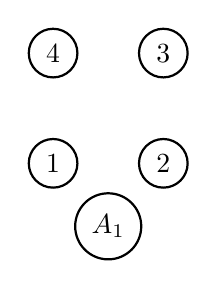
\begin{tikzpicture}
[scale=.2]
\begin{scope}[every node/.style={circle,thick,draw}]
    \node (1) at (0,4) {1};
    \node (2) at (7,4) {2};
    \node (3) at (7,11) {3};
    \node (4) at (0,11) {4};
   \node(A) at (3.5,0) {$A_1$};
\end{scope}
\end{tikzpicture}\\
\hline
\end{array}
\]

By symmetry, there is also a single maximal size-4 graph with 6 edges

\[
    \begin{array}{|l|}
    \hline
    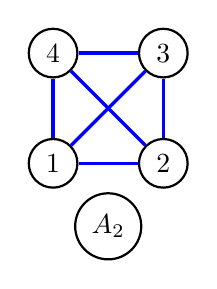
\begin{tikzpicture}
[scale=.2]
\begin{scope}[every node/.style={circle,thick,draw}]
    \node (1) at (0,4) {1};
    \node (2) at (7,4) {2};
    \node (3) at (7,11) {3};
    \node (4) at (0,11) {4};
   \node(A) at (3.5,0) {$A_2$};
\end{scope}

\begin{scope}[%>={Stealth[black]},
              every node/.style={fill=white,circle},
              every edge/.style={draw=blue,very thick}]
     \draw (1) edge  (2);
     \draw (2) edge  (3);
     \draw (3) edge  (4);
     \draw (4) edge  (1);
     \draw (4) edge  (2);
     \draw (3) edge  (1);
             
\end{scope}
\end{tikzpicture}\\
\hline
\end{array}
\]

Up to isomorphism, there is one size-4 graph with a single edge (since we only care about equivalence up to isomorphism, the labels of the ends of the single edge don't matter). By symmetry, there is a single size-4 graph with 5 edges. 

\[
    \begin{array}{|l|l|}
        \hline
        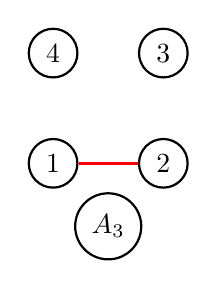
\begin{tikzpicture}
        [scale=.2]
        \begin{scope}[every node/.style={circle,thick,draw}]
            \node (1) at (0,4) {1};
            \node (2) at (7,4) {2};
            \node (3) at (7,11) {3};
            \node (4) at (0,11) {4};
           \node(A) at (3.5,0) {$A_3$};
        \end{scope}

        \begin{scope}[%>={Stealth[black]},
                      every node/.style={fill=white,circle},
                      every edge/.style={draw=red,very thick}]
              \draw (1) edge  (2);
             %\draw (2) edge  (3);
             %\draw (3) edge  (4);
             %\draw (4) edge  (1);
             %\draw (4) edge  (2);
             %\draw (3) edge  (1);             
        \end{scope}
        \end{tikzpicture}
        &
        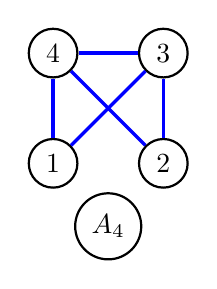
\begin{tikzpicture}
        [scale=.2]
        \begin{scope}[every node/.style={circle,thick,draw}]
            \node (1) at (0,4) {1};
            \node (2) at (7,4) {2};
            \node (3) at (7,11) {3};
            \node (4) at (0,11) {4};
           \node(A) at (3.5,0) {$A_4$};
        \end{scope}

        \begin{scope}[%>={Stealth[black]},
                      every node/.style={fill=white,circle},
                      every edge/.style={draw=blue,very thick}]
             %\draw (1) edge  (2);
             \draw (2) edge  (3);
             \draw (3) edge  (4);
             \draw (4) edge  (1);
             \draw (4) edge  (2);
             \draw (3) edge  (1);
                     
        \end{scope}
        \end{tikzpicture}\\
        \hline
    \end{array}
\]

There are two non-isomorphic size-4 graphs with two edges, and similarly two such graphs with 4 edges. 

\[
    \begin{array}{|l|l|}
    \hline

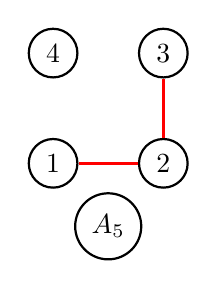
\begin{tikzpicture}
[scale=.2]
\begin{scope}[every node/.style={circle,thick,draw}]
    \node (1) at (0,4) {1};
    \node (2) at (7,4) {2};
    \node (3) at (7,11) {3};
    \node (4) at (0,11) {4};
   \node(A) at (3.5,0) {$A_5$};
\end{scope}

\begin{scope}[%>={Stealth[black]},
              every node/.style={fill=white,circle},
              every edge/.style={draw=red,very thick}]
\draw (1) edge  (2);
     \draw (2) edge  (3);
     %\draw (3) edge  (4);
     %\draw (4) edge  (1);
     %\draw (4) edge  (2);
     %\draw (3) edge  (1);             
\end{scope}
\end{tikzpicture}
&
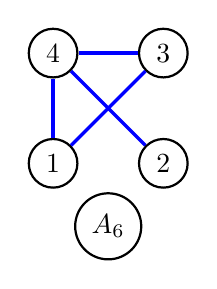
\begin{tikzpicture}
[scale=.2]
\begin{scope}[every node/.style={circle,thick,draw}]
    \node (1) at (0,4) {1};
    \node (2) at (7,4) {2};
    \node (3) at (7,11) {3};
    \node (4) at (0,11) {4};
   \node(A) at (3.5,0) {$A_6$};
\end{scope}

\begin{scope}[%>={Stealth[black]},
              every node/.style={fill=white,circle},
              every edge/.style={draw=blue,very thick}]
%\draw (1) edge  (2);
%     \draw (2) edge  (3);
     \draw (3) edge  (4);
     \draw (4) edge  (1);
     \draw (4) edge  (2);
     \draw (3) edge  (1);
             
\end{scope}
\end{tikzpicture}
\\
\hline
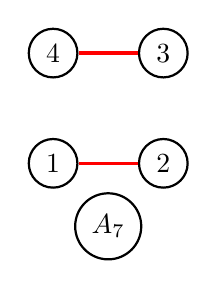
\begin{tikzpicture}
[scale=.2]
\begin{scope}[every node/.style={circle,thick,draw}]
    \node (1) at (0,4) {1};
    \node (2) at (7,4) {2};
    \node (3) at (7,11) {3};
    \node (4) at (0,11) {4};
   \node(A) at (3.5,0) {$A_7$};
\end{scope}

\begin{scope}[%>={Stealth[black]},
              every node/.style={fill=white,circle},
              every edge/.style={draw=red,very thick}]
\draw (1) edge  (2);
     %\draw (2) edge  (3);
     \draw (3) edge  (4);
     %\draw (4) edge  (1);
     %\draw (4) edge  (2);
     %\draw (3) edge  (1);             
\end{scope}
\end{tikzpicture}
&
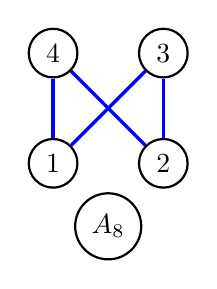
\begin{tikzpicture}
[scale=.2]
\begin{scope}[every node/.style={circle,thick,draw}]
    \node (1) at (0,4) {1};
    \node (2) at (7,4) {2};
    \node (3) at (7,11) {3};
    \node (4) at (0,11) {4};
   \node(A) at (3.5,0) {$A_8$};
\end{scope}

\begin{scope}[%>={Stealth[black]},
              every node/.style={fill=white,circle},
              every edge/.style={draw=blue,very thick}]
%\draw (1) edge  (2);
     \draw (2) edge  (3);
%     \draw (3) edge  (4);
     \draw (4) edge  (1);
     \draw (4) edge  (2);
     \draw (3) edge  (1);
     \end{scope}
\end{tikzpicture}

    \\
    \hline
    \end{array}
\]

Lastly, there are three non-isomorphic size-4 simple graphs with three edges. $A_9$ and $A_{10}$ are complements of each other, whereas $A_{11}$, is its own complement. 

\[
    \begin{array}{|l|l|l|}
    \hline
    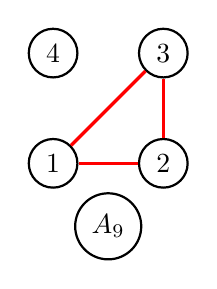
\begin{tikzpicture}
[scale=.2]
\begin{scope}[every node/.style={circle,thick,draw}]
    \node (1) at (0,4) {1};
    \node (2) at (7,4) {2};
    \node (3) at (7,11) {3};
    \node (4) at (0,11) {4};
   \node(A) at (3.5,0) {$A_9$};
\end{scope}

\begin{scope}[%>={Stealth[black]},
              every node/.style={fill=white,circle},
              every edge/.style={draw=red,very thick}]
\draw (1) edge  (2);
     \draw (2) edge  (3);
%     \draw (3) edge  (4);
%     \draw (4) edge  (1);
%     \draw (4) edge  (2);
     \draw (3) edge  (1);
     \end{scope}
\end{tikzpicture}
&
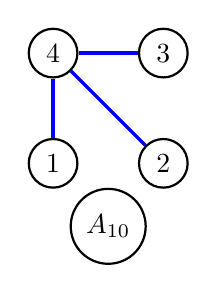
\begin{tikzpicture}
[scale=.2]
\begin{scope}[every node/.style={circle,thick,draw}]
    \node (1) at (0,4) {1};
    \node (2) at (7,4) {2};
    \node (3) at (7,11) {3};
    \node (4) at (0,11) {4};
   \node(A) at (3.5,0) {$A_{10}$};
\end{scope}

\begin{scope}[%>={Stealth[black]},
              every node/.style={fill=white,circle},
              every edge/.style={draw=blue,very thick}]
%\draw (1) edge  (2);
%     \draw (2) edge  (3);
     \draw (3) edge  (4);
     \draw (4) edge  (1);
     \draw (4) edge  (2);
%     \draw (3) edge  (1);
             
\end{scope}
\end{tikzpicture}
&
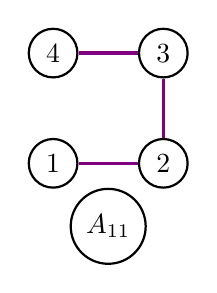
\begin{tikzpicture}
[scale=.2]
\begin{scope}[every node/.style={circle,thick,draw}]
    \node (1) at (0,4) {1};
    \node (2) at (7,4) {2};
    \node (3) at (7,11) {3};
    \node (4) at (0,11) {4};
   \node(A) at (3.5,0) {$A_{11}$};
\end{scope}

\begin{scope}[%>={Stealth[black]},
              every node/.style={fill=white,circle},
              every edge/.style={draw=violet,very thick}]
 \draw (1) edge  (2);
     \draw (2) edge  (3);
     \draw (3) edge  (4);
%     \draw (4) edge  (1);
 %    \draw (4) edge  (2);
  %   \draw (3) edge  (1);
     \end{scope}
\end{tikzpicture}
\\
\hline

\end{array}
\]

\begin{aside}
    Verify that these are all of the non-isomorphic graphs of size 4 by beginning with 4 empty nodes and iteratively constructing all non-isomorphic graphs with increasing number of edges. 
\end{aside}

Now that we have a maximal collection of pairwise non-isomorphic graphs in $\modn{\sg}{4}$, we can calculate $\card{\orb{A_i}{\symn{4}}}$ and $\card{\aut{A_i}}$ for each $1\leq i\leq 11$. 

\begin{aside}
    Prove that $\aut{A} = \aut{A^c}$ for every simple graph $A$. 

    From this, it follows that if $A_i$ and $A_j$ are complements, we have that $\card{\aut{A_i}} = \card{\aut{A_j}}$ and moreover $\card{\orb{A_i}{\symn{4}}} = \card{\orb{A_j}{\symn{4}}}$. This will make our counting easier, because it nearly halves the amount of work we have to do. 
\end{aside}

What is $\card{\orb{A_1}{\symn{4}}}$, or in other words, how many distinct ways can we place 0 edges onto 4 labelled nodes? There is only one way to do this, so $\card{\orb{A_1}{\symn{4}}} = 1$. What is $\card{\aut{A_1}}$, or in other words, how many ways can we permute the edges of $A_1$ once the edges are fixed in place? There are no edges, so any permutation of the nodes (of which there are $4! = 24$) is valid. It follows that $\card{\aut{A_1}} = 24$. By symmetry, it follows that $\card{\orb{A_2}{\symn{4}}} = 1$ and $\card{\aut{A_2}} = 24$ as well. 

As another example, let's calculate $\card{\orb{A_5}{\symn{4}}}$ and $\card{\aut{A_5}}$ (and hence the values for $A_6$ as well). There are $4 \cdot 3 = 12$ ways of placing 2 edges onto 4 nodes such that the two edges are connected as in $A_5$, as there are $4$ choices for the ``central'' node and $\binom{3}{2} = 3$ choices for which two other nodes (which we will call \emph{leaves}) get connected to the central node. It follows that $\card{\orb{A_5}{\symn{4}}} = \card{\orb{A_6}{\symn{4}}} = 12$. Once the edges have been fixed, there are two possible automorphisms: the identity automorphism, and automorphism which exchanges the two leaf nodes. It follows that $\card{\aut{A_5}} = \card{\aut{A_6}} = 2$. 

Without too much extra work, we arrive at the complete table:

\[
\begin{array}{|c|c|c|}
\hline
A_i  & \card{\orb{A_i}{\symn{4}}} & \card{\aut{A_i}}\\
\hline
A_1 & 1 & 24\\
\hline
A_2 & 1 & 24 \\
\hline
A_3 & 6 & 4\\
\hline
A_4 & 6 & 4\\
\hline
A_5 & 12 & 2\\
\hline
A_6 & 12 & 2\\
\hline
A_7 & 3 & 8 \\
\hline
A_8 & 3 & 8 \\
\hline
A_9 & 4 & 6 \\
\hline
A_{10} & 4 & 6 \\
\hline
A_{11} & 12 & 2\\
\hline
\end{array}
\]

\begin{aside}
    Calculate each of the values not discussed in the examples. 
\end{aside}

Note the ``verification'' of the result predicted by the Orbit-Stabilizer Theorem: $\card{\orb{A_i}{\symn{4}}} \cdot \card{\aut{A_i}} = \card{\symn{4}} (= 24)$.
%\subsection{Addendum}

By Corollary \ref{def-orbs-cor}, calculating $\autorbs{A_i}$ suffices to determine which sets are definable in each $A_i$. 

\begin{example}
What is $\autorbs{A_5}$?
\end{example}
To determine $\autorbs{A_5}$, it suffices to determine the orbits of individual elements. The orbit of node $4$ is $\{4\}$, as it is the only isolated node. The orbit of $2$ is $\{2\}$, as it is the only node of degree two. The orbit of $1$ is $\{1, 3\}$ as $1$ is a leaf node, and we had an automorphism that exchanged leaf nodes. As the set of orbits partition the nodes, the orbit of $3$ is $\{1, 3\}$ as well. It follows that $\autorbs{A_5} = \{\{2\}, \{4\}, \{1, 3\}\}$. 

\begin{aside}
A \emph{partition} of a set $S$ is a collection $\mathcal{P}$ of subsets of $S$ such that: (1) every $s \in S$ is in some $P \in \mathcal{P}$, and (2) if $P, P' \in \mathcal{P}$ and $P \cap P' \neq 0$, then $P = P'$ (ie, no distinct elements of $\mathcal{P}$ overlap).

$\autorbs{A}$ trivially satisfies condition (1), since every node in $A$ is in its own orbit. Complete the proof $\autorbs{A}$ is a partition of the nodes of $A$ by showing that condition (2) holds. 
\end{aside}  

With a little more work, we arrive at the following table. 
\[
\begin{array}{l l}
A_i & \autorbs{A_i}\\
\hline
A_1, A_2 & \{[4]\}\\
A_3, A_4 & \{\{1,2\},\{3,4\}\}\\
A_5, A_6 & \{\{2\},\{4\},\{1,3\}\}\\
A_7, A_8 & \{[4]\}\\
A_9, A_{10} & \{\{1,2,3\},\{4\}\}\\
A_{11} & \{\{1,4\},\{2,3\}\}
\end{array}
\]

\begin{aside}
    Derive each of the above sets of orbits yourself, to make sure all the concepts fit into place. 
\end{aside}

\subsection*{Proofs for Theorem \ref{aut-thm} and Theorem \ref{fin-aut-def-thm}}
We now develop the necessary technology in order to give proof sketches for Theorem \ref{aut-thm} and Theorem \ref{fin-aut-def-thm}.  

\subsubsection*{Automorphisms and Degree}
Let $A$ be a graph and $a\in U^A$. Recall that the \emph{neighborhood of} $a$ in $A$ is $\nbh{a}{A} := \{b\in U^A\mid\op{a}{b}\in L^A\}$. The \emph{degree of} $a$ in $A$ is $\dg{a}{A} := \card{\{b\in U^A\mid\op{a}{b}\in L^A\}}$. We have the following fact:
\begin{proposition}
For every graph $A$, $a\in U^A$, and $h\in\aut{A}$,
\[
h[\nbh{a}{A}]=\nbh{h(a)}{A}.
\]
Hence,
\[
\dg{a}{A} = \dg{h(a)}{A}. 
\]
In other words, automorphisms preserve degree. 
\end{proposition}

\begin{aside}
    Show that this follows from the definition of an automorphism.
\end{aside}

\begin{definition}
    We say that a graph $A$ is \emph{rigid} if and only if $\aut{A}=\{e\}$, that is, $A$ has no non-trivial automorphisms.
\end{definition}

It follows at once from Theorem \ref{fin-aut-def-thm} that if $A$ is a finite rigid structure and $V\subseteq U^A$, then $V\in\Def{A}$.

\begin{aside}
    Why? Think about what $\aut{A}=\{e\}$ implies about the orbit of each element (and hence $\autorbs{A}$). 
\end{aside}

\begin{aside}
    No member of $\modn{\sg}{4}$ is rigid, as each has non-trivial automorphisms. This suggests an interesting question: ``what is the least $n$ such that $\modn{\sg}{n}$ contains a rigid graph?''
\end{aside}

\subsubsection*{Proof Sketch of Theorem \ref{fin-aut-def-thm}}
We aim to show that for every finite graph $A$, $V \subset A$ is definable iff every automorphism $h \in \aut{A}$ leaves $V$ unchanged. The generalization to structures interpreting multiple polyadic predicates is straightforward.

First, suppose $A$ is a finite graph, $a\in U^A$, and $V=\orb{A}{\aut{A}}$. We construct a schema $S(x)$ such that $S[A]=V$ by . We may suppose without loss of generality that $U^A=[k]$ for some $k\in\mathbb{Z}^+$ and that $a=1$. For each $1\leq i,j\leq k$, let the schema $S_{i,j}$ be $Lx_ix_j$ if $\op{i}{j}\in L^A$, and $\neg Lx_ix_j$ otherwise. Let $S(x)$ be the schema
\[
(\exists x_2)\ldots(\exists x_k)(\bigwedge_{1\leq i,j\leq k}S_{i,j}\wedge\bigwedge_{1\leq i<j\leq k}x_i\neq x_j\wedge(\forall y)\bigvee_{1\leq i\leq k} y=x_i).
\] 
Let $a_1,\dots,a_k$ be a sequence of nodes from $U^A$ and observe that
\[
A\models(\bigwedge_{1\leq i,j\leq k}S_{i,j}\wedge\bigwedge_{1\leq i<j\leq k}x_i\neq x_j\wedge(\forall y)\bigvee_{1\leq i\leq k} y=x_i)[(x_1|a_1),\ldots,(x_k|a_k)]
\]
if and only if the function mapping $i$ to $a_i$ is an automorphism of $A$. \qed


Theorem \ref{aut-thm} is a corollary of the following more general result concerning isomorphisms of structures.
\begin{theorem}\label{iso-thm}
Suppose $A$ and $B$ are structures and $f$ is an isomorphism of $A$ onto $B$. Then for every schema $S(x_1,\ldots,x_k)$ and sequence of elements $a_1,\dots,a_k\in U^A$,
\begin{equation}\label{iso-eq}
A\models S[(x_1|a_1),\ldots,(x_k|a_k)]\mbox{ iff }B\models S[(x_1|f(a_1)),\ldots,(x_k|f(a_k))].
\end{equation}
\end{theorem}

{\bf Proof sketch of Theorem \ref{iso-thm}}:
We give the argument for graphs; the generalization to structures interpreting multiple polyadic predicates is straightforward.
The argument proceeds by induction on the syntactic structure of schemata. The base case verifies (\ref{iso-eq}) for atomic schemata, that is, schemata of the form $Lx_ix_j$ or $x_i=x_j$, for some $i,j$. In this case, the verification follows directly from the hypothesis that $f$ is an isomorphism from $A$ onto $B$, in particular, that it is edge-preserving and injective.

Suppose $S$ is a truth-functional combination, for example the conjunction, of schemata $S'$ and $S''$, where, as hypothesis of induction, (\ref{iso-eq}) holds for both $S'$ and $S''$. Then,
\[
\begin{array}{lc}
A\models S[(x_1|a_1),\ldots,(x_k|a_k)] & \mbox{ iff}\\
A\models S'[(x_1|a_1),\ldots,(x_k|a_k)]\mbox{ and }A\models S''[(x_1|a_1),\ldots,(x_k|a_k)] & \mbox{ iff}\\
B\models S'[(x_1|f(a_1)),\ldots,(x_k|f(a_k))]\mbox{ and }B\models S''[(x_1|f(a_1)),\ldots,(x_k|f(a_k))] & \mbox{ iff}\\
B\models S[(x_1|f(a_1)),\ldots,(x_k|f(a_k))].
\end{array}
\]
The first and third biconditionals follow from the truth-functional semantics of conjunction, while the second follows from the induction hypothesis.

Finally, suppose that $S$ is $(\exists y)S'(x_1,\ldots,x_k,y)$ and (\ref{iso-eq}) holds for $S'$ (the universal quantifier is handled similarly). Then,
\[
\begin{array}{lc}
A\models S[(x_1|a_1),\ldots,(x_k|a_k)] & \mbox{ iff}\\
\mbox{for some $a\in U^A$ }
A\models S'[(x_1|a_1),\ldots,(x_k|a_k),(y|a)] & \mbox{ iff}\\
\mbox{for some $a\in U^A$ }
B\models S'[(x_1|f(a_1)),\ldots,(x_k|f(a_k)),(y|f(a))] & \mbox{ iff}\\
\mbox{for some $b\in U^B$ }
B\models S'[(x_1|f(a_1)),\ldots,(x_k|f(a_k)),(y|b)] & \mbox{ iff}\\
B\models S[(x_1|f(a_1)),\ldots,(x_k|f(a_k))].
\end{array}
\]
The first and fourth biconditionals follow from the semantics for the existential quantifier, the second from the induction hypothesis, and the third from the hypothesis that $f$ is an isomorphism from $A$ onto $B$, in particular, that it is
surjective. \qed 

\begin{aside}
    In the proof above, the only truth-functional connective we considered was conjunction. The other cases are handled similarly. Complete those cases yourself, either by writing out the whole argument, or by showing that a conditional can be defined in terms of some conditionals whose cases you already worked out (for example, each of the connectives can be defined in terms of $\lnot$ and $\land$, so those two cases suffice). 
\end{aside}

\begin{aside}
    Show that Theorem \ref{aut-thm} is a corollary to Theorem \ref{iso-thm}
\end{aside}

\subsection*{Definability in Infinite Structures}
We now turn away from the safe confines of the finite and present two examples pertaining to definability in infinite structures.

\subsubsection*{A Structure With Many Automorphisms: The Integers with Absolute Value}
Let $A$ be an infinite graph defined by
\[
    U^A = \mathbb{Z}, L^A = \{\op{i}{j}\mid j \mbox{ is the absolute value of } i\}
\]
(Recall that the absolute value of an integer $i$ is $i$, if $i\geq 0$, and is $-i$, if $i< 0$.) 

\begin{center}
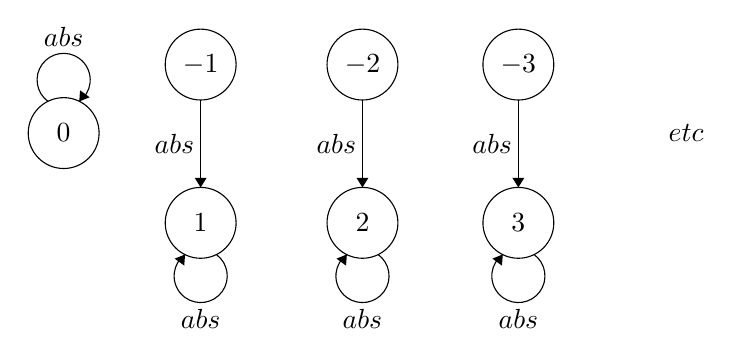
\begin{tikzpicture}[scale=0.15]
\tikzstyle{every node}+=[inner sep=0pt]
\draw [black] (14.4,-29.1) circle (3);
\draw (14.4,-29.1) node {$0$};
\draw [black] (26,-23.3) circle (3);
\draw (26,-23.3) node {$-1$};
\draw [black] (26,-36.7) circle (3);
\draw (26,-36.7) node {$1$};
\draw [black] (39.7,-23.3) circle (3);
\draw (39.7,-23.3) node {$-2$};
\draw [black] (39.7,-36.7) circle (3);
\draw (39.7,-36.7) node {$2$};
\draw [black] (52.9,-23.3) circle (3);
\draw (52.9,-23.3) node {$-3$};
\draw [black] (52.9,-36.7) circle (3);
\draw (52.9,-36.7) node {$3$};
% \draw [black] (67.1,-29.1) circle (3);
\node at (67.1,-29.1) {$etc$};
\draw [black] (13.077,-26.42) arc (234:-54:2.25);
\draw (14.4,-21.85) node [above] {$abs$};
\fill [black] (15.72,-26.42) -- (16.6,-26.07) -- (15.79,-25.48);
\draw [black] (26,-26.3) -- (26,-33.7);
\fill [black] (26,-33.7) -- (26.5,-32.9) -- (25.5,-32.9);
\draw (25.5,-30) node [left] {$abs$};
\draw [black] (27.323,-39.38) arc (54:-234:2.25);
\draw (26,-43.95) node [below] {$abs$};
\fill [black] (24.68,-39.38) -- (23.8,-39.73) -- (24.61,-40.32);
\draw [black] (39.7,-26.3) -- (39.7,-33.7);
\fill [black] (39.7,-33.7) -- (40.2,-32.9) -- (39.2,-32.9);
\draw (39.2,-30) node [left] {$abs$};
\draw [black] (41.023,-39.38) arc (54:-234:2.25);
\draw (39.7,-43.95) node [below] {$abs$};
\fill [black] (38.38,-39.38) -- (37.5,-39.73) -- (38.31,-40.32);
\draw [black] (54.223,-39.38) arc (54:-234:2.25);
\draw (52.9,-43.95) node [below] {$abs$};
\fill [black] (51.58,-39.38) -- (50.7,-39.73) -- (51.51,-40.32);
\draw [black] (52.9,-26.3) -- (52.9,-33.7);
\fill [black] (52.9,-33.7) -- (53.4,-32.9) -- (52.4,-32.9);
\draw (52.4,-30) node [left] {$abs$};
\end{tikzpicture}
\end{center}


Every permutation $g$ of $\mathbb{Z}^+$ can be extended to an automorphism $h$ of $A$ by setting $h(i)=g(i)$, for $i\in \mathbb{Z}^+$; $h(0)=0$; and $h(i)=-g(-i)$, for $i<0$. 

\begin{aside}
    Why is this? The only relation we have in our graph is the absolute-value relation, so our graph looks like a bunch of pairs $n, -n$ (for $n$ positive) where there is an edge from $-n$ to $n$ and an edge from $n$ to $n$ (ie a self-loop at $n$), plus $0$ all on its own with a self-loop. So long as we keep $0$ fixed in place, permuting any of our $(n, -n)$-pairs gives us an automorphism, provided that we match don't ``flip'' any of the pairs - ie, negative numbers (which have in-degree 0) map to negative numbers, and positive numbers (which have in-degree 2) map to positive numbers. The formulae mentioned above ensure that this happens. 
\end{aside}



Let's write $\mathbb{Z}^-$ for the set of negative integers. Thus, $\autorbs{A}= \{\mathbb{Z}^+,\{0\},\mathbb{Z}^-\}$. Each orbit of $\aut{A}$ acting on $U^A$ is definable:
\begin{itemize}
\item 
$S_1[A] = \mathbb{Z}^+$, where $S_1(x)$ is $(\exists y)(y\neq x \wedge Lyx)$;
\item 
$S_2[A] = \mathbb{Z}^-$, where $S_2(x)$ is $(\forall y)\neg Lyx$;
\item 
$S_3[A] = \{0\}$, where $S_3(x)$ is $\neg S_1(x)\wedge\neg S_2(x)$.
\end{itemize} 

\begin{aside}
    $S_1[A] = \mathbb{Z}^+$ as the positive integers are the only ones which have in-neighbours distinct from themselves (because there is an edge from a negative integer to its positive absolute value). Explain in your own words why $S_2[A] = \mathbb{Z}^-$ and $S_3[A] = \{0\}$. 
\end{aside}

By Corollary \ref{def-orbs-cor}, it follows that there are exactly eight sets definable in $A$:
\begin{enumerate}
\item $\emptyset$,
\item $\{0\}$,
\item $\mathbb{Z}^+$,
\item $\mathbb{Z}^-$,
\item $\mathbb{Z}^+\cup\mathbb{Z}^-$,
\item $\mathbb{Z}^+\cup\{0\}$,
\item $\mathbb{Z}^-\cup\{0\}$,
\item $\mathbb{Z}$.
\end{enumerate}

\subsubsection*{Defining Infinite Graphs Themselves}
We've just figured out which subsets of $A$ are definable, but what about $A$ itself - ie, can $A$ be uniquely specified by some schema?

The situation would be simpler if we had a finite graph.
\begin{theorem}
If $D$ is a finite graph, then there is a schema $S$ such that for every graph $D'$, 
\[
D'\models S \mbox{ if and only if } D'\cong D.
\]
\end{theorem}

\begin{aside}
    Give a proof of this theorem. Intuitively, the idea is that if a graph is finite, you only need to specify finitely many things about it (eg how many nodes there are, which nodes are connected by edges) in order to uniquely pick out the graph. 
\end{aside}

In sharp contrast, the following theorem shows that \emph{no} infinite structure can be perfectly described by any schema. In order to state the result, we need to define $\theo{D}$, the \emph{complete theory of} $D$:
\[
\theo{D} = \{S\mid S \mbox{ is a schema and } D\models S\}. 
\]
\begin{theorem}\label{infnotcat-thm}
For every infinite graph $D$, there is a graph $D'$, $D'\models\theo{D}$ and $D'\not\cong D$.
\end{theorem}
Theorem \ref{infnotcat-thm} is a corollary to the Compactness Theorem for PQT, a fundamental\footnote{By many accounts, this is \emph{the} most fundamental result about First-Order Logic (the common name for what we call PQT).} result we will study shortly.

\subsubsection*{A Rigid Structure: The Natural Numbers with Successor}
We now look at another infinite structure $B$ where definability behaves very differently. $B$ is described by:
\[
    U^B = \mathbb{N}, L^B = \{\op{i}{j}\mid j=i+1\}
\]

\begin{center}
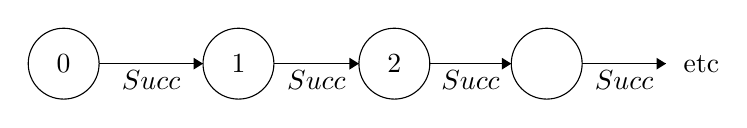
\begin{tikzpicture}[scale=0.15]
\tikzstyle{every node}+=[inner sep=0pt]
\draw [black] (12,-29.5) circle (3);
\draw (12,-29.5) node {$0$};
\draw [black] (26.8,-29.5) circle (3);
\draw (26.8,-29.5) node {$1$};
\draw [black] (40,-29.5) circle (3);
\draw (40,-29.5) node {$2$};
\draw [black] (52.9,-29.5) circle (3);
% \draw (52.9,-29.5) node {$3$};
\node at (66,-29.5) {etc};
\draw [black] (15,-29.5) -- (23.8,-29.5);
\fill [black] (23.8,-29.5) -- (23,-29) -- (23,-30);
\draw (19.4,-30) node [below] {$Succ$};
\draw [black] (29.8,-29.5) -- (37,-29.5);
\fill [black] (37,-29.5) -- (36.2,-29) -- (36.2,-30);
\draw (33.4,-30) node [below] {$Succ$};
\draw [black] (43,-29.5) -- (49.9,-29.5);
\fill [black] (49.9,-29.5) -- (49.1,-29) -- (49.1,-30);
\draw (46.45,-30) node [below] {$Succ$};
\draw [black] (55.9,-29.5) -- (63,-29.5);
\fill [black] (63,-29.5) -- (62.2,-29) -- (62.2,-30);
\draw (59.45,-30) node [below] {$Succ$};
\end{tikzpicture}
\end{center}

A first observation is that $\aut{B}=\{e\}$, that is, $B$ is a rigid structure. Intuitively, any homomorphism must map $0$ to itself, since it is the only element which doesn't have anything less than it. Similary, any homomorphism must map any positive $n$ to itself, since $n$ is the only number with exactly $n - 1$ predecessors. 

We can establish this formally by mathematical induction. Suppose $h$ is an automorphism of $B$. Since $0$ is the only node of $B$ with in-degree $0$, we must have $h(0)=0$. Now suppose, as induction hypothesis, that $h(n)=n$. Since $n+1$ is the only member of $U^B$ to which $n$ is related, it follows from the hypothesis that $h$ is an automorphism that $h(n+1)=n+1$. It follows that for all $k\in U^B$, $h(k)=k$. Hence, $\aut{B}=\{e\}$. 

This argument suggests that for every $k\in U^B$, $\{k\}$ is definable over $B$. Let's show this, again by induction. First, the schema $S^0(x): (\forall y)\neg Lyx$ defines $\{0\}$ over $B$. Next, as induction hypothesis, suppose that $S^n(x)$ defines $\{n\}$ over $B$. Let $z$ be a variable which does not occur anywhere in $S^n(x)$ and let $S^n(z)$ be the result of replacing $x$ with $z$ at all its occurrences in $S^n(x)$. Then the schema $(\exists z)(S^n(z)\wedge Lzx)$ defines $\{n+1\}$ over $B$. this completes the induction and establishes that for every $k\in U^B$, $\{k\}$ is definable over $B$. It follows at once that every finite subset of $U^B$ and every co-finite subset of $U^B$ is definable over $B$. 

\begin{aside}
    Why is it important that $z$ be a variable which occurs nowhere in $S^n(x)$?
\end{aside}

What other subsets of $U^B$ are definable over $B$? Note that since $B$ is rigid, there is no possibility of exhibiting an automorphism $h$ of $B$ with $h[X]\neq X$, that is, the ``automorphism method'' is powerless to establish the undefinability of any subset of $U^B$ in $B$. Could it be that every subset of $U^B$ is definable over $B$? 




\newpage

\subsection{Undefinability}
\subsubsection*{Cantor's Theorem and Cardinality Arguments}
We will show that for every infinite structure $C$ there is a subset $X\subseteq U^C$ which is \emph{not} definable over $C$. This result is a corollary to the celebrated Cantor Diagonal Theorem.
\begin{theorem}[Cantor]\label{cantordiag-thm}
Let $U$ be an infinite set and let $V_1, V_2, \ldots$ be a sequence of subsets of $U$. There is subset $W$ of $U$ such that for all $i\geq 1$, $W\neq V_i$.
\end{theorem}
\emph{Proof}: Suppose $U$ is an infinite set. Let $U^*= \{a_1, a_2, \ldots\}$ be a countably infinite subset of $U$ and let $V_1, V_2, \ldots$ be a sequence of subsets of $U$. Let $W=\{i\mid a_i\not\in V_i\}$. Note that for every $i$, $a_i\in W$ if and only if $a_i\not\in V_i$. It follows that for all $i$, $W\neq V_i$. \qed

\begin{aside}
    The idea in the above proof is to show that, regardless of which way we list the subsets $V_i$ of $U$, there will always be some other subset $W$ of $U$ which is not in the list. We construct $W$ by making sure it differs from each $V_i$ by at least one element; to do this, it suffices to let $a_i \in W$ iff $a_i \not \in V_i$. 
\end{aside}

In order to apply Theorem \ref{cantordiag-thm} to questions about definable sets we require the following result.
\begin{theorem}\label{countschema-thm}
For every structure $C$, there is a sequence $V_1,V_2,\ldots$ of subsets of $U^C$ such that for every set $X$ definable over $C$, there is an $i$ such that $X=V_i$. 

For those who know a little bit of set theory, this says that there are only countably many definable subsets of any given structure.
\end{theorem}
\emph{Proof}: Every schema is a finite sequence of symbols drawn from a finite alphabet. Thus, we may arrange all schemata $S(x)$ in a list $S_1(x), S_2(x),\ldots$, first ordered by length, and then within length, alphabetically. We obtain a list $V_1,V_2,\ldots $ of all the sets definable over $C$ by setting $V_i=S_i[C]$ for all $i$. \qed

As Theorems \ref{cantordiag-thm} and Theorem \ref{countschema-thm} entails that we can list all definable subsets of an infinite structure $C$, and theorem \ref{cantordiag-thm} entails that no list can exhaust all the definable subsets of an infinite set. So we have our result:

\begin{corollary}
For every infinite structure $C$ there is a subset $X\subseteq U^C$ which is not definable over $C$.
\end{corollary}

\subsubsection*{The Compactness Theorem and Automorphisms of ``Non-standard Models''}

Of course, this gives us no idea which particular sets are not definable over a given infinite structure. In the case of the graph $B$ introduced above, we will show that if a set is neither finite nor co-finite, it is \emph{not} definable over $B$. In order to establish this, we will deploy one of the fundamental properties of polyadic quantification theory: \emph{compactness}. First, some definitions requisite to the Compactness Theorem for Polyadic Quantification Theory.

\begin{definition}
A schema $S$ is \emph{satisfiable} if and only if for some structure $A$, $A\models S$.
\end{definition}

\begin{definition}
A set of schemata $\Gamma$ is \emph{satisfiable} if and only if there is structure $A$ such that for every schema $S\in \Gamma$, $A\models S$.
\end{definition}

\begin{definition}
A set of schemata $\Gamma$ is \emph{finitely satisfiable} if and only if for every finite set $\Delta\subseteq\Gamma$, $\Delta$ is satisfiable.
\end{definition}

\begin{theorem}[Compactness Theorem]\label{compact-thm}
For every set $\Gamma$ of schemata  of polyadic quantification theory, if $\Gamma$ is finitely satisfiable, then $\Gamma$ is satisfiable. 
\end{theorem}

Though the Compactness Theorem makes no mention of the notion of a derivation, one of its well-known proofs proceeds via the elaboration of a sound and complete formal system for logical deduction. This development will occupy our attention for much of the remainder of the course. For the moment, let's see how we can apply the Compactness Theorem to complete the analysis of the definable subsets of the structure $B$ specified above.
\begin{theorem}
If $V\subseteq U^B$ is definable over $B$, then $V$ is finite or $V$ is co-finite.
\end{theorem}
\emph{Proof}:
Suppose toward a contradiction that a schema $\sigma(x)$ defines a set $V$ which is neither finite nor co-finite over $B$. Let $\Lambda = \{ S\mid B\models S\}$; $\Lambda$ is the set of all schemata true in the structure $B$ and is often called the \emph{complete theory} of $B$. Let $y$ and $z$ be fresh variables which occur nowhere in $\Lambda$, $\sigma(x)$, or any of the schemata $S^n(x)$ for $n\geq 0$ (recall that $S^n(x)$ says that $x$ is the $n^{th}$ successor of the unique element with no predecessors). 

Define the set of schemata $\Gamma$ as follows.
\[
\Gamma = \Lambda\cup\{y\neq z \land \sigma(y) \land \neg \sigma(z)\}\cup\{\neg S^n(y) \land \neg S^n(z)\mid n\geq 0\}.
\]

Let $\Delta$ be a finite subset of $\Gamma$. As both $\sigma[B]$ and $\neg \sigma[B]$ are infinite by hypothesis, $\Delta$ can be satisfied by $B$ with suitable assignments from $U^B$ to the variables $y$ and $z$. Hence, by the Compactness Theorem, $\Gamma$ itself is satisfiable. Of course, if the structure $C$ satisfies $\Gamma$, then $C$ is not isomorphic to $B$ since the the elements of $U^C$ assigned to $y$ and $z$ in $C$ (call them $a$ and $b$ respectively) are not reachable in $C$ from the unique element of $C$ with no predecessor (whereas every element $b \in B$ is reachable in this manner). 

We will show that there is an automorphism $h$ of $C$ with $h(a)=b$. This will yield the desired  contradiction, since $C\models \sigma(y|a)$ and $C\models \neg \sigma(z|b)$. 

Note that $B$, and hence $C$, satisfy the following schemata.
\begin{itemize}
\item
$(\exists x)(\forall y)((\forall z)\neg Lzy \equiv x=y)$
\item
$(\forall x)(\exists y)(\forall z)(Lxz\equiv z=y)$
\item
$(\forall x)(\forall y)(\forall z)((Lxz\wedge Lyz)\supset x=y)$
\item
$(\forall x)\neg Lxx\\
\vdots\\
(\forall x)(\forall y_1)\ldots(\forall y_n)\neg Lxy_1\wedge Ly_1y_2\ldots\wedge Ly_nx\\
\vdots$
\end{itemize} 
The first three schemata guarantee that $L^C$ is an injective functional relation which is ``almost'' surjective -- there is a unique element of $U^C$ which lacks a pre-image under the function whose graph is $L^C$. Note that this guarantees that $U^C$ is infinite. 

\begin{aside}
    Why does this ensure that $U^C$ is infinite?
\end{aside}

The final infinite list of schemata guarantee that the the function whose graph is $L^C$ contains no finite cycles. Since $C$ is not isomorphic to $B$, all this implies that $C$ consists of an $L^C$ chain that is isomorphic to $B$ and a non-empty set of $L^C$ chains each of which is isomorphic to $\mathbb{Z}$ (the set of all integers) equipped with its usual successor relation. But, since $a$ and $b$ must lie on one or two of these ``$\mathbb{Z}$-chains,'' there is an automorphism $h$ of $C$ with $h(a)=b$ (if they lie on a single $\mathbb{Z}$-chain, shifting the $\mathbb{Z}$-chain works as an automorphism, whereas if they lie on two $\mathbb{Z}$-chains, interchanging the $\mathbb{Z}$-chains suffices). \qed
\newpage

\subsection{Proof}\label{pqt-proof-subsec}
\subsection*{Philosophy}
Up to this point, we have focussed primarily on questions surrounding the expressive power of polyadic quantification: which classes of structures can be characterized by (sets of) schemata of polyadic quantification theory; which sets of numbers are the spectra of schemata; what subsets of the universe of discourse of a structure can be defined by schemata. We now leave expressivity and turn towards a study of implication in the context of polyadic quantification theory. 

As we saw before, the mechanical decidability of validity of schemata (over a fixed, effectively presented vocabulary of sentence letters)
in the case of truth-functional logic, follows immediately from 
the definition of validity, since there are only finitely many truth assignments to a finite collection of sentence letters, and since the truth-value of a schema under any such assignment can be mechanically (even efficiently) evaluated\footnote{Of course, it remains an open problem  -- the $P/NP$ problem -- whether validity itself can be decided efficiently.}. In the case of MQT, though there are infinitely many structures interpreting the vocabulary of a fixed schema $S$, by means of the Small Model Theorem we were able to establish that we could effectively determine from $S$ a finite collection of finite structures such that $S$ is valid if and only if satisfied by every structure in this collection. Again, the satisfaction relation itself is mechanically decidable for finite structures, and thus validity of monadic schemata is mechanically decidable.

When we come to polyadic quantification theory, the situation is dramatically different. We will later see that the set of valid schemata of polyadic quantification theory, even restricted to the language of directed graphs, is \emph{not} decidable (the Church-Turing Theorem), though it is \emph{semi-decidable} (the G\"{o}del Completeness Theorem; see Definition \ref{sem-dec-def} for a definition of semi-decidability). 

We will soon begin a detailed study of systematic techniques to establish that a schema of polyadic quantification theory is valid. For simplicity, we will again just consider schemata in the vocabulary with identity and a single dyadic predicate letter $L$ (the language of love, or directed graphs, as the less romantic are wont to say). Let's remind ourselves of the relevant definitions.
\begin{definition}
A schema $S$ is \emph{valid} if and only if for every structure $A$, $A\models S$. We write \val\ for the set of valid schemata (in the language of directed graphs). 
\end{definition}

\begin{definition}
A schema $S$ is \emph{finitely valid} if and only if for every structure $A$, with $U^A=[n]$, for some $n$, $A\models S$. We write \fval\ for the set of finitely valid schemata (in the language of directed graphs).
\end{definition}

If we think about what it means for a schema to be valid (ie, to be true in all models -- including arbitrarily large infinite models), there is no evident way to describe a procedure for determining if a schema is valid: there are too many structures, and for some infinite structures $A$ we may have no mechanical procedure to determine whether $A$ satisfies a given schema. Finite validity, or at least it's complement (finite invalidity), fares better. 

\subsubsection*{\fval\ is Semi-Decidable}
For any directed graph $A$ with universe $[n]$ and any schema $S$, we can mechanically decide whether $A\models S$. Moreover, we can design a procedure, call it $M$ to effectively enumerate all such graphs in a sequence $A_0, A_1, \ldots$ and successively test whether $A_i\models S$ for a given schema $S$. 

\begin{aside}
    When we say ``design a procedure'', what we mean formally is \emph{specify a Turing Machine}. A \emph{Turing Machine} is a simple model of computation which (all reasonable mathematicians and compter-scientists agree) completely captures the intuitive notion of ``computability''; that is, if something can be ``computed'' in the intuitive sense of being calculated by a sequence of mechanical actions, a suitably specified Turing Machine could compute it as ell, and vice-versa. 

    Turing Machines, along with other equivalent formulations of computation (eg the Lambda Calculus, Markov Algorithms, Partial Recursive Functions, etc), all act as a formal basis for our study of provability. If you are interested in Turing Machines or computation, CIS 262 is Penn's relevant introductory course. 
\end{aside}

If $S\not\in\fval$, then $M$ will eventually discover this, since in this case there is an $i$ such that $A_i\not\models S$. On the other hand, if $S\in\fval$, $M$ will run forever with input $S$ and we will get no information, ever waiting to see a non-existent counterexample to $S$. We say $M$ is a \emph{semi-decision procedure} for the complement of \fval:  given any schema $S$, $M$ correctly identifies $S$ as not finitely valid, if this is the case, and provides no information (the computation via $M$ \emph{diverges}) otherwise. 

\begin{definition}
    A \emph{semi-decision procedure} for a set $X$ is a mechanical procedure (eg a Turing Machine) which, when give input $A$, outputs ``TRUE'' within finite time if $A \in X$ and and runs indefinitely (eg, diverges) if $A \not \in X$.
\end{definition}

\begin{definition}\label{sem-dec-def}
    We say a set $X$ is \emph{semi-decidable} if there is a semi-decision procedure for $X$. 
\end{definition}

\begin{definition}
    A set $X$ is \emph{decidable} if there is a mechanical procedure (eg, Turing Machine) which, given input $A$, outputs ``TRUE'' in finite time if $A \in X$ and outputs ``FALSE'' in finite time if $A \not \in X$. 

    By the Church-Turing Thesis (the belief that Turing Machines adequately capture the intuitive notion of computation), this coincides with the informal notion of decidability we have used throughout the course. 
\end{definition}

Note what is critical here: there is a decidable relation on finite graphs $A$ and schemata $S$, namely the relation of satisfaction, and a means of effectively enumerating all finite graphs. We can think of a finite graph which falsifies a schema $S$ as a proof that $S$ is \emph{not} valid. That is, we can think of the procedure $M$ as a proof-search procedure for non-finite-validity. Note, if there were such a procedure $M^*$ for finite validity, then finite validity would be decidable.

\begin{aside}
    Why? Because with input a given schema $S$, we could execute the procedures $M$ and $M^*$ simultaneously with input $S$. One of the two is guaranteed to terminate and yield the correct answer. In general, if a set $X$ and its complement are both semi-decidable, then $X$ is decidable. 
\end{aside}


Let's return to consider \val. Again, the definition of \val\ suggests no semi-decision procedure for either \val\ or its complement. Already many times during the course we have presented arguments to establish the validity of one schema or another, or for various general statements about finite graphs, \emph{etc.} Such arguments ahve been informal, but, let us hope, rigorous. That is, they proceeded by means that established  that their conclusions were valid or were implied by their premisses. Of course, the arguments were not entirely explicit, so it was always legitimate to ask for one step or another to be elaborated to clarify its legitimacy. We might wonder: was the original argument a proof of its conclusion, or only the argument with the elaboration -- because if the original argument did not carry conviction, it wasn't a proof. Considerations of this sort lead in the direction of demanding ever higher standards for the explicitness of proofs and ultimately to the quest for formal proof. In the context of polyadic quantification theory, we may represent this as the quest for a system of deduction with a decidable proof relation, that is, a mechanically decidable relation $\ded{D}{S}$ which holds between a sequence of schemata $D$ and a schema $S$ if and only if $D$ is a deduction of $S$ via the rules of the system. We require that the system allow to deduce only valid schemata, that is, it should have the \emph{Soundness Property}: if there a deduction $D$ such that $\ded{D}{S}$, then $S\in\val$. Moreover, it would be desirable if our system would allow us to deduce every valid schema, that is, that it would have the \emph{Completeness Property}: if $S\in\val$, then there is a deduction $D$ such that $\ded{D}{S}$. 

\begin{definition}
    A proof-system is \emph{sound} if every provable sentence is valid. Schematically:
    \[
        (\exists D)(\ded{D}{S}) \text{ implies } S \in \val
    \]
\end{definition}

\begin{definition}
    A proof-system is \emph{complete} is every valid sentence is provable. Schematically:
    \[
        S \in \val \text{ implies } (\exists D)(\ded{D}{S})
    \]
\end{definition}

\subsubsection*{History and Epistemology of Proof}
The elaboration of formal systems of deduction for polyadic quantification caps a long effort to achieve the highest possible degree of rigor in mathematical argumentation. This search was in part motivated by the periodic appearance of contradictions in the mathematical theory of the continuum (the real numbers). This theory, whose genesis may be dated to the Pythagoreans' proof that the square root of two is irrational, was developed with great vigor in the seventeenth century, in connection with the rise of the new physics and its effort to provide a unified theory of the motion of both terrestrial and celestial bodies. As mathematical analysis (as the theory of the continuum came to be called) developed in the nineteenth century, and became ever more enmeshed with new areas of physics, such as the theory of heat, the need for a more rigorous foundation for the subject became ever more pressing. In particular, even the greatest of mathematicians, such as Augustin Cauchy, were hampered by the lack of a perspicuous notation for iterated quantification in formulating suitable convergence conditions guaranteeing continuity for the limits of sequences of functions. Throughout the nineteenth century several mathematicians, among them Bernard Bolzano, Georg Cantor, Cauchy, and Richard Dedekind, strove to place the subject of analysis on a firm footing by reducing the the theory of the continuum to the theory of the integers (arithmetic) through the use of sets or sequences of rational numbers; the outcome of these efforts came to be known as ``the arithmetization of analysis'' and was celebrated by David Hilbert in his famous 1900 address to the International Congress of Mathematicians held in Paris as one of the great achievements of nineteenth-century mathematics. Late in the century, Gottlob Frege sought an even greater economy in the basic principles required for the rigorous foundation of analysis through his attempt to reduce arithmetic to logic. Though this effort was ultimately doomed by Russell's paradox, Frege's articulation of a calculus for logical deduction was a signal achievement in the development of modern logic. In reaction to the paradoxes, Hilbert, in collaboration with various of his students, and a number of other mathematicians, developed \emph{formal systems} of logic of the sort expounded in contemporary treatments deductive logic such as Goldfarb's text. 

From an epistemological point of view, one might insist that a mathematical proof should be self-certifying, that is, if the derivation \der{D}\ is a proof of the mathematical statement \stat{S}, then this should be immediately recognizable -- no further argument should be required to convince someone of this, for otherwise, it is not \der{D}\ itself, but only \der{D}\ supplemented with this additional argument, that constitutes a proof of \stat{s}. The notion of formal system takes this insistence to a natural limit: in a formal system the relation ``\der{D}\ is a proof of \stat{S}'' is mechanically decidable, that is, there is an algorithm which can be applied to the pair $\op{\der{D}}{\stat{S}}$ to determine whether the proof relation obtains. In a formal system of deduction $\forms{F}$ a derivation \der{D} consists of a finite sequence of schemata, and a statement \stat{S} is represented by a schema $S$. We write $\Pi_{\forms{F}}(\der{D},S)$ for ``\der{S}\ is a proof of $S$ in the formal system \forms{F}.'' The schema $S$ is a theorem of \forms{F}\ if and only if there is a derivation \der{d}\ such that $\Pi_{\forms{F}}(\der{D},S)$. We write $\vdash_{\forms{F}}S$ for ``S is a theorem of \forms{F}.'' In like fashion, we write $X\vdash_{\forms{F}}S$ for ``S is derivable from hypotheses $X$ in \forms{F}.''




\subsection*{Our Proof System}
We will use the proof-system for PQT which is described in detail on pages 181-216 of Warren Goldfarb's \emph{Deductive Logic}, often called \emph{natural deduction}. The qualifier ``natural'' is meant to indicate that we are able to reason relatively naturally within this formal system; in particular, natural deduction allows us to make arguments of the form
\begin{enumerate}
     \item Suppose $A$
     \item Hence $B$
     \item Therefore, if $A$, then $B$
\end{enumerate} 
This pattern involves introducing a new premise in step (1), inferring something from it in step (2), and then \emph{discharging} the premise in step (3). The ability to introduce and then discharge premises distinguished natural deduction from other systems of deduction which often require longer proofs. 

When we work out a deduction, we will do some bookkeeping in order to keep track of which premises we use at each stage, as well as which \emph{rules of inference} are being used. As such, the form of our deductions will be as follows: 
\begin{enumerate}
    \item Each line in a deduction will be numbered, beginning at (1)
    \item To the right of each line number will be the current schema under consideration
    \item To the left of each line number, there will be a set indicating the line numbers of premises upon which the current schema depends
    \item To the right of each schema we will place an acronym indicating which rule was used to arrive at the current schema, as well as the line number of the schema which that rule acted on. 
\end{enumerate}

For example, the following line would indicate that: this is the $4^{th}$ line of a deduction which depends on a premise from line $3$, the current schema is $(\exists y) Lwy$, and was derived from line $(3)$ by means of the rule \emph{Universal Instantiation}
\[
   \begin{array}{lll}
\{3\} & (4)\ (\exists y) Lwy & (3)\ \mathrm{UI}
\end{array} 
\]

\subsubsection*{Asymmetric implies Irreflexive}
We refer the reader to Goldfarb for an explanation of each of the rules of inference. Here, we present various deductions and explanations as example. First, a deduction using the rules described on pages 183 -- 185 of the text which shows that if a relation is asymmetric, then it is irreflexive.
\begin{center}
$\{(\forall x)(\forall y)(Lxy\supset\neg Lyx)\}$ implies $(\forall x)\neg Lxx.$
\end{center}
\[
\begin{array}{lll}
\{1\}   & (1)\  (\forall x)(\forall y)(Lxy\supset\neg Lyx) &  \mathrm{P}\\
\{1\}   & (2)\ (\forall y)(Lxy\supset\neg Lyx) & (1) \ \mathrm{UI}\\
\{1\}   & (3)\ Lxx\supset\neg Lxx &  (2)\ \mathrm{UI}\\
\{1\}   & (4)\ \neg Lxx   & (3)\ \mathrm{TF}\\
\{1\}   & (5)\ (\forall x) \neg Lxx  & (4)\ \mathrm{UG}
\end{array}
\]

\begin{aside}
    We first introduce the premise $(\forall x)(\forall y)(Lxy\supset\neg Lyx)$ (ie, we assume asymmetry), then universally instantiate twice to strip off the universal quantifiers (and thereby achieve a truth-functional schema). We can then make the truth-functional deduction $Lxx\supset\neg Lxx$ \emph{truth-functionally implies} $\lnot Lxx$. Lastly, we universally generalize to get the intended result. 
\end{aside}

\subsubsection*{Transitive and Irreflexive implies Asymmetric}
We show that if a relation is transitive and irreflexive, then it's asymmetric.
\begin{center}
$\{(\forall x)(\forall y)(\forall z)(Lxy\supset(Lyz\supset Lxz)), (\forall x)\neg Lxx\}$ implies $(\forall x)(\forall y)(Lxy\supset\neg Lyx).$
\end{center}
\[
\begin{array}{lll}
\{1\}   & (1)\  (\forall x)(\forall y)(\forall z)(Lxy\supset(Lyz\supset Lxz)) &  \mathrm{P}\\
\{1\}   & (2)\ (\forall y)(\forall z)(Lxy\supset(Lyz\supset Lxz)) & (1) \ \mathrm{UI}\\
\{1\}   & (3)\ (\forall z)(Lxy\supset(Lyz\supset Lxz)) &  (2)\ \mathrm{UI}\\
\{1\}   & (4)\ Lxy\supset(Lyx\supset Lxx)   & (3)\ \mathrm{UI}\\
\{5\}   & (5)\ (\forall x) \neg Lxx  & \ \mathrm{P}\\
\{5\}   & (6)\ \neg Lxx  & (5)\ \mathrm{UI}\\
\{1,5\}   & (7)\ (Lxy\supset\neg Lyx)  & (4,6)\ \mathrm{TF}\\
\{1,5\}   & (8)\ (\forall y)(Lxy\supset\neg Lyx)  & (7)\ \mathrm{UG}\\
\{1,5\}   & (9)\ (\forall x)(\forall y)(Lxy\supset\neg Lyx)  & (8)\ \mathrm{UG}
\end{array}
\]

\begin{aside}
    On line (1), we introduce a premise for transitivity. Lines 2-4 strip off the universal quantifiers to get the truth-functional part of the transitivity schema. Line (5) introduces a premise for irreflexivity, line (6) strips off its quantifier. Line (7) is a truth-functional inference from lines (4) and (6), an then lines (8, 9) reintroduce the universal quantifiers to achieve the intended result. 
\end{aside}

\subsubsection*{Argument by Cases}
Here is an example which illustrates the use of ``argument by cases'', which is used when we wish to show that a disjunction $A \vee B$ implies some schema $S$. To argue by cases, we show that $A$ implies $S$ and $B$ implies $S$, then truth-functionally infer that $A \vee B$ implies $S$. 

\begin{center}
$\{(\forall x)Fx\vee(\forall x)Gx\}$ implies $(\forall x)(Fx\vee Gx).$
\end{center}
\[
\begin{array}{lll}
\{1\}   & (1)\  (\forall x)Fx\vee(\forall x)Gx &  \mathrm{P}\\
\{2\}   & (2)\ (\forall x)Fx &  \ \mathrm{P}\\
\{2\}   & (3)\ Fx &  (2)\ \mathrm{UI}\\
\{2\}   & (4)\ Fx\vee Gx   & (3)\ \mathrm{TF}\\
\{2\}   & (5)\ (\forall x) (Fx\vee Gx)  & (4)\ \mathrm{UG}\\
\{\}   & (6)\ (\forall x)Fx\supset(\forall x) (Fx\vee Gx)   & \{2\}(5)\ \mathrm{D}\\
\{7\}   & (7)\ (\forall x)Gx &  \ \mathrm{P}\\
\{7\}   & (8)\ Gx &  (7)\ \mathrm{UI}\\
\{7\}   & (9)\ Fx\vee Gx   & (8)\ \mathrm{TF}\\
\{7\}   & (10)\ (\forall x) (Fx\vee Gx)  & (9)\ \mathrm{UG}\\
\{\}   & (11)\ (\forall x)Gx\supset(\forall x) (Fx\vee Gx)   & \{7\}(10)\ \mathrm{D}\\
\{1\}   & (12)\ (\forall x) (Fx\vee Gx)  & (1,6,11)\ \mathrm{TF}\\
\end{array}
\]

\begin{aside}
    Line (1) introduces our main premise. Line (2) introduces our first case, and line (3) universally instantiates it. Line (4) is a truth-functional inference from line (3), and line (5) universally generalizes line (4) in order to prepare for line (6), which discharges our premise from line 2 to show that the implication holds in the first case. Lines (7 - 11) play the same role for the second case as lines (2 - 6) did for the first case. Line (11) is a truth-functional inference from the two implications we just proved, and gives the intended result. 
\end{aside}


\subsubsection*{Quantifier Conversion (DeMorgan's Laws)}
We give a pair of deductions that legitimate the ``conversion of quantifiers rule'' which allows passing directly from $\neg(\forall x)S$ to $(\exists x)\neg S$ and \emph{vice versa}. These quantifier-conversion rules are often called \emph{DeMorgan's Laws}.
\begin{center}
$\{\neg(\forall x)Fx\}$ implies $(\exists x)\neg Fx.$
\end{center}
\[
\begin{array}{lll}
\{1\}   & (1)\  \neg(\forall x)Fx &  \mathrm{P}\\
\{2\}   & (2)\ \neg(\exists x)\neg Fx & (1) \ \mathrm{P}\\
\{2\}   & (3)\ (\forall x)\neg\neg Fx &  (2)\ \mathrm{CQ}\\
\{2\}   & (4)\ \neg\neg Fx   & (3)\ \mathrm{UI}\\
\{2\}   & (5)\ Fx   & (4)\ \mathrm{TF}\\
\{2\}   & (6)\ (\forall x)Fx  & (5)\ \mathrm{UG}\\
\{1,2\}   & (7)\ (\forall x)Fx\wedge\neg(\forall x)Fx  & (6)\ \mathrm{TF}\\
\{1\}   & (8)\ \neg(\exists x)\neg Fx\supset((\forall x)Fx\wedge\neg(\forall x)Fx)  & \{2\}(7)\ \mathrm{D}\\
\{1\}   & (9)\ (\exists x)\neg Fx  & (8)\ \mathrm{TF}
\end{array}
\]
\begin{center}
$\{(\exists x)\neg Fx\}$ implies $\neg(\forall x)Fx.$
\end{center}
\[
\begin{array}{lll}
\{1\}   & (1)\  (\forall x)Fx &  \mathrm{P}\\
\{2\}   & (2)\ (\exists x)\neg Fx & (1) \ \mathrm{P}\\
\{1\}   & (3)\ Fx &  (1)\ \mathrm{UI}\\
\{1\}   & (4)\ \neg\neg Fx   & (3)\ \mathrm{TF}\\
\{1\}   & (5)\ (\forall x)\neg\neg Fx   & (4)\ \mathrm{UG}\\
\{1\}   & (6)\ \neg(\exists x)\neg Fx  & (5)\ \mathrm{CQ}\\
\{1,2\}   & (7)\ \neg(\exists x)\neg Fx\wedge(\exists x)\neg Fx  & (6)\ \mathrm{TF}\\
\{2\}   & (8)\ (\forall x)Fx\supset(\neg(\exists x)\neg Fx\wedge(\exists x)\neg Fx)  & \{1\}(7)\ \mathrm{D}\\
\{1\}   & (9)\ \neg(\forall x)Fx  & (8)\ \mathrm{TF}
\end{array}
\]

\subsubsection*{Reductio ad Absurdum}

Here is an example of argument by \emph{reductio ad absurdum}, that, in addition, illustrates the use of the ``conversion of quantifiers'' rule we just deduced.  
\begin{center}
$(\exists y)(Py \supset (\forall x)Px)$ is valid
\end{center}
\[
\begin{array}{lll}
\{1\}   & (1)\ \neg (\exists y)(Py \supset (\forall x)Px)  & \mathrm{P}\\
\{1\}   & (2)\ (\forall y) \neg (Py \supset (\forall x)Px)  & (1)\
\mathrm{CQ}\\ 
\{1\}   & (3)\ \neg (Py \supset (\forall x)Px)  & (2)\ \mathrm{UI}\\
\{1\}   & (4)\ Py  & (3)\ \mathrm{TF}\\
\{1\}   & (5)\ (\forall x)Px  & (4)\ \mathrm{UG}\\
\{1\}   & (6)\ \neg (\forall x)Px \wedge (\forall x)Px  & (3)(5)\ \mathrm{TF}\\
\{\}   & (7)\ \neg (\exists y)(Py \supset (\forall x)Px) \supset & \{1\}(6)\
\mathrm{D}\\ 
  &\ \ \ \ (\neg (\forall x)Px \wedge (\forall x)Px) \\
\{\}   & (8)\ (\exists y)(Py \supset (\forall x)Px)  & (7)\ \mathrm{TF}
\end{array}
\]

Lines (1-7) derive a contradiction from the assumption the premise on line (1), which is the negation of what we intend to show. The intended result then follows by truth-functional implication. 

\subsubsection*{Existential Generalization and Instantiation}
The following gives an example of the use of existential generalization and instantiation, which allow us to  mirror common informal forms of argument involving the existential quantifier. 
\begin{center}
$\{(\forall x) ((\exists y) Lxy \supset (\forall z) Lzx), (\exists x)(\exists
y) Lxy \}$ implies $(\forall v)(\forall z) Lvz.$
\end{center}
\[
\begin{array}{lll}
\{1\}   & (1)\  (\exists x)(\exists y) Lxy &  \mathrm{P}\\
\{1,2\}   & (2)\ (\exists y) Lwy  & (1)w\ \mathrm{EII}\\
\{3\}   & (3)\ (\forall x) ((\exists y) Lxy \supset   & 
\mathrm{P}\\
  &\ \ \ \  (\forall z) Lzx)  & \\
\{3\}   & (4)\ (\exists y) Lwy \supset   & (3)\ \mathrm{UI}\\
  &\ \ \ \ (\forall z) Lzw & \\
\{1,2,3\}   & (5)\ (\forall z) Lzw  & (2)(4)\ \mathrm{TF}\\
\{1,2,3\}   & (6)\ Lvw  & (5)\ \mathrm{UI}\\
\{1,\not 2,3\}   & (7)\ (\exists y) Lvy  & (5)\ \mathrm{EG};\{2\}\
\mathrm{EIE}\\ 
\{3\}   & (8)\ (\exists y) Lvy \supset (\forall z) Lzv  & (3)\ \mathrm{UI}\\
\{1,3\}   & (9)\  (\forall z) Lzv & (7)(8)\ \mathrm{TF}\\
\{1,3\}   & (10)\  (\forall v)(\forall z) Lzv & (9)\ \mathrm{UG}
\end{array}
\]

When existentially instantiating, we replace a quantified variable (eg, $(\exists x)$) with a new constant (eg, $w$). It is important to instantiate using a new variable which does not occur elsewhere in the schema. 

\subsubsection*{Working With Identity}

Finally, we illustrate the use of the identity rules explained in Goldfarb. 
\begin{center}
$\{(\forall x) Rxx, \neg (\forall x)(\forall y) Rxy \}$
implies $\neg (\exists x)(\forall y) x = y$.
\end{center}
\[
\begin{array}{lll}
\{1\}   & (1)\ (\forall x) Rxx  & \mathrm{P}\\
\{2\}   & (2)\ \neg (\forall x)(\forall y) Rxy  & \mathrm{P}\\
\{3\}   & (3)\ (\exists x)(\forall y) x = y  & \mathrm{P}\\
\{3,4\}   & (4)\ (\forall y) u = y  & (3)u\ \mathrm{EII}\\
\{1\}   & (5)\ Ruu  & (1)\ \mathrm{UI}\\
\{3,4\}   & (6)\ u=y  & (4)\ \mathrm{UI}\\
\{\}   & (7)\ u=y \supset (Ruu \equiv Ruy) & \mathrm{III}\\
\{3,4\}   & (8)\ u=x  & (4)\ \mathrm{UI}\\
\{\}   & (9)\ u=x \supset (Ruy \equiv Rxy) & \mathrm{III}\\
\{1,3,   & (10)\ Rxy  & (5)(6)\ \mathrm{TF};\\
\not4\} &  & (7)(8)\ \{4\}\ \mathrm{EIE} \\
 & & (9)\\
\{1,3\}   & (11)\ (\forall y)Rxy  & (10)\ \mathrm{UG}\\
\{1,3\}   & (12)\ (\forall x)(\forall y)Rxy  & (11)\ \mathrm{UG}\\
\{1,2,3\}   & (13)\ p \wedge \neg p  & (2)(12)\ \mathrm{TF}\\
\{1,2\}   & (14)\ (\exists x)(\forall y) x = y  \supset
& \{3\}(13)\ \mathrm{D}\\
 & (p \wedge \neg p) & \\
\{1,2\}   & (15)\ \neg (\exists x)(\forall y) x = y  & (14)\ \mathrm{TF}
\end{array}
\]


\newpage

\subsection*{Showing Satisfiability}

Our last consideration will be the problem of establishing that a set of schemata $X$ is satisfiable. As we have noted, there is no uniform approach to this problem, since the collection of satisfiable schemata is \emph{not} semi-decidable. As such, showing satisfiability of a sentence $X$ amounts to constructing a structure $A$ such that $A \models X$. 

We give an example. Let $S$ be the conjunction of the following schemata.
\begin{itemize}
\item 
$(\forall x)(\forall y)(\forall z)((Lxy \wedge Lyz) \supset Lxz)$
\item
$(\forall x)(\forall y)(x\neq y\supset(Lxy \vee Lyx))$
\item
$(\forall x) \neg Lxx$
\item 
$(\forall x)((\exists y)Lxy\supset(\exists y)(Lxy\wedge (\forall z)\neg (Lxz\wedge Lzy)))$
\item 
$(\forall x)((\exists y)Lyx\supset(\exists y)(Lyx\wedge (\forall z)\neg (Lyz\wedge Lzx)))$
\item
$\neg(\forall x)(\exists y)Lyx$
\item
$\neg(\forall x)(\exists y)Lxy$
\end{itemize}
For each $n\geq 2$, let $R^n$ be the schema, 
\[
(\exists x_1)\ldots(\exists x_n)\bigwedge_{1\leq i< j\leq n}Lx_ix_j.
\]
Finally, let $X=\{S\}\cup\{R^n\mid n\geq 2\}$.

Is $X$ satisfiable? The first conjunct denotes transitivity, the second comparability, and the third irreflexivity, so we know we are working with a strict linear order. The fourth and fifth conjuncts say that successor and predecessor are both discrete. The sizth and seventh conjuncts say that there is a first and last element, respectively. The last set of schemata suffices to say that we must have infinitely many elements. 

At first, you may think that $X$ is not satisfiable - after all, a discrete linear order with endpoints certainly sounds like it must be finite. Intuition is often tricky when dealing with the infinite, though, so it's best to be careful. In fact, the union of the first seven schemata with any finite subset $\Delta$ of the set $\{R^n \mid n \geq 2\}$ is satisfiable - if $m$ is the largest integer for which $R^m$ appears in $\Delta$, a strict linear order of size $m$ suffices. So ever finite subset of $X$ is satisfiable, and hence by the Compactness Theorem, $X$ itself is satisfiable. 

Since $X$ is satisfiable, we must be able to construct some model for $A$ it. One such structure $A$ is defined as follows. 

\begin{itemize}
\item
$U^A=  \mathbb{Z}$.
\item
$L^A=\{\op{i}{j}\mid (0\leq i\mbox{ and } j<0)\mbox{ or }(i<j \mbox{ and }  (0\leq i,j\mbox{ or } i,j<0))\}$.
\end{itemize}

\begin{aside}
    Explain why $A \models X$. 
\end{aside}
\newpage

\subsection{Review}
\begin{mdframed}[linewidth=1]
\section*{Concept Review}
\textbf{Isomorphisms}: An \emph{isomorphism} is a function which preserves the structure of a model. Formally, an isomorphism from $A$ onto $B$ is a bijection $f$ from $U^A$ to $U^B$ such that $\langle f(i), f(j) \rangle \in L^B \iff \langle i, j \rangle \in L^A$. 

\textbf{Automorphisms}: An \emph{automorphism} an isomorphism from a structure $A$ onto itself; in other words, it is an isomorphism which leaves the edge-set unchanged. 

The \emph{automorphism class} of a structure is the set of all functions which are automorphisms on that structure. 

\textbf{Image of a Structure}: The \emph{image of a structure} $A$ under a function $f$ is the structure with same universe and edge relation defined by $L^{f[A]} := \{\langle f(i), f(j) \rangle \mid \langle i, j \rangle \in L^A\}$. 

\textbf{Orbit of a node}: The orbit of a node $a$ in a graph $A$ is the set of all possible images of that node under automorphisms of the graph. Intuitively, this is the set of all nodes which ``look the same, structurally'' as $a$. 

\textbf{Orbit of a graph}: The orbit of a graph $A$ of size $k$ under the action of $\symn{k}$ (the symmetry group of size $k$) is the maximal set of pairwise non-automorphic graphs which can be obtained from $A$ by actions in \symn{k}. In other words, this is the maximal set of graphs isomorphic to $A$, all with different edge-sets. 

\textbf{Definability in the Finite}: The only definable subsets of a finite graph are exactly the orbits of its nodes. We categorized all size-4 simple graphs and found all of their definable subsets. 

\textbf{Definability in the Infinite}: Every definable subset of an infinite graph is the orbit of some node. It is not the case (in general) that every orbit is definable, however, and so one must give an explicit schema which defines an orbit in order to assert that it is definable. We saw the examples of the integers with absolute-value and the natural numbers with successor. In the former case, we showed that there were $8$ possible definable sets, generated by the three orbits $\{0\}, \mathbb{Z}^{-}, \mathbb{Z}^{+}$. In the latter case, we used the Compactness Theorem to show that the only definable subsets were the finite and cofinite sets. 

\textbf{Orbit-Stabilizer Theorem}: We gave a proof for the Orbit-Stabilizer Theorem, which states that $|\symn{n}| = |\orb{A}{n}| \cdot |\aut{A}|$. 

\textbf{Proof}: We motivated the need for a formal system of proof, and showed that the set of finitely-valid sentences was \emph{semi-decidable}. We remarked that the set of valid sentences does not have an obvious semi-decision procedure like finite validity does, but that validity is still semi-decidable (!) because of the coinciding nature of truth and proof: the \emph{soundness} and \emph{completeness} theorems ensure that every valid formula is provable and vice-versa, and so by enumerating proofs we obtain a semi-decision procedure for validity. We remarked that non-validity (or equivalently, satisfiability) is not semi-decidable, because if it were then validity would itself be decidable (contradicting the Church-Turing Theorem). 

We gave examples of various proofs using the system of \emph{natural deduction} explained in Goldfarb. 
\end{mdframed}



\newpage
\begin{mdframed}[linewidth=1]
\section*{Problems}
\begin{enumerate}
    \item We say that a list $L$ of structures is \emph{succinct} iff no pair of structures on the list is isomorphic. Give a maximal succinct list of $\mod(S, 3)$ where 
    \[
        S := (\forall x)(\exists y)(\forall z)(Lxz \equiv z = y)
    \]

    \item For each structure $A$ in your list $L$ and each $O \in \autorbs{A}$, give a schema $S(x)$ such that $S[A] = O$. 

    \item Let $A$ be the structure with triadic predicate $P$ defined by 
    \[
        U^A = \mathbb{Z}, P^A = \{\langle i, j, k \rangle \mid |i - j| = k\}
    \]
    Is $X = \{i \in \mathbb{Z} \mid i < 0\}$ definable in $A$?

    \item Let $B$ be the structure with triadic predicte $Q$ defined by
    \[
        U^B = \mathbb{Z}, Q^B = \{\langle i, j, k \rangle \mid i + j = k\}
    \]
    Is $X = \{i \in \mathbb{Z} \mid i < 0\}$ definable in $B$?

    \item 
Let $X$ be the conjunction of the following schemata.
\begin{itemize}
\item 
$(\forall x)(\forall y)(\forall z)((Lxy \wedge Lyz) \supset Lxz)$
\item
$(\forall x)(\forall y)(x\neq y\supset(Lxy \vee Lyx))$
\item
$(\forall x) \neg Lxx$
\item 
$(\forall x)(\exists y)(Lxy\wedge (\forall z)\neg (Lxz\wedge Lzy))$
\item 
$(\forall x)(\exists y)(Lyx\wedge (\forall z)\neg (Lyz\wedge Lzx))$
\item
$(\forall x)(\exists y)(Lyx\wedge Fy)$
\item
$(\forall x)(\exists y)(Lxy\wedge Fy)$
\item
$(\forall x)(\forall y)((Fx\wedge Fy\wedge Lxy)\supset (\exists z)(Fz\wedge Lxz\wedge Lzy))$
\end{itemize}

Is $X$ satisfiable?
    
    \item Let 
    \[
        X = (\exists y)(\forall x)(Lxy \vee Lyx)
    \]
    \[
        S = (\forall x)(\exists y)(Lxy \vee Lyx)
    \]
    Does $X$ imply $S$? If so, give a deduction. If not, give a counterexample. 

    \item Let
    \[
        X = (\exists^{=5}x) \land (\forall x)(\lnot Lxx) \land (\forall xy)(Lxy \supset Lyx)
    \]
    \[
        S = (\exists xyz)(Lxy \land Lxz \land Lyz) \vee (\exists xyz)(\lnot Lxy \land \lnot Lxz \land \lnot Lyz)
    \]
    Does $X$ imply $S$? If so, give a deduction. If not, give a counterexample. 

    \item Let $S$ be the schema
    \[
            (\forall x)(Fx\supset(\exists y)(\neg Fy\wedge(\forall z)(Lxz\equiv y=z)))
    \]
    For each $n\geq 2$, let $R_n$ be the schema
    \[
    (\forall y)(\neg Fy\supset(\exists x_1)\ldots(\exists x_n)\bigwedge_{1\leq i<j\leq n}(x_i\neq x_j\wedge Fx_i\wedge Lx_iy));
    \]
    and for each $n\geq 2$, let $T_n$ be the schema
    \[
    (\exists x_1)\ldots(\exists x_n)\bigwedge_{1\leq i<j\leq n}(x_i\neq x_j\wedge \neg Fx_i).
    \]
    Let $X=\{S,R_n,T_n\mid n\geq 2\}$.

    Is $X$ satisfiable?

\end{enumerate}
\end{mdframed}

\newpage
\begin{mdframed}[linewidth=1]
\section*{Solutions}
\begin{enumerate}
    \item $S$ suffices to say that $L$ is a function. Drawing size-3 graphs leads us to the following maximal collection. 


    \begin{center}
    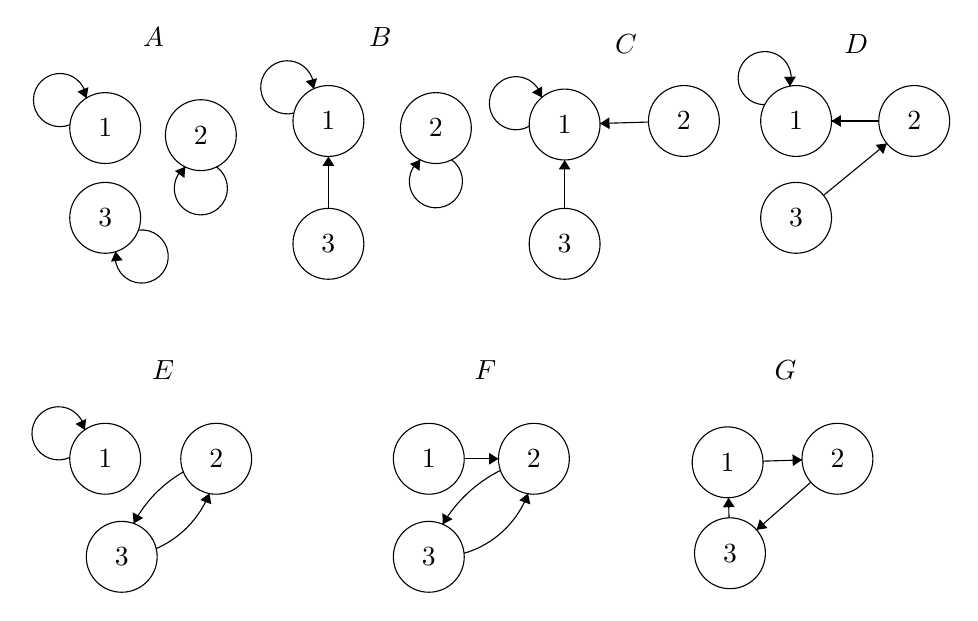
\begin{tikzpicture}[scale=0.15]
    \tikzstyle{every node}+=[inner sep=0pt]
    % \draw [black] (11.4,-11.3) circle (3);
    \draw (11.4,-11.3) node {$A$};
    % \draw [black] (30.6,-11.3) circle (3);
    \draw (30.6,-11.3) node {$B$};
    % \draw [black] (51.4,-11.9) circle (3);
    \draw (51.4,-11.9) node {$C$};
    % \draw [black] (70.9,-11.9) circle (3);
    \draw (70.9,-11.9) node {$D$};
    % \draw [black] (12.2,-39.5) circle (3);
    \draw (12.2,-39.5) node {$E$};
    % \draw [black] (39.5,-39.5) circle (3);
    \draw (39.5,-39.5) node {$F$};
    % \draw [black] (64.9,-39.5) circle (3);
    \draw (64.9,-39.5) node {$G$};
    \draw [black] (7.3,-19) circle (3);
    \draw (7.3,-19) node {$1$};
    \draw [black] (7.3,-26.6) circle (3);
    \draw (7.3,-26.6) node {$3$};
    \draw [black] (15.4,-19.6) circle (3);
    \draw (15.4,-19.6) node {$2$};
    \draw [black] (26.2,-18.4) circle (3);
    \draw (26.2,-18.4) node {$1$};
    \draw [black] (26.2,-28.8) circle (3);
    \draw (26.2,-28.8) node {$3$};
    \draw [black] (35.3,-19) circle (3);
    \draw (35.3,-19) node {$2$};
    \draw [black] (46.2,-18.7) circle (3);
    \draw (46.2,-18.7) node {$1$};
    \draw [black] (46.2,-28.8) circle (3);
    \draw (46.2,-28.8) node {$3$};
    \draw [black] (56.3,-18.4) circle (3);
    \draw (56.3,-18.4) node {$2$};
    \draw [black] (65.8,-18.4) circle (3);
    \draw (65.8,-18.4) node {$1$};
    \draw [black] (65.8,-26.6) circle (3);
    \draw (65.8,-26.6) node {$3$};
    \draw [black] (75.8,-18.4) circle (3);
    \draw (75.8,-18.4) node {$2$};
    \draw [black] (34.7,-47) circle (3);
    \draw (34.7,-47) node {$1$};
    \draw [black] (34.7,-55.3) circle (3);
    \draw (34.7,-55.3) node {$3$};
    \draw [black] (43.6,-47) circle (3);
    \draw (43.6,-47) node {$2$};
    \draw [black] (60,-47.3) circle (3);
    \draw (60,-47.3) node {$1$};
    \draw [black] (60.2,-55) circle (3);
    \draw (60.2,-55) node {$3$};
    \draw [black] (69.3,-47) circle (3);
    \draw (69.3,-47) node {$2$};
    \draw [black] (7.3,-47) circle (3);
    \draw (7.3,-47) node {$1$};
    \draw [black] (8.7,-55.3) circle (3);
    \draw (8.7,-55.3) node {$3$};
    \draw [black] (16.7,-47) circle (3);
    \draw (16.7,-47) node {$2$};
    \draw [black] (4.325,-18.714) arc (292.24052:4.24052:2.25);
    \fill [black] (5.72,-16.47) -- (5.88,-15.54) -- (4.95,-15.91);
    \draw [black] (10.101,-27.64) arc (97.36342:-190.63658:2.25);
    \fill [black] (8.18,-29.46) -- (7.79,-30.31) -- (8.78,-30.19);
    \draw [black] (16.723,-22.28) arc (54:-234:2.25);
    \fill [black] (14.08,-22.28) -- (13.2,-22.63) -- (14.01,-23.22);
    \draw [black] (26.2,-25.8) -- (26.2,-21.4);
    \fill [black] (26.2,-21.4) -- (25.7,-22.2) -- (26.7,-22.2);
    \draw [black] (23.289,-17.727) arc (284.71059:-3.28941:2.25);
    \fill [black] (24.96,-15.68) -- (25.24,-14.78) -- (24.28,-15.03);
    \draw [black] (36.623,-21.68) arc (54:-234:2.25);
    \fill [black] (33.98,-21.68) -- (33.1,-22.03) -- (33.91,-22.62);
    \draw [black] (46.2,-25.8) -- (46.2,-21.7);
    \fill [black] (46.2,-21.7) -- (45.7,-22.5) -- (46.7,-22.5);
    \draw [black] (43.215,-18.838) arc (300.37062:12.37062:2.25);
    \fill [black] (44.28,-16.41) -- (44.3,-15.47) -- (43.44,-15.98);
    \draw [black] (53.3,-18.49) -- (49.2,-18.61);
    \fill [black] (49.2,-18.61) -- (50.01,-19.09) -- (49.98,-18.09);
    \draw [black] (68.12,-24.7) -- (73.48,-20.3);
    \fill [black] (73.48,-20.3) -- (72.54,-20.42) -- (73.18,-21.2);
    \draw [black] (72.8,-18.4) -- (68.8,-18.4);
    \fill [black] (68.8,-18.4) -- (69.6,-18.9) -- (69.6,-17.9);
    \draw [black] (63.149,-17.021) arc (270.25384:-17.74616:2.25);
    \fill [black] (65.28,-15.46) -- (65.78,-14.65) -- (64.78,-14.66);
    \draw [black] (16.12,-49.927) arc (-21.35064:-66.54055:8.469);
    \fill [black] (16.12,-49.93) -- (15.36,-50.49) -- (16.29,-50.85);
    \draw [black] (9.706,-52.484) arc (152.38382:119.72499:10.806);
    \fill [black] (9.71,-52.48) -- (10.52,-52.01) -- (9.63,-51.54);
    \draw [black] (4.314,-46.878) arc (295.38954:7.38954:2.25);
    \fill [black] (5.58,-44.56) -- (5.69,-43.62) -- (4.79,-44.05);
    \draw [black] (43.101,-49.941) arc (-20.09413:-73.90163:8.208);
    \fill [black] (43.1,-49.94) -- (42.36,-50.52) -- (43.3,-50.86);
    \draw [black] (35.876,-52.549) arc (149.54048:116.46376:11.763);
    \fill [black] (35.88,-52.55) -- (36.71,-52.11) -- (35.85,-51.61);
    \draw [black] (37.7,-47) -- (40.6,-47);
    \fill [black] (40.6,-47) -- (39.8,-46.5) -- (39.8,-47.5);
    \draw [black] (67.05,-48.98) -- (62.45,-53.02);
    \fill [black] (62.45,-53.02) -- (63.38,-52.87) -- (62.72,-52.12);
    \draw [black] (60.12,-52) -- (60.08,-50.3);
    \fill [black] (60.08,-50.3) -- (59.6,-51.11) -- (60.6,-51.09);
    \draw [black] (63,-47.2) -- (66.3,-47.1);
    \fill [black] (66.3,-47.1) -- (65.49,-46.62) -- (65.52,-47.62);
    \end{tikzpicture}
    \end{center}

    \item Let $O_1 = \{1\}, O_2 = \{2\}, O_3 = \{3\}, O_4 = \{2, 3\}, O_5 = \{1, 2, 3\}$. Then 
    \begin{itemize}
        \item $\autorbs{A} = \{O_5\}$. This can be defined by the schema $(\forall x)(x = x)$. 

        \item $\autorbs{B} = \{O_1, O_2, O_3\}$. $O_1$ can be defined by $Lxx \land (\exists y)(Lyx \land y \neq x)$, $O_2$ can be defined by $Lxx \land \lnot (\exists y)(Lyx \land y \neq x)$, and $O_3$ can be defined by $\lnot Lxx$. 

        \item $\autorbs{C} = \{O_1, O_4\}$. $O_1$ can be defined by $Lxx$, and $O_4$ can be defined by $\lnot Lxx$. 

        \item $\autorbs{D} = \{O_1, O_2, O_3\}$. $O_1$ can be defined by $Lxx$, $O_2$ can be defined by $(\exists y)(Lyx \land x \neq y)$, and $O_3$ can be defined by $\lnot (\exists y)Lyx$. 

        \item $\autorbs{E} = \{O_1, O_4\}$. $O_1$ can be defined by $Lxx$, and $O_4$ can be defined by $\lnot Lxx$. 

        \item $\autorbs{F} = \{O_1, O_2, O_3\}$. $O_1$ can be defined by $\lnot (\exists y)Lyx$, $O_2$ can be defined by $(\exists yz)(Lyx \land Lxz \land z \neq y)$, and $O_3$ can be defined by $(\exists y)(\forall z)(Lzx \equiv y = z)$. 

        \item $\autorbs{G} = \{O_5\}$. This can be defined by the schema $(\forall x)(x = x)$. 
    \end{itemize}

    \item Yes, it is definable. $P^A$ is the \emph{distance relation}; $\langle i, j, k \rangle \in P^A$ iff the distance between $i, j$ is $k$. No two numbers have a negative distance, so we can define the set of all negative numbers by the schema
    \[
        (\forall yz)(\lnot Pyzx)
    \]

    \item No, it is not definable. The function $h$ defined by $h(i) = -i$ is an automorphism of $B$, but $h[X] \neq X$. 

    \item Yes, $X$ does imply $S$. Here is a derivation
    \[
\begin{array}{lll}
\{1\}   & (1)\ (\exists y)(\forall x)(Lxy \vee Lyx)  & \mathrm{P}\\
\{1, 2\} & (2)\ (\forall x)(Lxy \vee Lyx) & (1)y\ \mathrm{EII}\\
\{1, 2\} & (3)\ (Lxy \vee Lyx) & (2)\ \mathrm{UI}\\
\{1, 2\} & (4)\ (\exists y)(Lxy \vee Lyx) & (3)\ \mathrm{EG}\\
\{1\} & (5)\ (\exists y)(Lxy \vee Lyx) & (4)\{2\}\ \mathrm{EIE}\\
\{1\} & (6)\ (\forall x)(\exists y)(Lxy \vee Lyx) & (5)\ \mathrm{UG}
\end{array}
\]

    \item $X$ does not imply $S$. $X$ states that we have a simple graph of size 5, and $S$ expresses the \emph{three-mutuality} that we considered on day 1 of class. We shows that a ``friendship pentagon'' lacked 3-mutuality; that same pentagon acts as a counterexample here. 

    \item Yes, it is. To show this, we give a satisfying model for $X$. Recall that $\mathbb{Z}$ is the set of integers and $\mathbb{Q}^+$ is the set of positive rational numbers. Let $A$ be defined by
    \begin{itemize}
    \item
    $U^A= \mathbb{Q}^+\times\mathbb{Z}=\{\op{r}{i}\mid r\in\mathbb{Q}^+\mbox{ and}\ i\in \mathbb{Z}\}$ (the cartesian product of $\mathbb{Q}^+$ and $\mathbb{Z}$).
    \item
    $L^A=\{\op{\op{r}{i}}{\op{s}{j}}\mid r<s\}\cup\{\op{\op{r}{i}}{\op{s}{j}}\mid r=s\mbox{ and }i<j\}$.
    \end{itemize}

    Then $A \models X$. 

    \item Yes, it is. We show that $X$ is satisfiable by constructing a structure $B$ with $B\models X$. $B$ is defined by
    \begin{itemize}
    \item
    $U^B= \mathbb{Z}^+$.
    \item
    $F^B=\{2i\mid i\in\mathbb{Z}^+\}$.
    \item
    $L^B = \{\op{2^i\cdot j}{j}\mid i\in\mathbb{Z}^+\mbox{ and } j\not\in F^B\}$.
    \end{itemize}

\end{enumerate}
\end{mdframed}
\newpage

\section{Appendix: A Proof of the Compactness Theorem}
We prove the Compactness Theorem for First-Order Logic (PQT). 

\begin{theorem}(Compactness)
Let $T$ be a set of schemata. If every finite $T_0 \subseteq T$ is satisfiable, $T$ is satisfiable. 
\end{theorem}

\begin{definition}
Let $X$ be a nonempty set. A collection $\mathcal{F}$ of subsets of $X$ has the \emph{finite intersection property} if every (nonempty) finite intersection of sets in $\mathcal{F}$ is nonempty. 
\end{definition}

\begin{definition}
Let $X$ be a nonempty set. A collection $\mathcal{F}$ of subsets of $X$ is a \emph{filter} iff
\begin{enumerate}
    \item $\mathcal{F} \neq \emptyset$
    \item $\emptyset \not \in \mathcal{F}$
    \item $A, B \in \mathcal{F}$ implies $A \cap B \in \mathcal{F}$ ($\mathcal{F}$ is \emph{closed under intersection})
    \item $A \in \mathcal{F}$ and $A \subseteq B \subseteq X$ implies $B \in \mathcal{F}$ ($\mathcal{F}$ is \emph{closed under supersets}). 
\end{enumerate}
\end{definition}


\begin{lemma}
Suppose $\mathcal{F}$ is acollection of subsets of $X$ with the finite intersection property. Let $\mathcal{F}'$ be the collection of nonempty finite intersections of elements of $\mathcal{F}$, and let 
\[
    \mathcal{F}^* := \{Y \subseteq X \mid (\exists Z \in \mathcal{F}')(Z \subseteq Y)\}
\]
Then $\mathcal{F}^*$ is a filter. 
\end{lemma}
\begin{aside}
    Prove that each of the properties of a filter hold for $\mathcal{F}^*$. For example, $(1)$ holds because $\mathcal{F}$ is nonempty, and $(2)$ follows from the finite intersection property. 
\end{aside}

\begin{definition}
An \emph{ultrafilter} $\mathcal{U}$ on a set $X$ is maximal filter (wrt containment), eg if $\mathcal{U} \subseteq \mathcal{U}'$ and $\mathcal{U}'$ is also a filter on $X$, then $\mathcal{U} = \mathcal{U}'$. 
\end{definition}

\end{document}
